\documentclass{article}
\bibliographystyle{livrevrel}

\usepackage{epubtk}
\usepackage{graphicx}
\usepackage{amsmath}
\usepackage{amssymb}
\usepackage{latexsym}
\usepackage{color}

\newcommand{\Msun}{\,M$_{\odot}$}

\begin{document}

\title{Gravitational Wave Detection by Interferometry \\(Ground and Space)}

\author{%
\epubtkAuthorData{Matthew Pitkin}
        {SUPA \\
        School of Physics and Astronomy \\
        University of Glasgow \\
        Glasgow G12 8QQ, U.K.}
        {matthew.pitkin@glasgow.ac.uk}
        {}
\and
\epubtkAuthorData{Stuart Reid}
        {SUPA \\
        School of Physics and Astronomy \\
        University of Glasgow \\
        Glasgow G12 8QQ, U.K.}
        {stuart.reid.2@glasgow.ac.uk}
    {}
\and
\epubtkAuthorData{Sheila Rowan}
        {SUPA \\
        School of Physics and Astronomy \\
        University of Glasgow \\
        Glasgow G12 8QQ, U.K.}
        {sheila.rowan@glasgow.ac.uk}
        {}
\and
\epubtkAuthorData{Jim Hough}
        {SUPA \\
        School of Physics and Astronomy \\
        University of Glasgow \\
        Glasgow G12 8QQ, U.K.}
        {james.hough@glasgow.ac.uk}
        {}
}

\date{}
\maketitle

\epubtkKeywords{gravitational waves, laser interferometry}



%%%%%%%%%%%%%%%%%%%%%%%%%%%%%%%%%%%%%%%%%%%%%%%%%%%%%%%%%%%%%%%%%%%%%%%%%%%%%%%%%%%

\begin{abstract}
  Significant progress has been made in recent years on the development of
  gravitational wave detectors. Sources such as coalescing compact binary
  systems, neutron stars in low-mass X-ray binaries, stellar collapses and
  pulsars are all possible candidates for detection. The most promising design
  of gravitational wave detector uses test masses a long distance apart and
  freely suspended as pendulums on Earth or in drag-free craft in space.  The
  main theme of this review is a discussion of the mechanical and optical
  principles used in the various long baseline systems in operation around the
  world -- LIGO (USA), Virgo (Italy/France), TAMA~300 and LCGT (Japan), and GEO~600
  (Germany/U.K.) -- and in LISA, a proposed space-borne interferometer. A review of recent science runs from the current generation of ground-based
  detectors will be discussed, in addition to highlighting the astrophysical results gained thus far.  Looking to the future, the major
  upgrades to LIGO (Advanced LIGO), Virgo (Advanced Virgo), LCGT and GEO600 (GEO-HF) will be completed over the coming years, which will create the first
  network of detectors with the sensitivity required to detect gravitational waves.  Beyond this, the concept and design of possible future ``third generation''
  gravitational wave detectors, such as the Einstein Telescope (ET), will be discussed.
\end{abstract}



%%%%%%%%%%%%%%%%%%%%%%%%%%%%%%%%%%%%%%%%%%%%%%%%%%%%%%%%%%%%%%%%%%%%%%%%%%%%%%%%
%%%
%%%%%%%%%%%%%%%%%%%%%%%%%%%%%%%%%%%%%%%%%%%%%%%%%%%%%%%%%%%%%%%%%%%%%%%%%%%%%%%%
%%%
%%%%%%%%%%%%%%%%%%%%%%%%%%%%%%%%%%%%%%%%%%%%%%%%%%%%%%%%%%%%%%%%%%%%%%%%%%%%%%%%
%%%

\newpage

\section{Introduction}
\label{section:introduction}

Gravitational waves, one of the more exotic predictions of Einstein's General
Theory of Relativity may, after decades of controversy over their existence, be
detected within the next five years.

Sources such as interacting black holes, coalescing compact binary systems,
stellar collapses and pulsars are all possible candidates for detection;
observing signals from them will significantly boost our understanding of the
Universe. New unexpected sources will almost certainly be found and time will
tell what new information such discoveries will bring. Gravitational waves are
ripples in the curvature of space-time and manifest themselves as fluctuating
tidal forces on masses in the path of the wave. The first gravitational wave
detectors were based on the effect of these forces on the fundamental resonant
mode of aluminium bars at room temperature. Initial instruments were constructed
by Joseph Weber~\cite{Weber1, Weber2} and subsequently developed by others.
Reviews of this early work are given in~\cite{Tyson, Douglass}. Following the
lack of confirmed detection of signals, aluminium bar systems operated at and
below the temperature of liquid helium were developed~\cite{Astone, Prodi,
Amaldi, Heng},
%and work in this area is still underway~\cite{Astone, Prodi, Amaldi, Heng}.
although work in this area is now subsiding, with only two detectors, Auriga~\cite{AURIGA} and Nautilus~\cite{NAUTILUS}, continuing to operate. Effort also continues to be pursued into cryogenic spherical bar detectors,
which are designed to have a wider bandwidth than the cylindrical bars, with the
two proto-types detectors the Dutch MiniGRAIL~\cite{MiniGRAIL, Gottardi:2007}
and Brazilian M\'{a}rio Schenberg \cite{Schenberg, Aguiar:2006}. However the
most promising design of gravitational wave detectors, offering the possibility
of very high sensitivities over a wide range of frequency, uses widely separated
test masses freely suspended as pendulums on Earth or in a drag free craft in
space; laser interferometry provides a means of sensing the motion of the masses
produced as they interact with a gravitational wave.

Ground based detectors of this type, based on the pioneering work of Bob Forward
and colleagues (Hughes Aircraft)~\cite{Forward}, Rai Weiss and colleagues (MIT)
\cite{Weiss}, Ron Drever and colleagues (Glasgow/Caltech) \cite{Drever1,
Drever2} and Heinz Billing and colleagues (MPQ Garching)~\cite{Billing}, will be
used to observe sources whose radiation is emitted at frequencies above a few
Hz, and space borne detectors, as originally envisaged by Peter Bender and Jim
Faller~\cite{BenderFaller1, BenderFaller2} at JILA, will be developed for
implementation at lower frequencies.

Gravitational wave detectors of long baseline have been built in a number of
places around the world; in the USA (LIGO project led by a Caltech/MIT
consortium)~\cite{LIGOS5, LIGOweb}, in Italy (Virgo project, a joint
Italian/French venture)~\cite{Acernese:2007, Virgoweb}, in Germany (GEO~600
project built by a collaboration centred on the University of Glasgow, the
University of Hannover, the Max Planck Institute for Quantum Optics, the Max
Planck Institute for Gravitational Physics (Albert Einstein Institute), Golm and
Cardiff University)~\cite{Willke:2007, GEOweb} and in Japan (TAMA~300
project)~\cite{TAMAStatus, TAMAweb}. A space-borne detector, LISA,~\cite{LISA,
NASAweb, ESAweb} -- proposed by a collaboration of European and US research
groups -- has been adopted by ESA as a future Cosmic Vision Mission and the NASA
Beyond Einstein program. When completed, this detector array should have the
capability of detecting gravitational wave signals from violent astrophysical
events in the Universe, providing unique information on testing aspects of
General Relativity and opening up a new field of astronomy.

It is also be possible to observe the tidal effects of a passing gravitational wave by Doppler tracking of separated objects.  For example, Doppler tracking of spacecraft allows the Earth and an interplanetary spacecraft to be used as test masses, where their relative positions can be monitored by comparing the nearly monochromatic microwave signal sent from a ground station with the coherently returned signal sent from the spacecraft.  By comparing these signals, a Doppler frequency time series $\Delta \nu / \nu_0$, where $\nu_0$ is the central frequency from the ground station, can be generated.  Peculiar characteristics within the Doppler time series, caused by the passing of gravitational waves, can be studied in the approximate frequency band of $10^{-5}$ to $0.1$ Hz.  Several attempts have been made in recent decades to collect such data (Ulysses, Mars Observer, Galileo, Mars Global Surveyor, Cassini) with broadband frequency sensitivities reaching $10^{-16}$. There are currently no plans for dedicated experiments using this technique, however incorporating Doppler tracking into another planetary mission would provide a complimentary precursor mission before dedicated experiments such as LISA are launched.

The technique of Doppler tracking to search for gravitational wave signals can also be performed using pulsar timing experiments.  Millisecond pulsars \cite{Lorimer:2008} are known to be very precise clocks, which allows the effects of a passing gravitational wave to be observed through the modulation in the time of arrival of pulses from the pulsar.  Many noise sources exist and, for this reason, it is necessary to monitor a large array of pulsars over a long observation time.  Further details on the techniques used and upper limits that have been set with pulsar timing experiments can be found from groups such as the European Pulsar Timing Array~\cite{Janssen:2008}, the North American Nanohertz Observatory for Gravitational Waves~\cite{Jenet:2006,Jenet:2009}, and the Parkes Pulsar Timing Array~\cite{Hobbs:2008}.

We recommend a number of excellent books for reference. For a popular account of the development of the gravitational wave field the reader should consult Chapter~10 of `Black Holes and Time Warps' by Kip S.\ Thorne~\cite{Thorne}, or the more recent books, `Einstein's Unfinished Symphony', by Marcia Bartusiak~\cite{Bartusiak:2003} and `Gravity from the Ground Up', by Bernard Schutz~\cite{Schutz:2003}. A comprehensive review of developments toward laser interferometer detectors is found in `Fundamentals of Interferometric Gravitational Wave Detectors' by Peter Saulson~\cite{Saulsonbook}, and discussions relevant to the technology of both bar and interferometric detectors are found in `The Detection of Gravitational Waves' edited by David Blair~\cite{Blair}.

In addition to the wealth of articles that can be found on the home site of this journal, there are also various informative websites that can be easily found, including the homepages of the various international collaborative projects searching for gravitational waves, such as the LIGO Scientific Collaboration~\cite{LSCweb}.

\newpage

%%%%%%%%%%%%%%%%%%%%%%%%%%%%%%%%%%%%%%%%%%%%%%%%%%%%%%%%%%%%%%%%%%%%%%%%%%%%%%%%
%%%%%%%%%%%%%%%%%%%%%%%%%%%%%%%%%%%%%%%%%%%%%%%%%%%%%%%%%%%%%%%%%%%%%%%%%%%%%%%%

\section{Gravitational Waves}
\label{section:gravwaves}

Some early relativists were sceptical about the existence of gravitational
waves; however, the 1993 Nobel Prize in Physics was awarded to Hulse and Taylor
for their experimental observations and subsequent interpretations of the
evolution of the orbit of the binary pulsar PSR 1913+16~\cite{Hulse, Taylor},
the decay of the binary orbit being consistent with angular momentum and energy
being carried away from this system by gravitational waves~\cite{Will}.

Gravitational waves are produced when matter is accelerated in an asymmetrical
way; but due to the nature of the gravitational interaction, detectable levels
of radiation are produced only when very large masses are accelerated in very
strong gravitational fields. Such a situation cannot be found on Earth but is
found in a variety of astrophysical systems. Gravitational wave signals are
expected over a wide range of frequencies; from $\simeq 10^{-17}$~Hz in the case
of ripples in the cosmological background to $\simeq 10^3$~Hz from the formation
of neutron stars in supernova explosions. The most predictable sources are
binary star systems. However there are many sources of much greater
astrophysical interest associated with black hole interactions and coalescences,
neutron star coalescences, neutron stars in low-mass X-ray binaries such as
Sco-X1, stellar collapses to neutron stars and black holes (supernova
explosions), pulsars, and the physics of the early Universe. For a full
discussion of sources refer to the material contained in
references~\cite{Sathyaprakash:2009,LISAsymposium, sources, Amaldiproc}.

Why is there currently such interest worldwide in the detection of gravitational
waves? Partly because observation of the velocity and polarisation states of the
signals will allow a direct experimental check of the wave predictions of
General Relativity; but more importantly because the detection of the signals
should provide observers with new and unique information about astrophysical
processes. It is interesting to note that the gravitational wave signal from a
coalescing compact binary star system has a relatively simple form and the
distance to the source can be obtained from a combination of its signal strength
and its evolution in time. If the redshift at that distance is found, Hubble's
Constant -- the value for which has been a source of lively debate for many
years -- may then be determined with, potentially, a high degree of
accuracy~\cite{Schutz,Holtz:2005}.

Only now technology has reached a stage where the building of detectors of the
sensitivity required to observe such interesting sources has been realised.

%%%%%%%%%%%%%%%%%%%%%%%%%%%%%%%%%%%%%%%%%%%%%%%%%%%%%%%%%%%%%%%%%%%%%%%%%%%%%%%%
%%%%%%%%%%%%%%%%%%%%%%%%%%%%%%%%%%%%%%%%%%%%%%%%%%%%%%%%%%%%%%%%%%%%%%%%%%%%%%%%

\newpage

\section{Detection of Gravitational Waves}
\label{section:Detection}

Gravitational waves are most simply thought of as ripples in the curvature of
space-time, their effect being to change the separation of adjacent masses on
earth or in space; this tidal effect is the basis of all present detectors.
Gravitational wave strengths are characterised by the gravitational wave
amplitude h, given by
%
\begin{equation}
  h = \frac{2 \Delta L} L,
  \label{equation:h}
\end{equation}
%
where $\Delta L$ is the change in separation of two masses a distance $L$ apart;
for the strongest allowed component of gravitational radiation the value of $h$
is proportional to the third time derivative of the quadrupole moment of the
source of the radiation and inversely proportional to the distance to the
source. The radiation field itself is quadrupole in nature and this shows up in
the pattern of the interaction of the waves with matter.

The problem for the experimental physicist is that the predicted magnitudes of
the amplitudes or strains in space in the vicinity of the earth caused by
gravitational waves even from the most violent astrophysical events are
extremely small, of the order of $10^{-21}$ or lower~\cite{Sathyaprakash:2009,LISAsymposium}.
Indeed current theoretical models on the event rate and strength of such events
suggest that in order to detect a few events per year -- from coalescing neutron
star binary systems for example -- an amplitude sensitivity close to $10^{-22}$
over timescales as short as a millisecond is required. If the Fourier transform
of a likely signal is considered it is found that the energy of the signal is
distributed over a frequency range or bandwidth which is approximately equal to
1/timescale.  For timescales of a millisecond the bandwidth is approximately
1000~Hz, and in this case the spectral density of the amplitude sensitivity is
obtained by dividing $10^{-22}$ by the square root of 1000. Thus detector noise
levels must have an amplitude spectral density lower than $\simeq 10^{-23}(\rm
Hz)^{-1/2}$ over the frequency range of the signal. Signal strengths at the
earth, integrated over appropriate time intervals, for a number of sources are
shown in Fig.~\ref{figure:sourcestrengths}.

\epubtkImage{}{%
\begin{figure}[hptb]
  \centerline{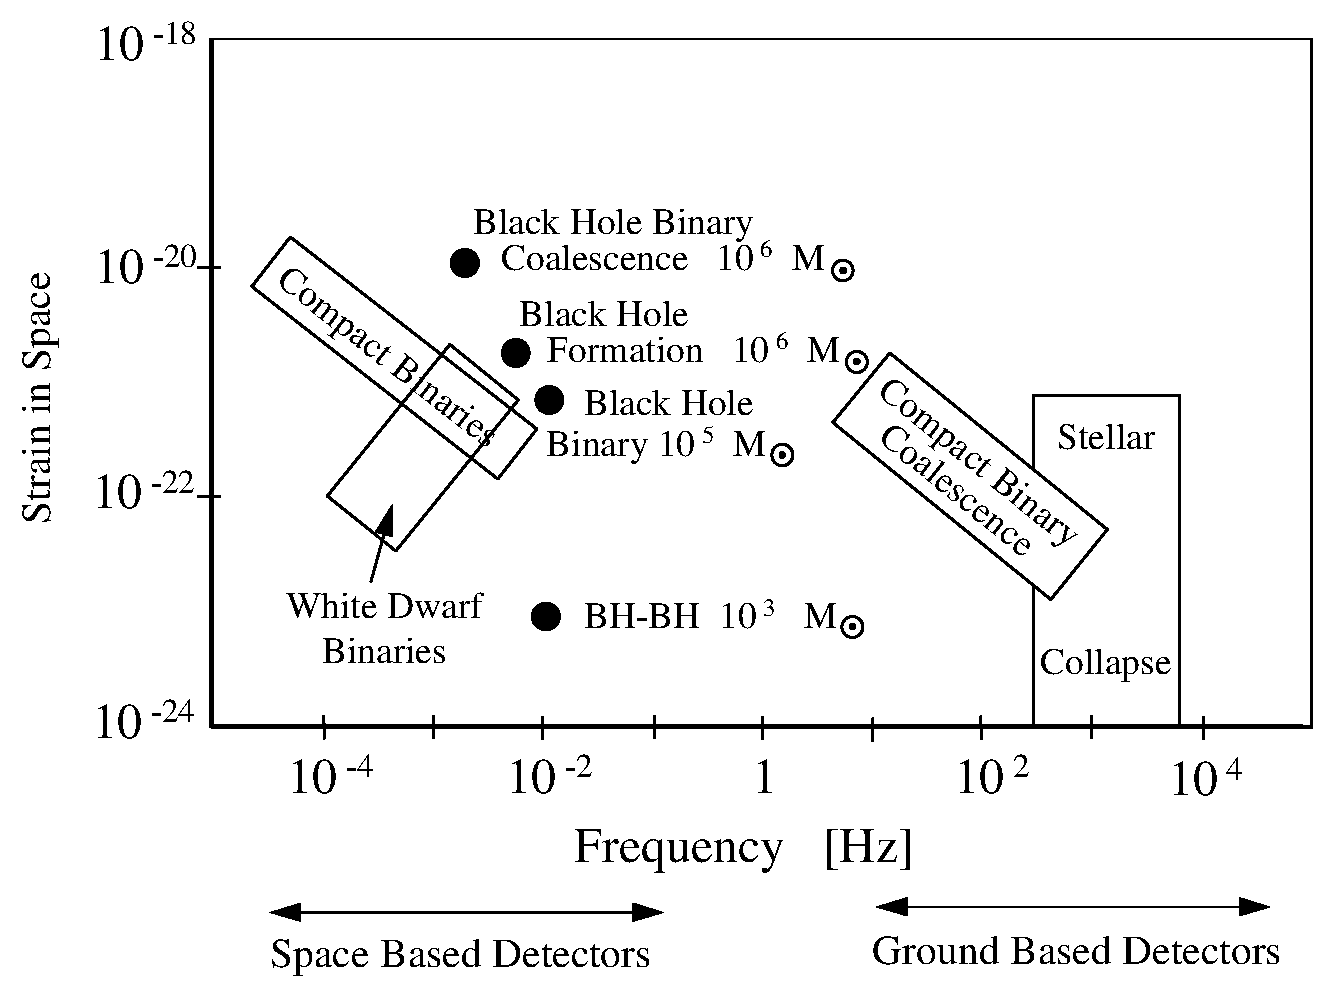
\includegraphics[scale=0.5]{fig1.eps}}
  \caption{\it Some possible sources for ground based and space-borne
    detectors.}
  \label{figure:sourcestrengths}
\end{figure}}

The weakness of the signal means that limiting noise sources like the thermal
motion of molecules in the critical components of the detector (thermal noise), seismic or other mechanical
disturbances, and noise associated with the detector readout, whether electronic
or optical, must be reduced to an extremely low level. For signals above
$\simeq$~10~Hz ground based experiments are possible, but for lower frequencies
where local fluctuating gravitational gradients and seismic noise on earth
become a problem, it is best to consider developing detectors for operation in
space~\cite{LISA}.

%%%%%%%%%%%%%%%%%%%%%%%%%%%%%%%%%%%%%%%%%%%%%%%%%%%%%%%%%%%%%%%%%%%%%%%%%%%%%%%%
%%%%%%%%%%%%%%%%%%%%%%%%%%%%%%%%%%%%%%%%%%%%%%%%%%%%%%%%%%%%%%%%%%%%%%%%%%%%%%%%

\subsection{Initial Detectors and their Development}
\label{subsection:initdet}

The earliest experiments in the field were ground based and were carried out by
Joseph Weber of the University of Maryland in the 1960s. With colleagues
he began by looking for evidence of excitation of the normal modes of the earth
by very low frequency gravitational waves~\cite{Forward2}. Weber then moved on
to look for tidal strains in aluminium bars which were at room temperature and
were well isolated from ground vibrations and acoustic noise in the
laboratory~\cite{Weber1, Weber2}. The bars were resonant at $\simeq$~1600~Hz, a
frequency where the energy spectrum of the signals from collapsing stars was
predicted to peak. Despite the fact that Weber observed coincident excitations
of his detectors placed up to 1000~km apart, at a rate of approximately one
event per day, his results were not substantiated by similar experiments carried
out in several other laboratories in the U.S.A., Germany, Britain and Russia. It
seems unlikely that Weber was observing gravitational wave signals because,
although his detectors were very sensitive, being able to detect strains of the
order of $10^{-16}$ over millisecond timescales~\cite{Weber1}, their sensitivity was far away
from what was predicted to be required theoretically. Development of Weber bar
type detectors continued with significant emphasis on cooling to reduce the noise
levels, although work in this area is now subsiding with efforts continuing on Auriga~\cite{AURIGA}, Nautilus~\cite{NAUTILUS}, MiniGRAIL~\cite{MiniGRAIL, Gottardi:2007}
and M\'{a}rio Schenberg \cite{Schenberg, Aguiar:2006}.  In around 2003, the sensitivity of km-scale interferometric gravitational wave detectors began to surpass the peak sensitivity of these cryogenic bar detectors ($\simeq 10^{-21}$) and, for example, the LIGO detectors reached their design sensitivities at almost all frequencies by 2005 (peak sensitivity $\simeq 2\times10^{-23}$ at $\simeq200$~Hz)~\cite{Whitcomb:2008}.  In addition to gaining better strain sensitivities, interferometric detectors have a marked advantage over resonant bars by being sensitive to a broader range of frequencies, whereas resonant bar are inherently sensitive only to signals that have significant spectral energy in a narrow band around their resonant frequency. The concept and design of gravitational wave detector based on a laser interferometer will be introduced in the following section.


%%%%%%%%%%%%%%%%%%%%%%%%%%%%%%%%%%%%%%%%%%%%%%%%%%%%%%%%%%%%%%%%%%%%%%%%%%%%
%%%%%%%%%%%%%%%%%%%%%%%%%%%%%%%%%%%%%%%%%%%%%%%%%%%%%%%%%%%%%%%%%%%%%%%%%%%%


\subsection{Long Baseline Detectors on Earth}
\label{subsection:earth}

An interferometric design of gravitational wave detector offers the
possibility of very high sensitivities over a wide range of
frequency. It uses test masses which are widely separated and freely
suspended as pendulums to isolate against seismic noise and reduce the
effects of thermal noise; laser interferometry provides a means of
sensing the motion of these masses produced as they interact with a
gravitational wave (Fig.~\ref{figure:schematicdetector}).

\epubtkImage{}{%
\begin{figure}[hptb]
  \centerline{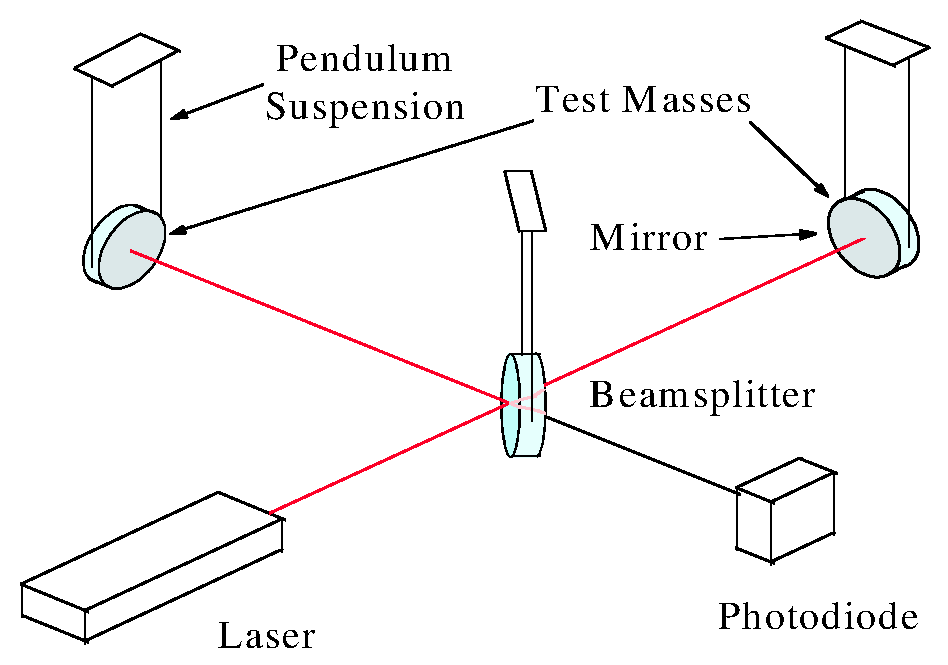
\includegraphics[scale=0.4]{fig2}}
  \caption{\it Schematic of gravitational wave detector using laser
    interferometry.}
  \label{figure:schematicdetector}
\end{figure}}

This technique is based on the Michelson interferometer and is
particularly suited to the detection of gravitational waves as they
have a quadrupole nature. Waves propagating perpendicular to the plane
of the interferometer will result in one arm of the interferometer
being increased in length while the other arm is decreased and vice
versa. The induced change in the length of the interferometer arms results in
a small change in the intensity of the light observed at the
interferometer output.

As will be explained in detail in the next section, the sensitivity of
an interferometric gravitational wave detector is limited by noise
from various sources. Taking this frequency dependent noise floor into
account, a design goal can be estimated for a particular detector design.
For example, the design sensitivity for initial LIGO is show in Fig.~\ref{figure:LIGOsens}
plotted alongside the achieved sensitivities of the three individual interferometers
during the fifth science run. Such strain sensitivities are expected to allow a reasonable
probability for detecting gravitational wave sources. However in order to guarantee the observation
of a full range of sources and to initiate gravitational wave
astronomy, a sensitivity or noise performance approximately ten times
better in the mid-frequency range and several orders of magnitude
better at 10~Hz, is desired. Initial detectors will therefore be upgraded to an Advanced
configuration, such as Advanced LIGO which will be ready for operation around as soon as 2015.

\epubtkImage{}{%
\begin{figure}[hptb]
  \centerline{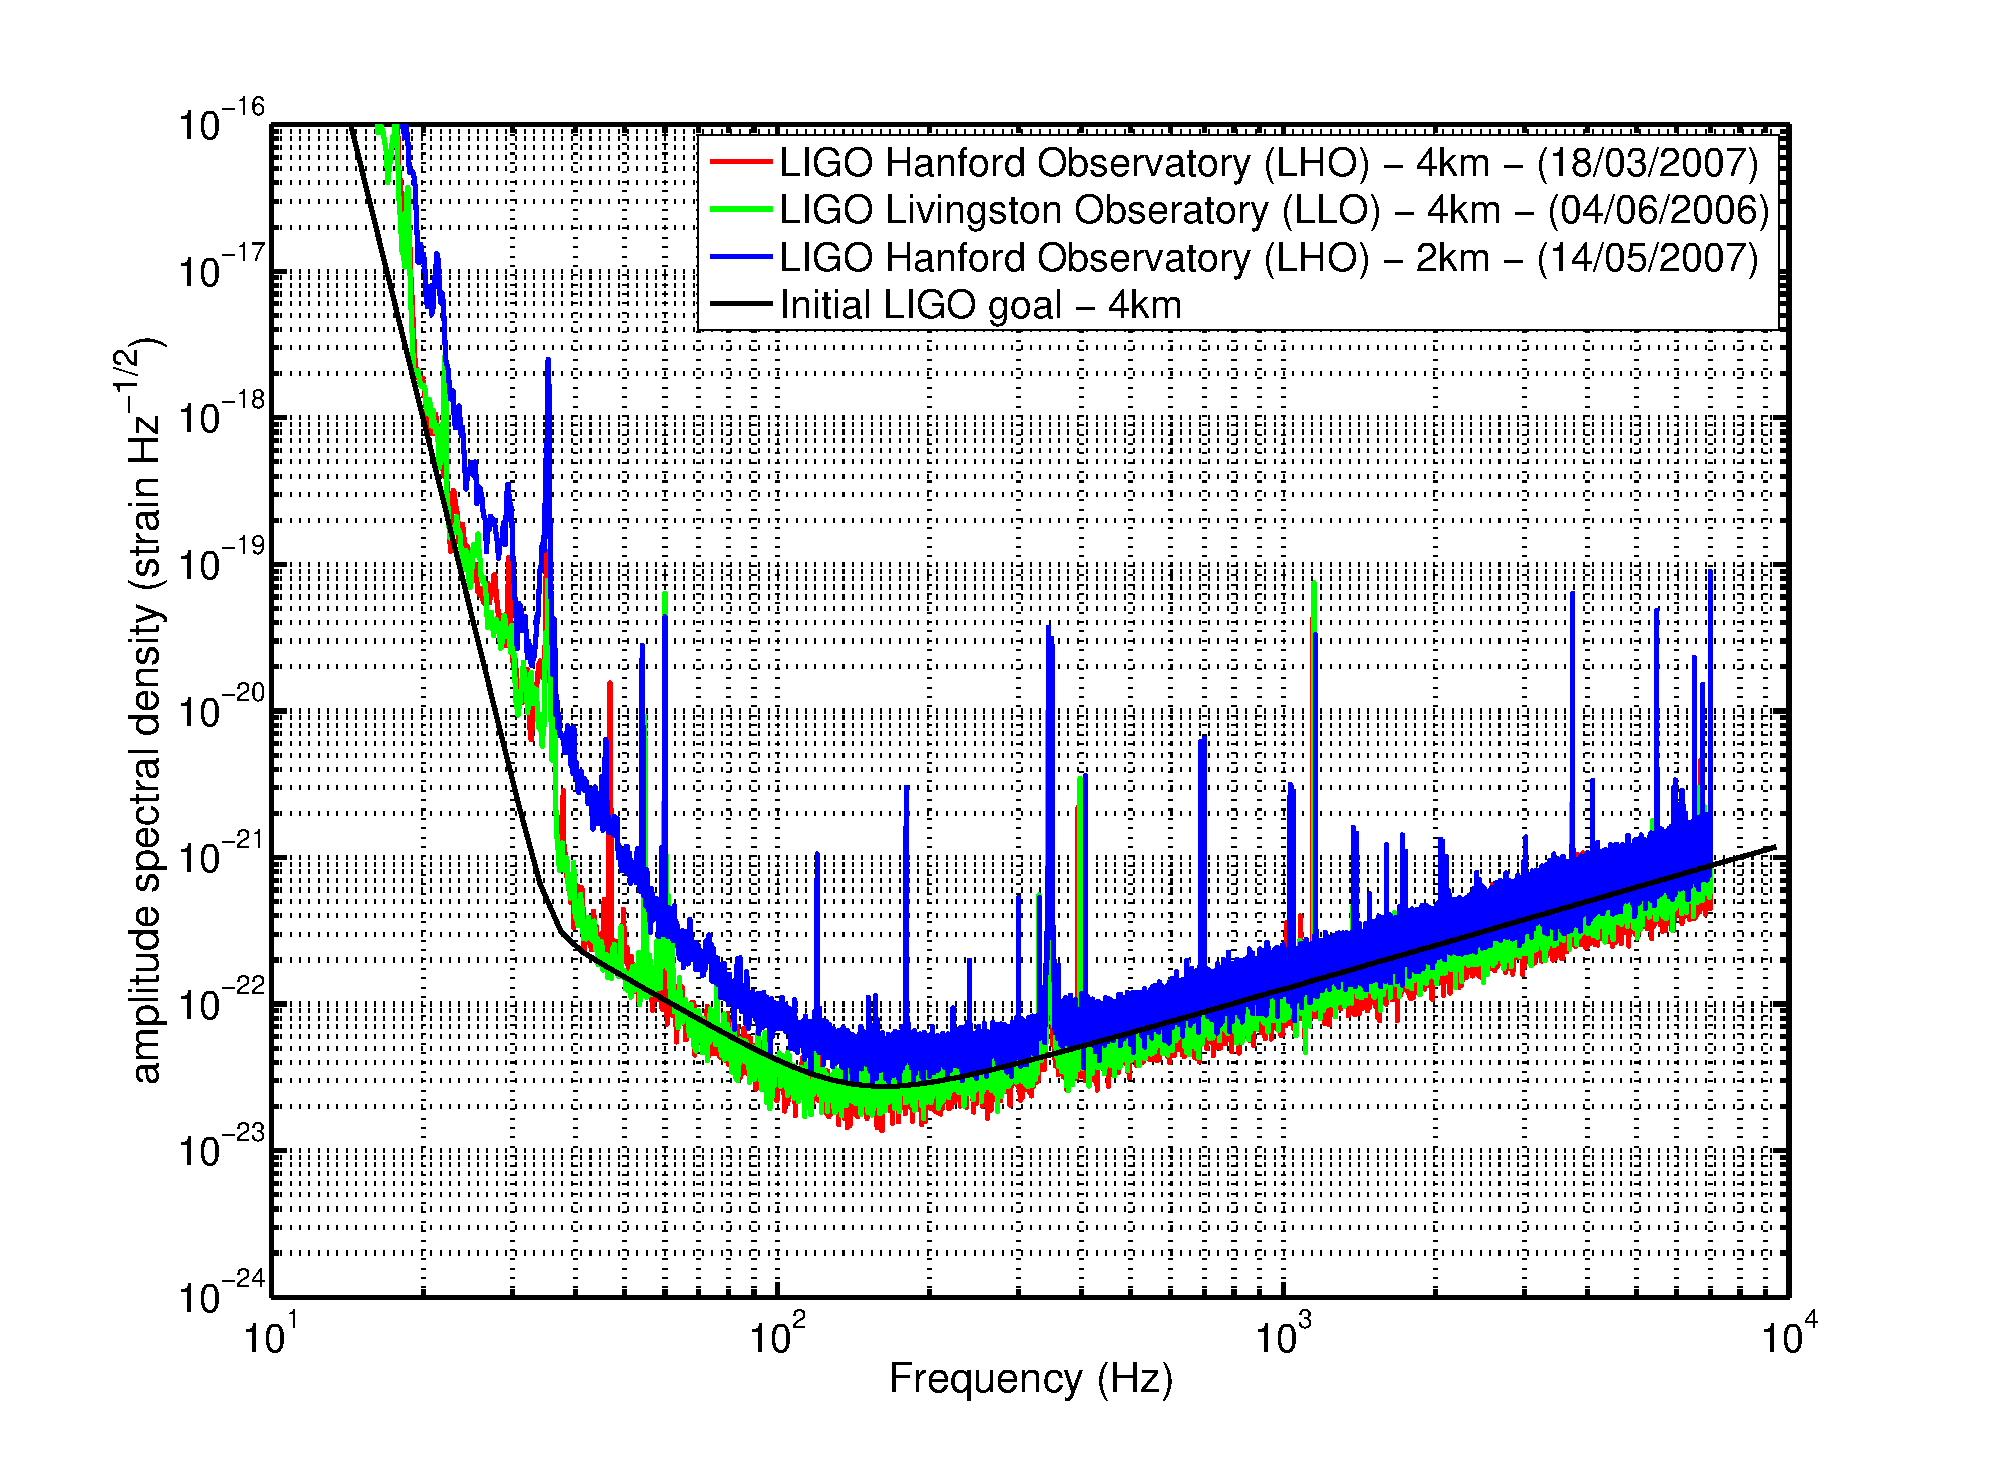
\includegraphics[width=340pt]{LIGOsens}}
  \caption{\it Measured sensitivity of the initial LIGO interferometers.}
  \label{figure:LIGOsens}
\end{figure}}

For the initial interferometric detectors, a noise floor in
strain close to $2 \times 10^{-23}{(\rm Hz)}^{-1/2}$ was achieved.
Detecting a strain in space at this level implies measuring a residual motion of each of the test
masses of about $3 \times 10^{-20} {\rm \ m}(\rm Hz)^{-1/2}$ over part
of the operating range of the detector, which may be from
$\simeq$~10~Hz to a few kHz. Advanced detectors will further push this target down further by
another factor of 10-15. This sets an formidable goal for the
optical detection system at the output of the interferometer.

%%%%%%%%%%%%%%%%%%%%%%%%%%%%%%%%%%%%%%%%%%%%%%%%%%%%%%%%%%%%%%%%%%%%%%%%%%%%%%
%%%%%%%%%%%%%%%%%%%%%%%%%%%%%%%%%%%%%%%%%%%%%%%%%%%%%%%%%%%%%%%%%%%%%%%%%%%%%%
%%%%%%%%%%%%%%%%%%%%%%%%%%%%%%%%%%%%%%%%%%%%%%%%%%%%%%%%%%%%%%%%%%%%%%%%%%%%%%

\newpage

\section{Main Noise Sources}
\label{section:noise}

In this section we discuss the main noise sources which limit the
sensitivity of interferometric gravitational wave
detectors. Fundamentally it should be possible to build systems using
laser interferometry to monitor strains in space which are limited
only by the Heisenberg Uncertainty Principle; however there are other
practical issues which must be taken into account. Fluctuating
gravitational gradients pose one limitation to the interferometer
sensitivity achievable at low frequencies, and it is the level of
noise from this source which dictates that experiments to look for
sub-Hz gravitational wave signals have to be carried out in
space~\cite{Spero, Saulson1, Beccaria, Hughes}. In general, for ground
based detectors the most important limitations to sensitivity result
from the effects of seismic and other ground-borne mechanical noise,
thermal noise associated with the test masses and their suspensions,
and quantum noise, which appears at high frequency as shot noise in the photocurrent from the photodiode which detects
the interference pattern and can appear at low frequency as radiation pressure noise due to momentum transfer to the test masses from the photons when using high laser powers. The significance of each of these sources will be briefly reviewed.

%%%%%%%%%%%%%%%%%%%%%%%%%%%%%%%%%%%%%%%%%%%%%%%%%%%%%%%%%%%%%%%%%%%%%%%%%%%%%
%%%%%%%%%%%%%%%%%%%%%%%%%%%%%%%%%%%%%%%%%%%%%%%%%%%%%%%%%%%%%%%%%%%%%%%%%%%%%

\subsection{Seismic Noise}
\label{subsection:seismic}

Seismic noise at a reasonably quiet site on the earth follows a
spectrum in all three dimensions close to $10^{-7}f^{-2} {\rm \ m}(\rm
Hz)^{-1/2}$ (where here and elsewhere we measure $f$ in Hz) and thus
if the disturbance to each test mass must be less than $3 \times
10^{-20} {\rm \ m}(\rm Hz)^{-1/2}$ at, for example, 30~Hz then the
reduction of seismic noise required at that frequency in the
horizontal direction is greater than $10^{9}$. Since there is liable
to be some coupling of vertical noise through to the horizontal axis,
along which the gravitational wave induced strains are to be sensed, a
significant level of isolation has to be provided in the vertical
direction also. Isolation can be provided in a relatively simple way
by making use of the fact that, for a simple pendulum system, the
transfer function to the pendulum mass of the horizontal motion of the
suspension point falls off as $1/({\rm frequency})^2$ above the
pendulum resonance. In a similar way isolation can be achieved in the
vertical direction by suspending a mass on a spring. In the case of
the Virgo detector system the design allows operation to below 10~Hz
and here a seven stage horizontal pendulum arrangement is adopted with
six of the upper stages being suspended with cantilever springs to
provide vertical isolation~\cite{Braccini}, with similar systems
developed in Australia~\cite{Ju1} and at Caltech~\cite{DeSalvo}. For
the GEO~600 detector, where operation down to 50~Hz was planned, a
triple pendulum system is used with the first two stages being hung
from cantilever springs to provide the vertical isolation necessary to
achieve the desired performance. This arrangement is then hung from a
plate mounted on passive `rubber' isolation mounts and on an active
(electro-mechanical) anti-vibration system~\cite{Plissi1},~\cite{Torrie}. The upgraded seismic isolation for Advanced LIGO will also adopted a variety of active and passive isolation stages. The total isolation will be provided by one external stage (hydraulics), two stages of in-vacuum active isolation, and being completed by the test mass suspensions~\cite{Abbott:2002,Harry:2010}. For clarity, the two stages of in-vacuum isolation is shown in Fig.~\ref{figure:LIGOseismic} whereas the test mass suspensions are shown separately in Fig.~\ref{figure:LIGOquad}.

\epubtkImage{}{%
\begin{figure}[hptb]
  \centerline{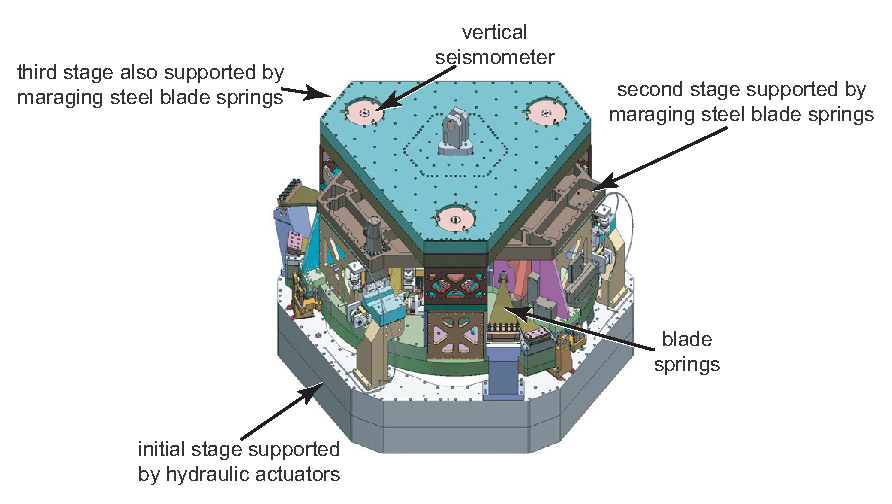
\includegraphics[width=340pt]{fig3}}
  \caption{\it Internal stages of the large chamber seismic isolation system for Advanced LIGO (image is inverted for clarity).}
  \label{figure:LIGOseismic}
\end{figure}}

\epubtkImage{}{%
\begin{figure}[hptb]
  \centerline{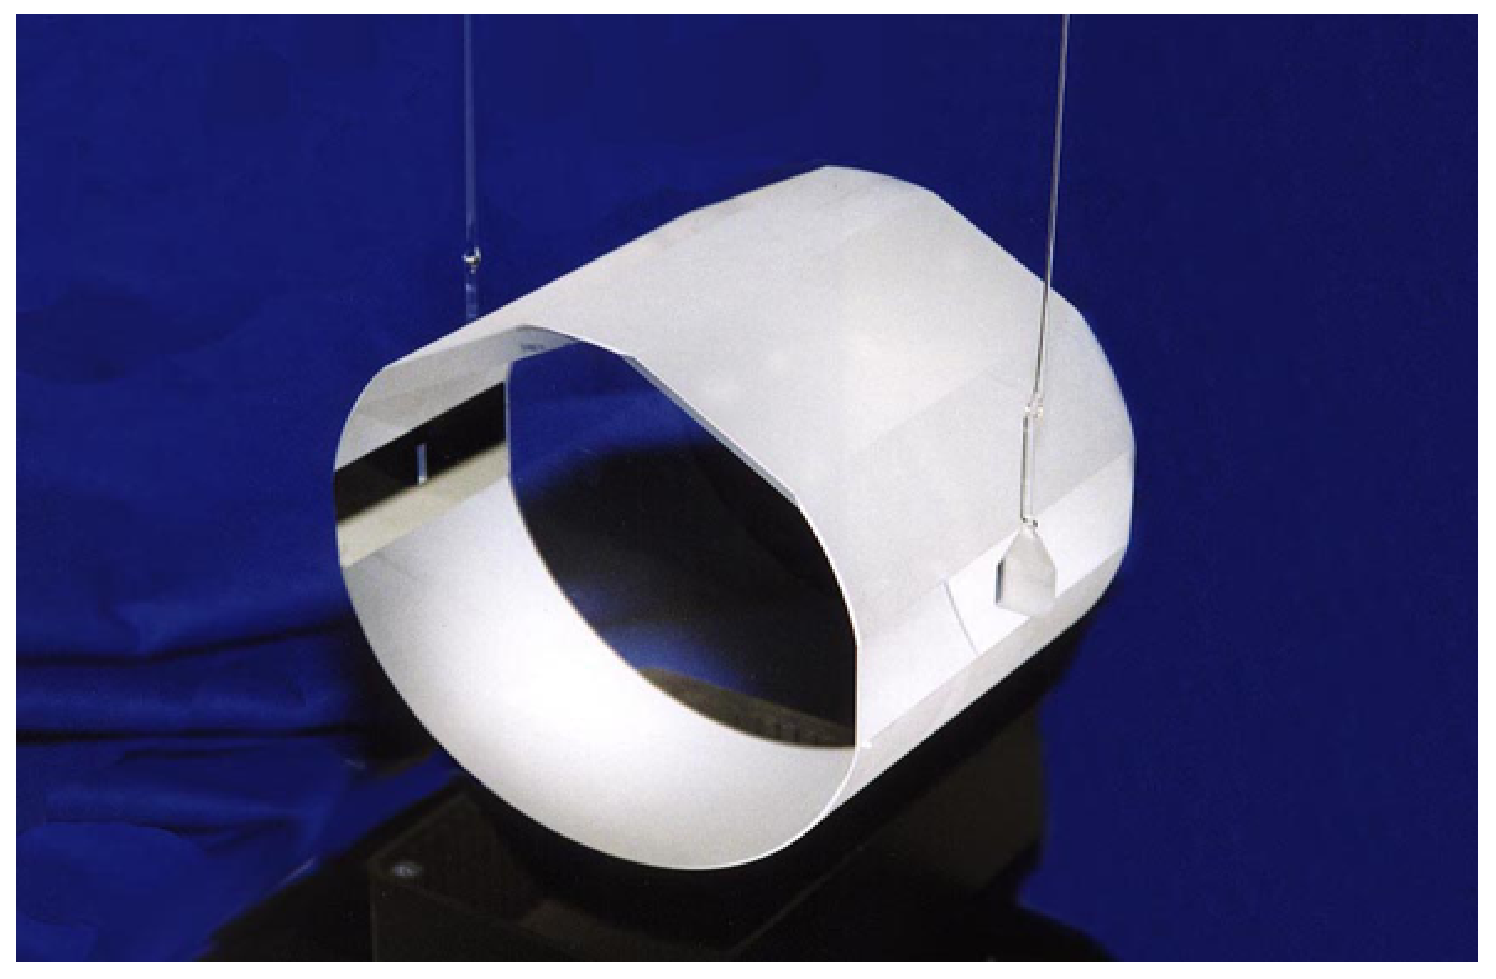
\includegraphics[width=250pt]{fig4}}
  \caption{\it CAD drawing of quad suspension system for Advanced LIGO, showing the mirror test mass at the bottom and where the uppermost section is attached to the third stage platform of the large chamber seismic isolation system shown in Fig.~\ref{figure:LIGOseismic}.}
  \label{figure:LIGOquad}
\end{figure}}

In order to cut down motions at the pendulum frequencies, active
damping of the pendulum modes has to be incorporated, and to reduce
excess motions at low frequencies around the micro-seismic peak, low
frequency isolators have to be incorporated. These low frequency
isolators can take different forms -- tall inverted pendulums in the
horizontal direction and cantilever springs whose stiffness is reduced
by means of attractive forces between magnets for the vertical
direction in the case of the Virgo system~\cite{Losurdo},
Scott-Russell mechanical linkages in the horizontal and torsion bar
arrangements in the vertical for an Australian
design~\cite{Winterflood}, and a seismometer/actuator (active) system as shown here for Advanced LIGO~\cite{Abbott:2002} and also used in
GEO~600~\cite{Plissi2}.

%%%%%%%%%%%%%%%%%%%%%%%%%%%%%%%%%%%%%%%%%%%%%%%%%%%%%%%%%%%%%%%%%%%%%%%%%%%%%%
%%%%%%%%%%%%%%%%%%%%%%%%%%%%%%%%%%%%%%%%%%%%%%%%%%%%%%%%%%%%%%%%%%%%%%%%%%%%%%

\subsection{Gravity Gradient (Newtonian) Noise}
\label{subsection:gravitygradient}

Summary of gravity gradient noise and possible schemes for avoiding (subtraction/underground...)

%%%%%%%%%%%%%%%%%%%%%%%%%%%%%%%%%%%%%%%%%%%%%%%%%%%%%%%%%%%%%%%%%%%%%%%%%%%%%%
%%%%%%%%%%%%%%%%%%%%%%%%%%%%%%%%%%%%%%%%%%%%%%%%%%%%%%%%%%%%%%%%%%%%%%%%%%%%%%

\subsection{Thermal Noise}
\label{subsection:thermal}

Thermal noise associated with the mirror masses and the last stage of
their suspensions is the most significant noise source at
the low frequency end of the operating range of initial long baseline
gravitational wave detectors~\cite{Saulson2}. Advanced detector configurations
are also expected to be limited by thermal noise at their most sensitive frequency
band~\cite{Levin,Nakagawa:2002,Harry:2002,Crooks:2002}. Above the operating range
there are the internal resonances of the test masses. The
thermal noise in the operating range comes from the {\em tails} of
these resonant modes. For any simple harmonic oscillator such as a
mass hung on a spring or hung as a pendulum the spectral density of
thermal motion of the mass can be expressed as~\cite{Saulson2}
%
\begin{equation}
  x^{2}(\omega) = \frac{4 k_{\rm B} T \omega_{0}^{2}
  \phi(\omega)}{\omega m [{(\omega_{0}^{2} - \omega^{2})^2 +
  \omega_{0}^{4} \phi^{2}(\omega)}]},
  \label{equation:thnoise}
\end{equation}
%
where $k_{\rm B}$ is Boltmann's constant, $T$ is the temperature, $m$
is the mass and  $\phi(\omega)$ is the loss angle or loss factor of the
oscillator of angular resonant frequency $\omega_0$.
This loss factor is the phase lag angle between the displacement of the
mass and any force applied to the mass at a frequency well below $\omega_0$.
In the case of a mass on a spring the loss factor is a measure of the
mechanical loss associated with the material of the spring. For a
pendulum, most of the energy is stored in the lossless gravitational
field. Thus the loss factor is lower than that of the material which
is used for the wires or fibres used to suspend the pendulum. Indeed
following Saulson~\cite{Saulson2} it can be shown that for a pendulum
of mass $m$, suspended on four wires or fibres of length $l$, the loss
factor of the pendulum is related to the loss factor of the material
by
%
\begin{equation}
  \phi_{\rm pend}(\omega) = \phi_{\rm mat}(\omega)\frac{4
  \sqrt{TEI}}{mgl},
  \label{equation:pend}
\end{equation}
%
where $I$ is the moment of the cross section of  each wire, and $T$ is
the tension in each wire whose material has a Young's modulus $E$. In
general for most materials it appears that the intrinsic loss factor
is essentially independent of frequency over the range of interest for
gravitational wave detectors (although care has to be taken with some
materials in that a form of damping known as thermo-elastic damping
can become important for wires of small cross-section~\cite{Nowick}
and for some bulk crystalline materials~\cite{Bragthermo}). In order
to estimate the internal thermal noise of a test mass, each resonant
mode of the mass can be regarded as a harmonic oscillator. When the
detector operating range is well below the resonances of the masses,
following Saulson~\cite{Saulson2}, the effective spectral density of
thermal displacement of the front face of each mass can be expressed as:
%
\begin{equation}
  x^{2}(\omega) = \frac{\beta 4 k_{b} T \phi_{\rm mat}(\omega)}{m
  \omega \omega_{0}^{2}}.
  \label{equation:spectraldensity}
\end{equation}
%
In this formula $m$ is the mass of the test mass, $\omega $ is an
angular frequency in the operating range of the detector, $\omega_{0}$
is the resonant angular frequency of the fundamental mode,
$\phi_{\rm mat}(\omega)$ is the intrinsic material loss, and $\beta$
is a correction factor to include the effect of summation of the
motion over the higher order modes of the test mass (taking into
account the effect of a finite optical beam size and correction for
the effective masses of the modes). Typically, as calculated by
Gillespie and Raab~\cite{Gillespie}, $\beta$ is a number less than
10. A different and more general treatment of internal thermal noise
using evaluation of the relevant mechanical impedance has been carried
out by Bondu et al.~\cite{Bondu}. This was based on work of Yuri
Levin~\cite{Levin} and gives good agreement with the results of
Gillespie and Raab.

In order to keep thermal noise as low as possible the mechanical
loss factors of the masses and pendulum resonances should be as
low as possible. Further the test masses must have a shape such that
the frequencies of the internal resonances are kept as high as
possible, must be large enough to accommodate the laser beam spot
without excess diffraction losses, and must be massive enough to keep
the fluctuations due to radiation pressure at an acceptable level. Test
masses range in mass from 6~kg for GEO~600 to 30~kg for the first
proposed upgrade to LIGO. To approach the best levels of sensitivity
discussed earlier the loss factors of the test masses must be $\simeq
3 \times 10^{-8}$ or lower, and the loss factor of the pendulum
resonances should be smaller than $10^{-10}$. Discussions relevant to
this are given in~\cite{Rowan1, RowanTAMA}. Obtaining these values
puts significant constraints on the choice of material for the test
masses and their suspending fibres. One viable solution which should
allow detector sensitivities to approach the level desired for
upgraded detectors is to use fused silica masses hung by fused silica
fibres~\cite{Braginsky1, Rowan2}, as the intrinsic loss factors in
samples of synthetic fused silica have been measured at around $3
\times 10^{-8}$~\cite{Lunin, Startin}. Still, the use of other
materials such as sapphire is being seriously considered for future
detectors as mentioned in
Section~\ref{section:construction}~\cite{Braginsky2, Ju2, Rowan1}. The
technique of hydroxy-catalysis bonding provides a method of jointing
oxide materials in a suitably low loss way to allow `monolithic'
suspension systems to be constructed~\cite{Rowan3}. A picture of such
a prototype fused silica mass suspended by two fused silica fibres,
which has been constructed in Glasgow and is being tested at the
University of Perugia, is shown in Fig.~\ref{figure:silicamass}.

\epubtkImage{}{%
\begin{figure}[hptb]
  \centerline{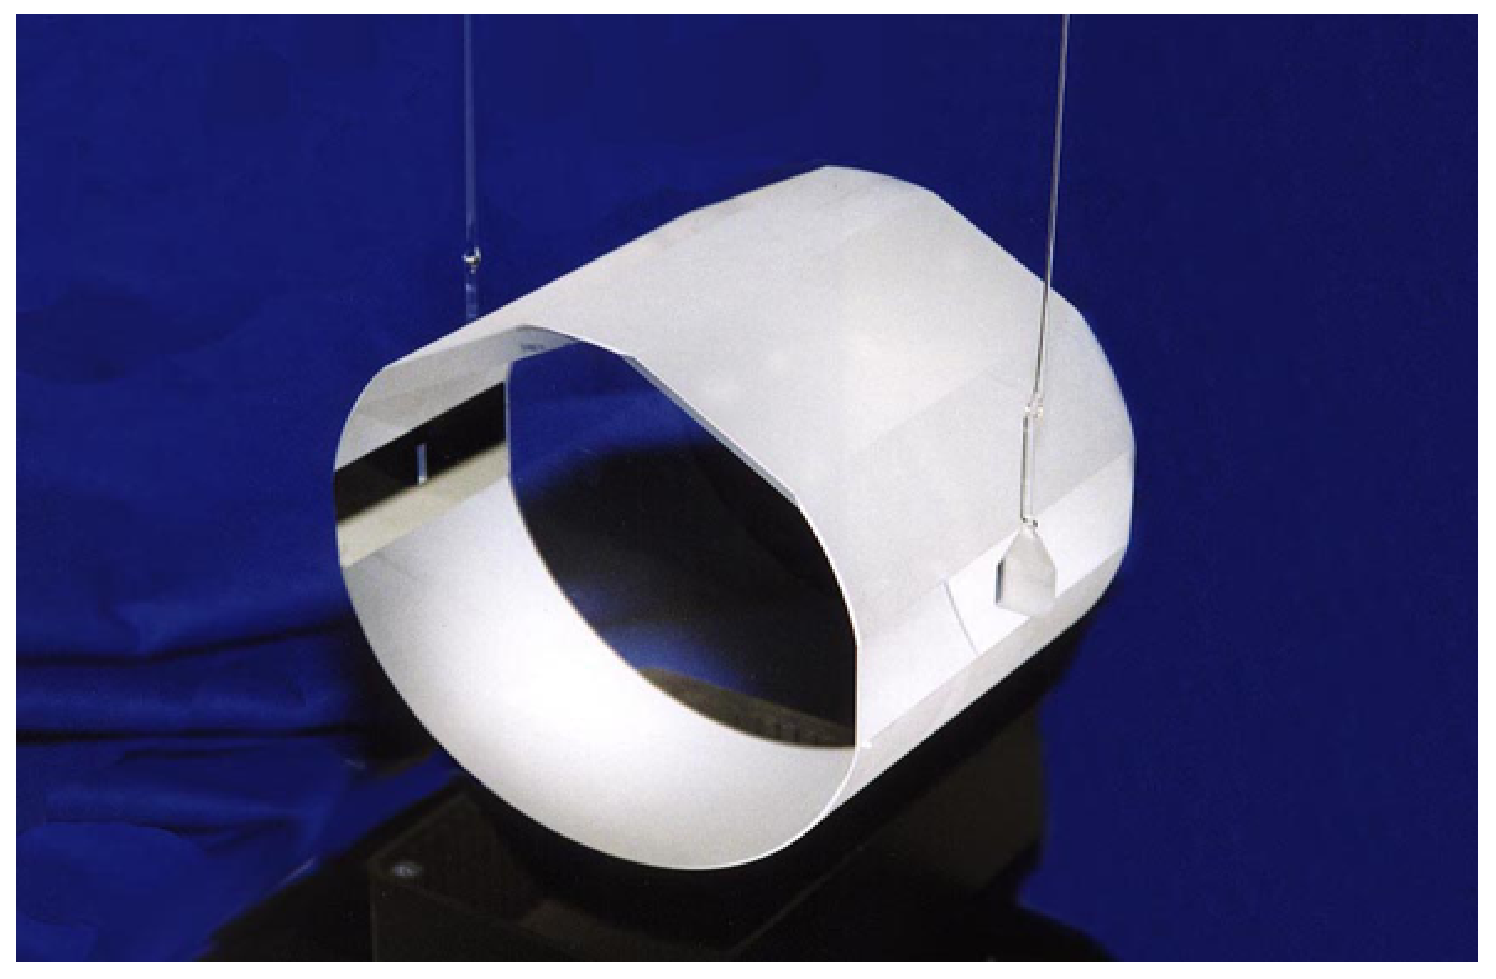
\includegraphics[scale=0.3]{fig4}}
  \caption{\it Prototype `monolithic' fused silica test mass
    suspension. The mass (3\protect~kg) here is of 12.5\protect~cm
    diameter. Note final suspension will use four fibres.}
  \label{figure:silicamass}
\end{figure}}



%%%%%%%%%%%%%%%%%%%%%%%%%%%%%%%%%%%%%%%%%%%%%%%%%%%%%%%%%%%%%%%%%%%%%%%%%%%%%%
%%%%%%%%%%%%%%%%%%%%%%%%%%%%%%%%%%%%%%%%%%%%%%%%%%%%%%%%%%%%%%%%%%%%%%%%%%%%%%



\subsection{Quantum Noise}
\label{subsection:quantumnoise}

Heisenberg Uncertainty - brief outline discussion

\subsubsection{Photoelectron Shot Noise}
\label{subsubsection:shotnoise}

For gravitational wave signals to be detected, the output of the
interferometer must be held at one of a number of possible points on
an interference fringe. An obvious point to choose is halfway up a
fringe since the change in photon number produced by a given
differential change in arm length is greatest at this point.  The
interferometer may be stabilised to this point by sensing any changes
in intensity at the interferometer output with a photodiode and
feeding the resulting signal back, with suitable phase, to a
transducer capable of changing the position of one of the
interferometer mirrors.  Information about changes in the length of
the interferometer arms can then be obtained by monitoring the signal
fed back to the transducer.

As mentioned earlier it is very important that the system used for
sensing the optical fringe movement on the output of the
interferometer can resolve strains in space of $2 \times
10^{-23}(\rm Hz)^{-1/2}$ or lower, or differences in the lengths of the
two arms of less than $10^{-19}{\rm \ m(\rm Hz)^{-1/2}}$, a minute
displacement compared to the wavelength of light $\simeq 10^{-6}$~m. A
limitation to the sensitivity of the optical readout scheme is set by
shot noise in the detected photocurrent. From consideration of the
number of photoelectrons (assumed to obey Poisson statistics) measured
in a time $\tau$ it can be shown~\cite{HoughMG5} that the detectable
strain sensitivity depends on the level of laser power $P$ of
wavelength $\lambda$ used to illuminate the interferometer of arm
length $L$, and on the time $\tau$, such that:
%
\begin{equation}
  {\rm detectable\ strain\ in\ time\ } \tau = \frac 1{L}\left[\frac{\lambda h
  c}{2 \pi^{2} P \tau}\right]^{1/2},
  \label{equation:shot1}
\end{equation}
%
or
%
\begin{equation}
  {\rm detectable\ strain\ }(\rm Hz)^{-1/2} = \frac
  1{L}\left[\frac{\lambda h c}{\pi^{2} P }\right]^{1/2},
  \label{equation:shot2}
\end{equation}
%
where $c$ is the velocity of light and $h$ is Planck's constant and we
assume that the photodetectors have a quantum efficiency $\simeq$
1. Thus achievement of the required strain sensitivity level requires
a laser, operating at a wavelength of $10^{-6}$~m, to provide $6
\times 10^{6}$~W power at the input to a simple Michelson
interferometer. This is a formidable requirement; however there are a
number of techniques which allow a large reduction in this power
requirement and these will be discussed in the next section.

%%%%%%%%%%%%%%%%%%%%%%%%%%%%%%%%%%%%%%%%%%%%%%%%%%%%%%%%%%%%%%%%%%%%%%%%%%%%%%

\subsubsection{Radiation Pressure Noise}
\label{subsubsection:radiationnoise}

Radiation pressure noise.  Ponderomotive squeezing/heavier test masses.

%%%%%%%%%%%%%%%%%%%%%%%%%%%%%%%%%%%%%%%%%%%%%%%%%%%%%%%%%%%%%%%%%%%%%%%%%%%%%%
%%%%%%%%%%%%%%%%%%%%%%%%%%%%%%%%%%%%%%%%%%%%%%%%%%%%%%%%%%%%%%%%%%%%%%%%%%%%%%


\newpage

\section{Laser Interferometric Techniques for Gravitational Wave Detectors}
\label{section:interferometry}

As explained in the preceding Section~\ref{subsection:shotnoise},
high power laser light is needed to overcome limitations of a
detector's sensitivity due to photoelectron shot noise. The situation
can be helped greatly if a multi-pass arrangement is used in the arms
of the interferometer as this multiplies up the apparent movement by
the number of bounces the light makes in the arms. The multiple beams
can either be separate as in an optical delay line~\cite{Weiss,
  Billing}, or may lie on top of each other as in a Fabry-Perot
resonant cavity~\cite{Drever2} as shown in
Fig.~\ref{figure:Michelsons}.

\epubtkImage{}{%
\begin{figure}[hptb]
  \centerline{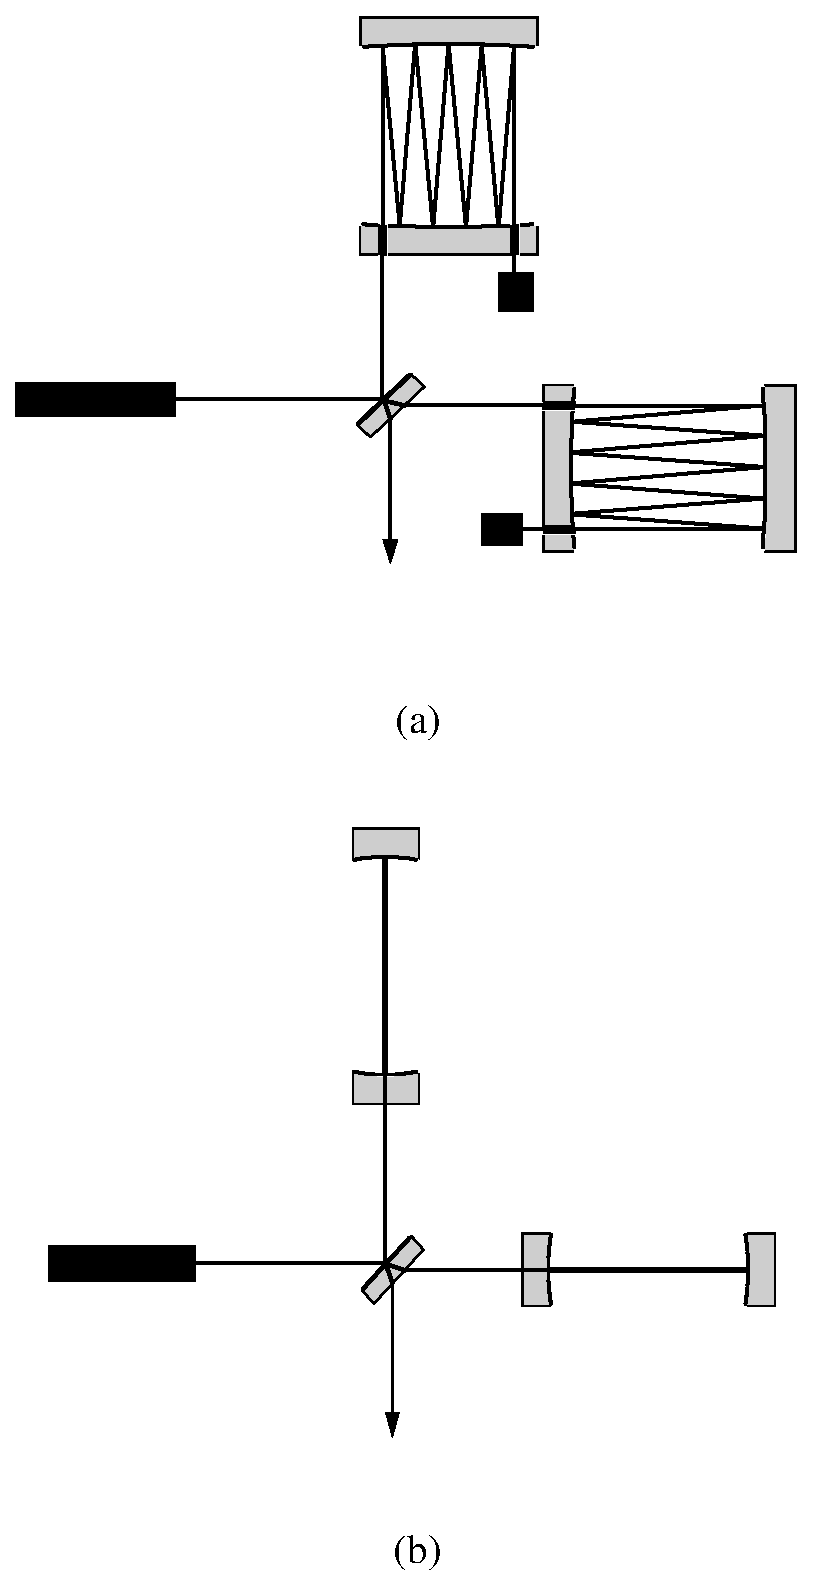
\includegraphics[scale=0.3]{fig5e}}
  \caption{\it Michelson interferometers with (a) delay lines and (b)
    Fabry-Perot cavities in the arms of the interferometer.}
  \label{figure:Michelsons}
\end{figure}}

Optimally, the light should be stored for a time comparable to the
characteristic timescale of the signal. Thus if signals of
characteristic timescale 1~msec are to be searched for, the number of
bounces should be approximately 50 for an arm length of 3~km. With 50
bounces the required laser power is reduced to $2.4 \times 10^3$~W,
still a formidable requirement.



%%%%%%%%%%%%%%%%%%%%%%%%%%%%%%%%%%%%%%%%%%%%%%%%%%%%%%%%%%%%%%%%%%%%%%%%%%%%%%%%
%%%
%%%%%%%%%%%%%%%%%%%%%%%%%%%%%%%%%%%%%%%%%%%%%%%%%%%%%%%%%%%%%%%%%%%%%%%%%%%%%%%%
%%%

\subsection{Power Recycling}
\label{subsection:powerrec}

It can be shown that optimum signal to noise ratio in a Michelson
interferometer can be obtained when the arm lengths are such that the
output light is very close to a minimum. (This is not intuitively
obvious and is discussed more fully in~\cite{Edelstein}). Thus rather
than lock the interferometer to the side of a fringe as discussed
above in Section~\ref{subsection:shotnoise}, it is usual to make use of a
modulation technique to operate the interferometer close to a null in
the interference pattern. An electro-optic phase modulator placed in
front of the interferometer can be used to phase modulate the input
laser light. If the arms of the interferometer are arranged to have a
slight mismatch in length this results in a detected signal which when
demodulated, is zero with the cavity exactly on a null fringe and
changes sign on different sides of the null providing a bipolar error
signal; this can be fed back to the transducer controlling the
interferometer mirror to hold the interferometer locked near to a null
fringe.

In this situation if the mirrors are of very low optical loss, nearly
all of the light supplied to the interferometer is reflected back
towards the laser. In other words the laser is not properly impedance
matched to the interferometer. The impedance matching can be improved
by placing another mirror of correctly chosen transmission -- a power
recycling mirror -- between the laser and the interferometer so that a
resonant cavity is formed between this mirror and the rest of the
interferometer; in the case of perfect impedance matching no light is
reflected back towards the laser~\cite{Drever3, Schilling}. There is
then a power build-up inside the interferometer. This can
be high enough to create the required kilowatts of laser light at the
beamsplitter, starting from an input laser light of only about 10~W.

To be more precise, if the main optical power losses are those
associated with the test mass mirrors -- taken to be A per reflection --
the intensity inside the whole system considered as one large cavity
is increased by a factor given by $(\pi L)/(c A \tau)$, where the
number of bounces, or light storage time, is optimised for signals of
timescale $\tau$ and the other symbols have their usual meaning. Then:
%
\begin{equation}
  {\rm detectable\ strain\ in\ time\ } \tau = \left( \frac{\lambda h
  A}{4 \pi L P \tau^2} \right)^{1/2}.
  \label{equation:shotpower}
\end{equation}

%%%%%%%%%%%%%%%%%%%%%%%%%%%%%%%%%%%%%%%%%%%%%%%%%%%%%%%%%%%%%%%%%%%%%%%%%%%%%%%%
%%%
%%%%%%%%%%%%%%%%%%%%%%%%%%%%%%%%%%%%%%%%%%%%%%%%%%%%%%%%%%%%%%%%%%%%%%%%%%%%%%%%
%%%

\subsection{Signal Recycling}
\label{subsection:sigrec}

To enhance further the sensitivity of an interferometric detector and
to allow some narrowing of the detection bandwidth, which may be
valuable in searches for continuous wave sources of gravitational
radiation, another technique known as signal recycling can be
implemented~\cite{Meers, Strain, Heinzel}. This relies on the fact
that sidebands created on the light by gravitational wave signals
interacting with the arms do not interfere destructively and so do
appear at the output of the interferometer. If a mirror of suitably
chosen reflectivity is put at the output of the system as shown in
Fig.~\ref{figure:Michelsons2}, then the sidebands can be recycled back
into the interferometer where they resonate, and hence the signal size
over a given bandwidth (set by the mirror reflectivity) is enhanced.

\epubtkImage{}{%
\begin{figure}[hptb]
  \centerline{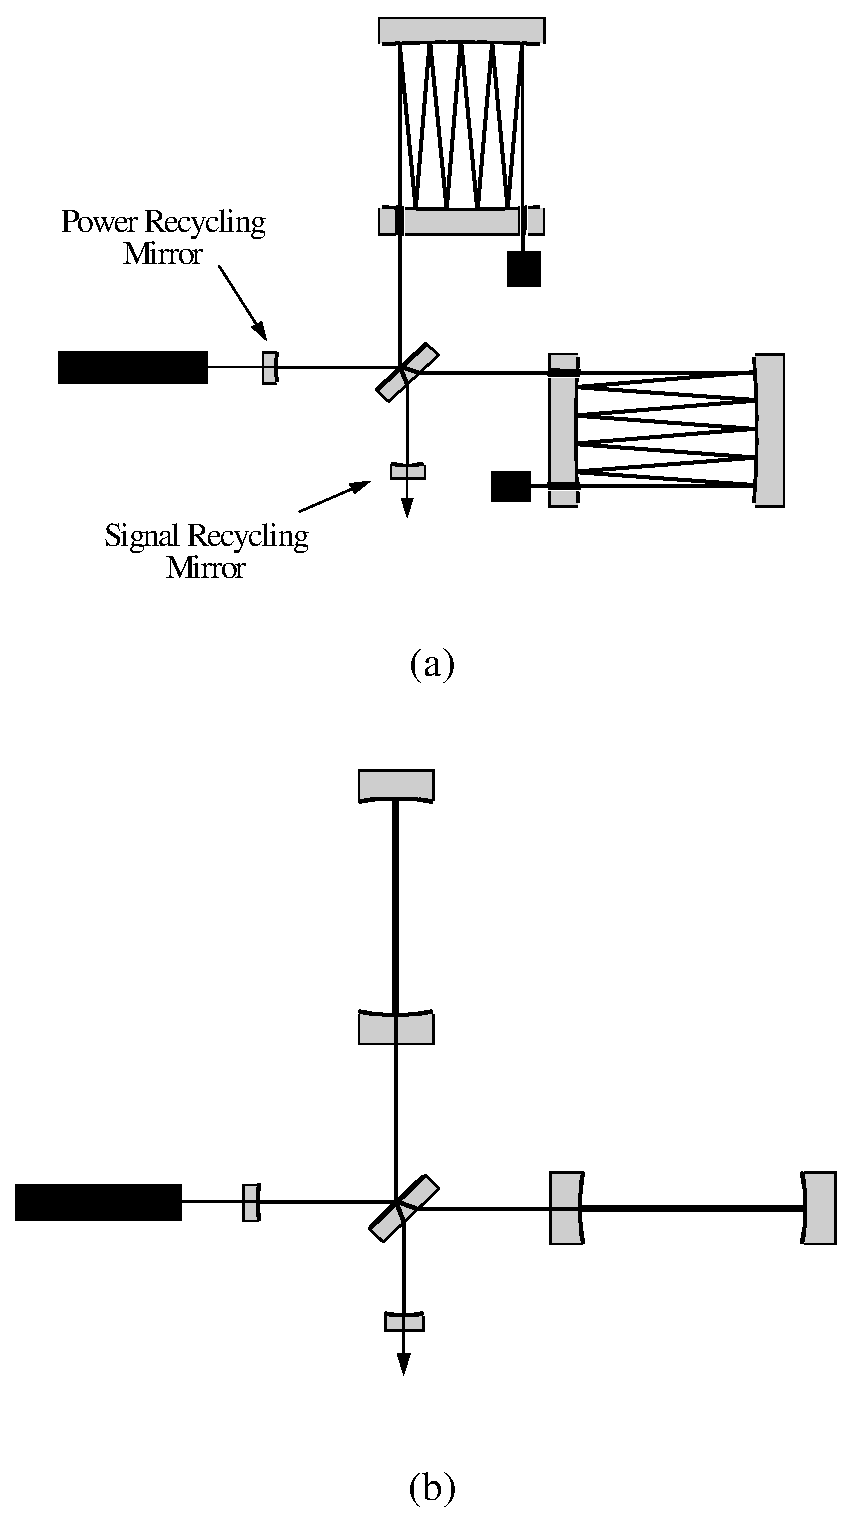
\includegraphics[scale=0.3]{fig6}}
  \caption{\it The implementation of power and signal recycling on the two
    interferometers shown in the previous figure,
    Fig.\protect~\protect\ref{figure:Michelsons}.}
  \label{figure:Michelsons2}
\end{figure}}

The centre of this frequency band is set by the precise length of the
cavity formed by the signal recycling mirror and the cavities in the
interferometer arms. Thus control of the precise position of the
signal recycling mirror allows tuning of the frequency at which the
performance is peaked.

Often signal recycling will be used to provide a narrow bandwidth to
search for continuous wave sources as mentioned above, however it may
also be used with a relatively broad bandwidth, centred away from
zero frequency, and this application is useful for matching the
frequency response of the detector to expected spectral densities of
certain broadband or ``chirping'' signals.

%%%%%%%%%%%%%%%%%%%%%%%%%%%%%%%%%%%%%%%%%%%%%%%%%%%%%%%%%%%%%%%%%%%%%%%%%%%%%%%%
%%%
%%%%%%%%%%%%%%%%%%%%%%%%%%%%%%%%%%%%%%%%%%%%%%%%%%%%%%%%%%%%%%%%%%%%%%%%%%%%%%%%
%%%

\subsection{Fluctuations in Radiation Pressure}
\label{subsection:radpress}

A phenomenon which becomes increasingly important as the effective
laser power in the arms is increased is the effect on the test masses
of fluctuations in the radiation pressure of the light in the
arms. From~\cite{Edelstein}, for a simple Michelson interferometer
with power $P/2$ in each arm, the power spectral density of the
fluctuating motion of the test mass $m$ induced by the fluctuations in
the radiation pressure at angular frequency $\omega$ is given by
%
\begin{equation}
  (\delta x^2(\omega)) = \left(\frac{4Ph}{m^2 \omega^{4} c
  \lambda}\right),
  \label{equation:radiation1}
\end{equation}
%
where $h$ is Planck's constant, $c$ is the speed of light and
$\lambda$ the wavelength of the laser light. In the case of systems
with cavities in the arms where the number of effective reflections is
approximately 50, fluctuations in the amplitude of the light arise
immediately after the beamsplitter where vacuum fluctuations enter
into the system. These are then enhanced by the power build up effects
of the optical cavities. In this case
%
\begin{equation}
  (\delta x^2(\omega)) = (50)^2 \times \left(\frac{4Ph}{m^2 \omega^{4} c
  \lambda}\right).
  \label{equation:radiation2}
\end{equation}
%
Evaluating this at 10~Hz, for powers of around $5 \times 10^3$~W
after the beamsplitter and masses of 30~kg, indicates an amplitude
spectral density for each mass of $9 \times 10^{-20} {\rm
\ m}(\rm Hz)^{-1/2}$. Given the target sensitivity of the detector at
10~Hz in Fig.~\ref{figure:LIGOsens} of approximately $7 \times
10^{-23}(\rm Hz)^{-1/2}$ which translates to a motion of each test mass
of close to $10^{-19} {\rm \ m}(\rm Hz)^{-1/2}$ it is clear that
radiation pressure may be a significant limitation at low
frequency. Of course the effects of the radiation pressure
fluctuations can be reduced by increasing the test masses, or by
decreasing the laser power at the expense of deproving sensitivity at
higher frequencies.

It should be noted that as discussed in~\cite{Edelstein, Caves1,
Caves2} and~\cite{Loudon} for a simple Michelson system,
the optimisation of laser power to minimise the combined effect photon
shot noise and radiation pressure fluctuations allows one to reach
exactly the sensitivity limit predicted by the Heisenberg Uncertainty
Principle, in its position and momentum formulation. An extension of
this analysis to a system with cavities in the arms has been carried
out by one of the authors~\cite{Houghprivcomm} with the same result
and it seems likely to be true for the more complicated optical
systems using power and signal recycling also.


%%%%%%%%%%%%%%%%%%%%%%%%%%%%%%%%%%%%%%%%%%%%%%%%%%%%%%%%%%%%%%%%%%%%%%

\subsection{Application of these Techniques}
\label{subsection:application}

Using appropriate optical configurations that employ power and signal
recycling as described above in ~\ref{subsection:powerrec} and
\ref{subsection:sigrec}, the required laser power may thus be reduced
to a level (in the range of 10 to 100~W) where laser sources are or
are becoming available; however stringent requirements on technical
noise must be satisfied.



%%%%%%%%%%%%%%%%%%%%%%%%%%%%%%%%%%%%%%%%%%%%%%%%%%%%%%%%%%%%%%%%%%%%%%%

\subsubsection{Technical noise requirements}
\label{subsubsection:lasernoise}

\begin{itemize}
\item {\bf Power fluctuations} \\
  As described above in Section~\ref{subsection:powerrec}
  gravitational wave interferometers are typically designed to operate
  with the length of the interferometer arms set such that the output
  of the interferometer is close to a minimum in the output light. If
  the interferometer were operated exactly at the null point in the
  fringe pattern, then in principle it would be insensitive to power
  fluctuations in the input laser light. However in practice there
  will be small offsets from the null position causing some
  sensitivity to this noise source.  In this case it can be
  shown~\cite{Hough} that the required power stability of the laser in
  the frequency range of interest for gravitational wave detection may
  be estimated to be
  %
  \begin{equation}
    \frac{\delta P}{P} \simeq h (\delta L/L)^{-1},
    \label{equation:intnoise1}
  \end{equation}
  %
  where $\delta P/P$ are the relative power fluctuations of the laser,
  and $\delta L$ is the offset from the null fringe position for an
  interferometer of arm length $L$.  From calculations of the effects
  of low frequency seismic noise for the initial designs of long
  baseline detector~\cite{Hough} it can be estimated that the rms
  motion will be of the order of $10^{-13}$~m when the system is
  operating. Taking strains of around $2 \times 10^{-24}(\rm
  Hz)^{-1/2}$ at 300~Hz, as shown in the lower curve in
  Fig.~\ref{figure:LIGOsens} for LIGO~2, as typical of that desired
  for upgraded detectors, requires power fluctuations of the laser not
  to exceed
  %
  \begin{equation}
    \frac{\delta P}{P} \leq 10^{-7} (\rm Hz)^{-1/2} \quad {\rm at}
    \simeq 300 {\rm \ Hz}.
    \label{equation:intnoise2}
  \end{equation}
  %
  To achieve this level of power fluctuations typically requires the
  use of active stabilisation techniques of the type developed for
  argon ion lasers~\cite{Mangan}.
%
\item {\bf Frequency fluctuations} \\
  For a simple Michelson interferometer it can be shown that a change
  $\delta x$ in the differential path length, $x$, of the
  interferometer arms causes a phase change $\delta \phi$ in the light
  at the interferometer output given by $\delta \phi = (2\pi/c) (\nu
  \delta x + x \delta\nu)$ where $\delta \nu$ is a change in the laser
  frequency $\nu$ and $c$ is the speed of light. It follows From that if
  the lengths of the interferometer arms are exactly equal (i.~e. $x =
  0$), the interferometer output is insensitive to fluctuations in the
  frequency of the input laser light, provided that, in the case of
  Fabry-Perot cavities in the arms, the fluctuations are not so great
  that the cavities cannot remain on resonance.  In practice however,
  differences in the optical properties of the interferometer mirrors
  result in  slightly different effective arm lengths, a difference of
  perhaps a few tens of metres. Then the relationship between thelimit
  to detectable gravitational wave amplitude and the fluctuations
  $d\nu$ of the laser frequency $\nu$ is given by~\cite{Hough}
  %
  \begin{equation}
    \frac{\delta \nu}{\nu} \simeq h(x/L)^{-1}.
    \label{equation:frequnoise}
  \end{equation}
  %
  Hence to achieve the target sensitivity used in the above calculation
  using a detector with arms of length 4~km, maximal fractional
  frequency fluctuations of
  %
  \begin{equation}
    \frac{\delta \nu}{\nu} \leq 10^{-21}(\rm Hz)^{-1/2}.
    \label{equation:freqspecification}
  \end{equation}
  %
  are required.This level of frequency noise may be achieved by the use of
  appropriate laser frequency stabilisation systems involving high
  finesse reference cavities~\cite{Hough}.

  Although the calculation here is for a simple Michelson
  interferometer, similar arguments apply to the more sophisticated
  systems with arm cavities, power recycling and signal recycling
  discussed earlier and lead to the same conclusions.

\item {\bf Beam geometry fluctuations} \\
  Fluctuations in the lateral or angular position of the input laser
  beam, along with changes in its size and variations in its
  phasefront curvature may all couple into the output signal of an
  interferometer and reduce its sensitivity. These fluctuations may be
  due to intrinsic laser mechanical noise (from water cooling for
  example) or from seismic motion of the laser with respect to the
  isolated test masses. As an example of their importance,
  fluctuations in the lateral position of the beam may couple into
  interferometer measurements through a misalignment of the
  beamsplitter with respect to the interferometer mirrors. A lateral
  movement $\delta z$ of the beam incident on the beamsplitter,
  coupled with an angular misalignment of the beamsplitter of
  $\alpha/2$ results in a phase mismatch $\delta \phi$ of the
  interfering beams, such that~\cite{Rudiger}
  %
  \begin{equation}
    \delta \phi = (4 \pi/\lambda) \alpha \delta z.
    \label{equation:beamgeomfluc}
  \end{equation}
  %
  A typical beamsplitter misalignment of $\simeq 10^{-7}$
  radians means that to achieve sensitivities of the level described
  above using a detector with 3 or 4~km arms, and 50 bounces of the
  light in each arm, a level of beam geometry fluctuations at the
  beamsplitter of close to $10^{-12}{\rm \ m}(\rm Hz)^{-1/2}$ at
  300~Hz is required.

  Typically, and ignoring possible ameliorating effects of the power
  recycling cavity on beam geometry fluctuations, this will mean that
  the beam positional fluctuations of the laser need to be suppressed
  by several orders of magnitude. The two main methods of reducing
  beam geometry fluctuations are 1) passing the input beam through a
  single mode optical fibre~\cite{Meersphd} and 2) using a resonant
  cavity as a modecleaner~\cite{Rudiger, Skeldon, Willke, Araya}.

  Passing the beam through a single mode optical fibre helps to
  eliminate beam geometry fluctuations, as deviations of the beam from
  a Gaussian TEM00 mode are equivalent to higher order spatial modes,
  which are thus attenuated by the optical fibre.  However there are
  limitations to the use of optical fibres mainly due to the limited
  power handling capacity of the fibres; care must also be taken to
  avoid introducing extra beam geometry fluctuations from movements of
  the fibre itself.

  A cavity may be used to reduce beam geometry fluctuations if it is
  adjusted to be resonant only for the TEM00 mode of the input light.
  Any higher order modes should thus be suppressed~\cite{Rudiger}.
  The use of a resonant cavity should allow the handling of higher
  laser powers and has the additional benefits of acting as
  a filter for fast fluctuations in laser frequency and
  power~\cite{Skeldon, Willke}. This latter property is extremely
  useful for the conditioning of the light from some laser sources as
  will be discussed below.
\end{itemize}



%%%%%%%%%%%%%%%%%%%%%%%%%%%%%%%%%%%%%%%%%%%%%%%%%%%%%%%%%%%%%%%%%%%%%%%%%%%%%%%%
%%%

\subsubsection{Laser design}
\label{subsubsection:laserdesign}

From Equation~(\ref{equation:shot1}) it can be seen that the
photon-noise limited sensitivity of an interferometer is proportional
to $P^{-1/2}$ where $P$ is the laser power incident on the
interferometer, and $\lambda^{1/2}$ where $\lambda$ is the wavelength
of the laser light. Thus single frequency lasers of high output power
and short wavelength are desirable. With these constraints in mind,
laser development has concentrated on argon-ion lasers and Nd:YAG
lasers.  Argon-ion lasers emitting light at 514~nm have been used to
illuminate several interferometric gravitational wave detector
prototypes, see for example~\cite{Shoemaker, Robertson}. They have an
output power in the required single spatial (TEM00q) mode of operation
typically of around several Watts, sufficient for this type of laser
to have been proposed as the initial laser for a full-scale
interferometric detector~\cite{Vogt}. For advanced detectors higher
laser powers would be desirable and it has been demonstrated that the
output of several argon-ion lasers could be coherently added for this
purpose~\cite{Kerr}. However the disadvantages of argon-ion lasers
include the increased optical absorption and damage, and more
pronounced effects due to scattering, for light of this shorter
wavelength. In addition argon-ion lasers are relatively inefficient.

Nd:YAG lasers, emitting at 1064~nm or frequency doubled to 532~nm,
present an alternative. The longer wavelength is less desirable than
the 514~nm of the argon-laser, as more laser power is needed to obtain
the same sensitivity; in addition, the resulting increase in beam
diameter leads to a need for larger optical components. For example in
an optical cavity the diameter of the beam at any point is
proportional to the square root of the wavelength~\cite{Kogelnik} and
to keep diffractive losses at each test mass below $1 \times 10^{-6}$
it can be shown that the diameter of each test mass must be greater
than 2.6~times the beam diameter at the test mass. Thus the test
masses for gravitational wave detectors have to be 1.4 times larger in
diameter for infrared than for green light. Nd:YAG sources do however
have some compelling advantages, and in particular the potential for
scaling Nd:YAG laser designs up to levels of 100~W or
more~\cite{Shine} combined with their superior efficiency, has led all
the long baseline interferometer projects to choose some form of
Nd:YAG light source.

Compact sources of lower powers of Nd:YAG light have been available
for several years in the form of monolithic diode-pumped ring
lasers~\cite{Kane1}.  Investigations have shown that the technical
noise associated with these lasers may be well controlled and reduced
to levels comparable to those needed for gravitational wave
interferometer sources~\cite{Kane2, Fritschel, Campbell, Rowan4,
Harb}. Different approaches to obtaining high powers of low-noise
Nd:YAG light have been studied. They all have in common the
use of a stable lower power laser as a master oscillator.

One approach is to use a lower power Nd:YAG master oscillator to
injection lock a higher power Nd:YAG slave laser, with the length of
the slave laser cavity being locked to the frequency of the light from
the master oscillator~\cite{Cregut, Nabors, Golla}. Up to 20~W of
single frequency laser light have been obtained using this
method~\cite{Shine}, which has the desirable feature that the higher
power slave laser light has noise properties which are for the most
part dominated by those of the master laser light~\cite{Farinas}. This
is desirable since it is typically easier to apply active noise
reduction techniques to stabilise the lower power master lasers.
Injection locked systems of this type are being developed for use by
the Virgo, TAMA~300 and GEO~600 projects, each of which requires
$\simeq$~10~W of laser light for initial operation.

However to adapt this technique for producing still higher powers from
the slave laser requires care, since the light power needed from the
master oscillator also increases. To meet this requirement systems
have been proposed in which a series of lasers are successively
injection locked.

An alternative scheme has been developed for use by the LIGO
project~\cite{Weichmann}. Light from a master laser is passed through
diode-pumped Nd:YAG amplification stages in a master oscillator/power
amplifier (MOPA) configuration. This approach has the advantage of
allowing a very high continuous light power to be
obtained using multiple amplification stages, without the need for
multiple cavity locking schemes.  However the
effects of this design configuration on the noise properties of the
amplified light must be addressed.

In particular, to obtain high performance from the modulation
techniques discussed in section~\ref{subsection:powerrec} it is
necessary that at the modulation frequency, the power fluctuations of
the laser light used must be shot noise limited in the amount of light
detected at the interferometer output (typically up to a few Watts).

Previous studies of the noise properties of optical amplifiers have
shown that in a given output power of light from an optical amplifier,
power fluctuations exist which are in excess of those obtained from a
shot noise limited laser of the same output power~\cite{Harris}. This
gain dependent excess noise arises from the beating of the spontaneous
emission from the amplifier with the light being amplified.
Measurements of this excess noise at RF modulation frequencies have
been made using a free space Nd:YAG linear optical amplifier
system~\cite{Tulloch}. For this type of light source to be suitable
for use in an interferometric gravitational wave detector, it is
necessary to reduce these high frequency power fluctuations; a
suitable technique is to pass the light through a resonant cavity
similar to that used to spatially filter the input laser light as
described in section~\ref{subsubsection:lasernoise}~\cite{Willke}. Above
the corner frequency $f_{c}$ of the cavity, power and frequency
fluctuations of the laser light are reduced by a factor $f/ f_{c}$
where $f$ is the frequency at which the fluctuation occurs, and
%
\begin{equation}
  f_c = \frac{({\rm cavity\ free\ spectral\ range})}{(2 \times {\rm
  \ finesse})}.
  \label{equation:filtering}
\end{equation}
%
Thus the excess power noise introduced by the amplification process
may be reduced to an appropriate level. The noise properties of
saturated free space Nd:YAG optical amplifiers remain to be
experimentally evaluated.

As mentioned earlier, a light source with the potential to combine the
increased efficiency of solid state lasers with the advantage of using
shorter wavelength light is a frequency doubled Nd:YAG laser.
While single frequency powers in excess of 10~W are obtainable,
sources of frequency-controllable doubled light of
an acceptable power level have still to be proven in terms of long term
reliability, but are likely to become available in the future.

%%%%%%%%%%%%%%%%%%%%%%%%%%%%%%%%%%%%%%%%%%%%%%%%%%%%%%%%%%%%%%%%%%%%%%%%%%%%%%%%
%%%
%%%%%%%%%%%%%%%%%%%%%%%%%%%%%%%%%%%%%%%%%%%%%%%%%%%%%%%%%%%%%%%%%%%%%%%%%%%%%%%%
%%%
%%%%%%%%%%%%%%%%%%%%%%%%%%%%%%%%%%%%%%%%%%%%%%%%%%%%%%%%%%%%%%%%%%%%%%%%%%%%%%%%
%%%

\newpage

\section{Operation of First Generation Long Baseline Detectors}
\label{section:construction}

Prior to the start of the 21$^{\rm st}$ Century there existed several prototype
laser interferometric detectors, constructed by various research groups around
the world -- at the Max-Planck-Instit\"ut f\"ur Quantenoptik in
Garching~\cite{Shoemaker}, at the University of Glasgow~\cite{Robertson}, at the
California Institute of Technology~\cite{Abramovici}, at the Massachusetts
Institute of Technology~\cite{Fritschel2}, at the Institute of Space and
Astronautical Science in Tokyo~\cite{Mizuno} and at the astronomical observatory
in Tokyo~\cite{Araya}. These detectors had arm lengths varying from 10~m to
100~m and had either multibeam delay lines or resonant Fabry-Perot cavities in
their arms.  The 10~m detector that used to exist at Glasgow is shown in
Fig.~\ref{figure:Glasgowprototype}.

\epubtkImage{}{%
\begin{figure}[hptb]
  \centerline{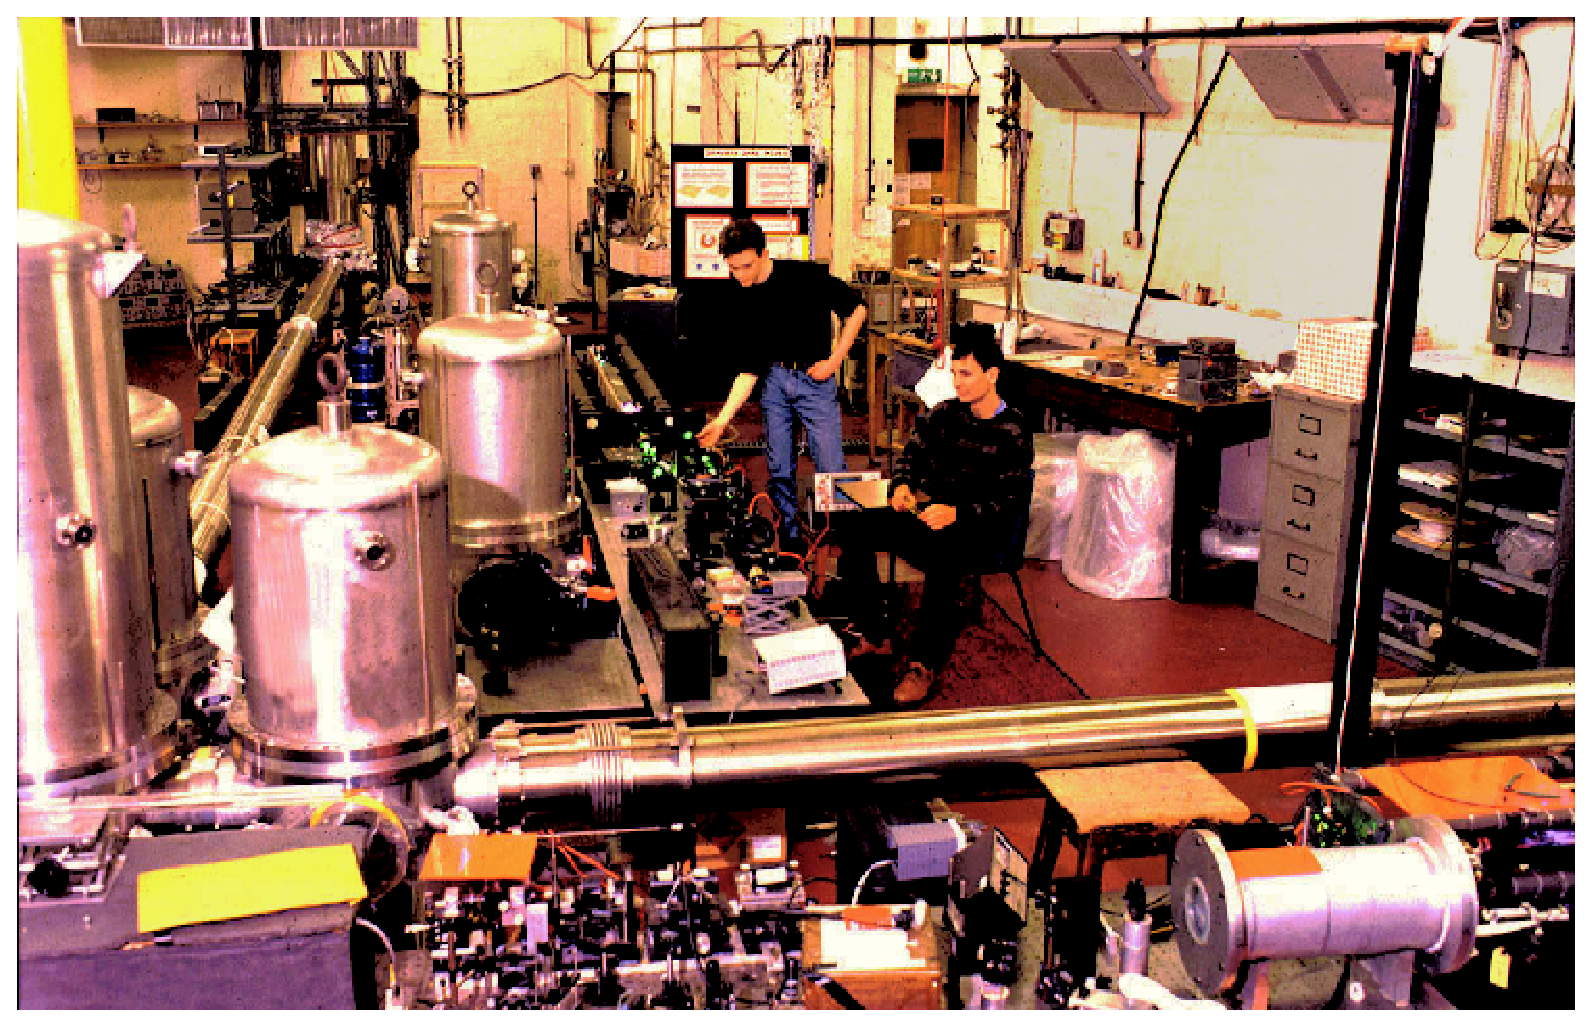
\includegraphics[scale=0.4]{figpro}}
  \caption{\it The 10~m prototype gravitational wave detector
    at Glasgow.}
  \label{figure:Glasgowprototype}
\end{figure}}

The sensitivities of some of these detectors reached a level -- better than
$10^{-18}$ for millisecond bursts -- such that the technology could be
considered sufficiently mature to propose the construction of detectors of much
longer baseline that would be capable of reaching the performance required to
have a real possibility of detecting gravitational waves.  An international
network of such long baseline gravitational wave detectors has now been
constructed and commissioned, and science quality data from these has been
produced and analysed since 2002 (see \S\ref{subsection:runs} and
\S\ref{subsection:results} for a review of recent science data runs and results).

The American LIGO project \cite{LIGOweb} comprises two detector
systems with arms of 4~km length, one in Hanford, Washington State, and one in
Livingston, Louisiana (also known as the LIGO Hanford Observatory 4k [LHO 4k] 
and LIGO Livingston Observatory 4k [LLO 4k], or H1 and L1
respectively). One half length, 2~km, interferometer was also contained inside
the same evacuated enclosure at Hanford (also known as the LHO 2k, or H2). The
design goal of the 4~km interferometers was to have a peak strain sensitivity
between 100--200~Hz of $\sim 3\times10^{-23}\,{\rm Hz}^{-1/2}$ \cite{LIGOSRD}
(see Fig.~\ref{figure:LIGOstrains}), which was achieved during the fifth 
science run (\S\ref{subsection:runs}). A birds-eye view of the Hanford site
showing the central building and the directions of the two arms is shown in
Fig.~\ref{figure:LIGOsite}. In October 2010 the LIGO detectors shut down and
decommissioning began in preparation for the installation of a more sensitive 
instrument known as Advanced LIGO (see \S\ref{subsection:aligo}).

\epubtkImage{}{%
\begin{figure}[hptb]
  \centerline{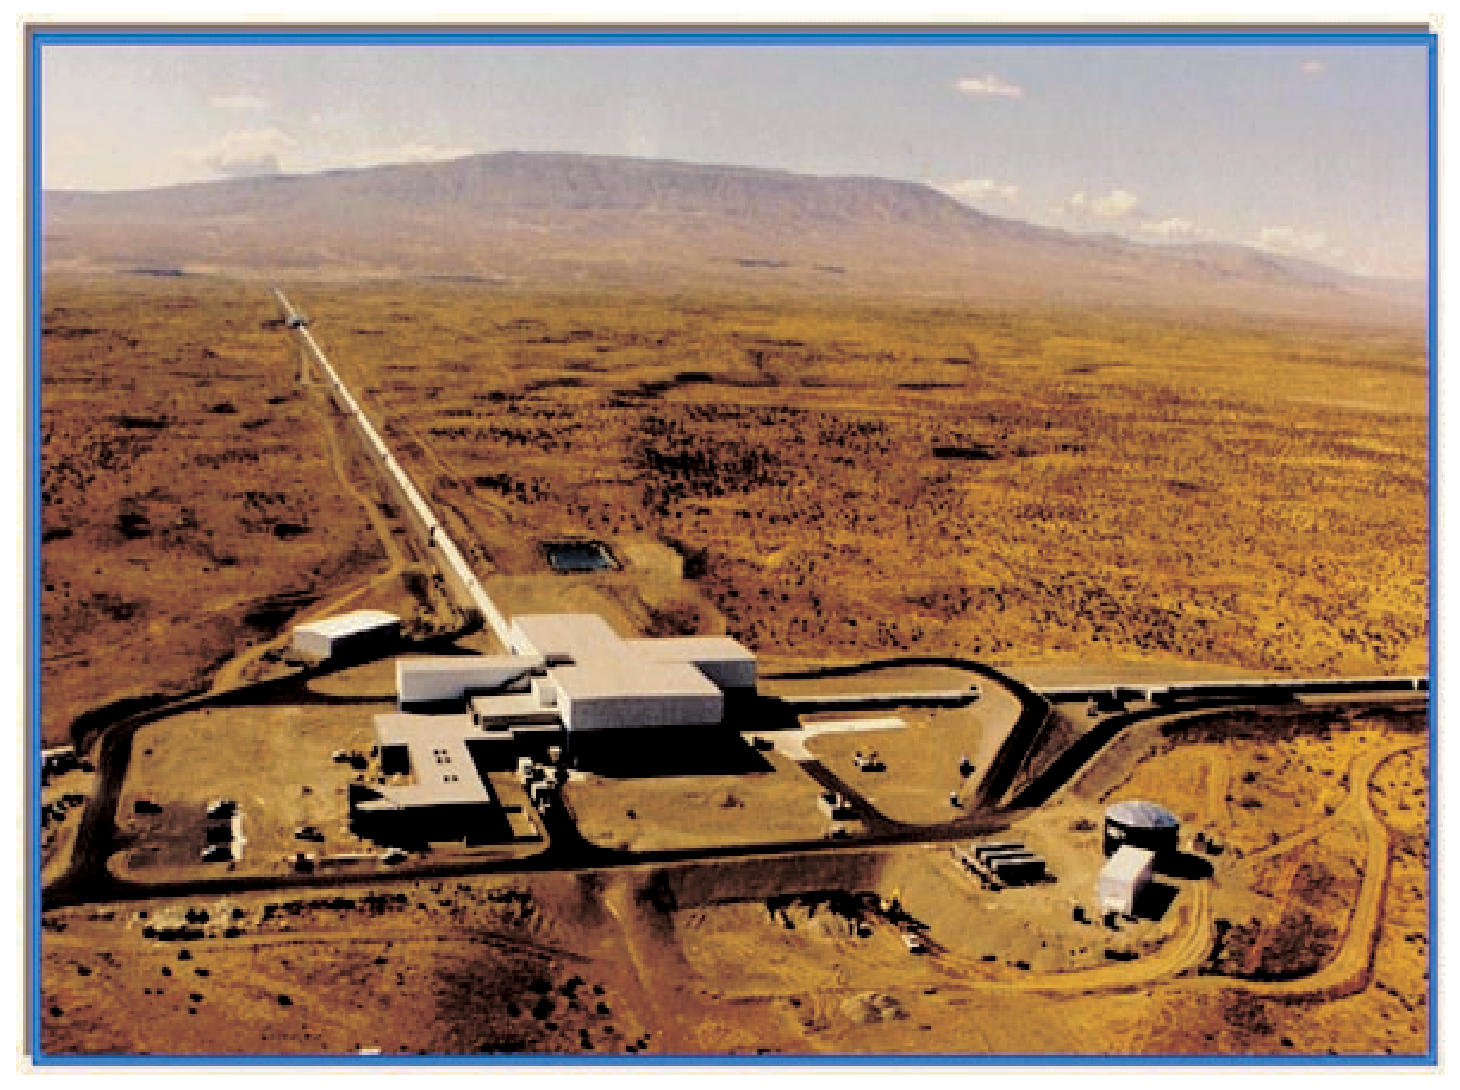
\includegraphics[scale=0.45]{fig7}}
  \caption{\it A bird's eye view of the LIGO detector, sited in
    Hanford, Washington State.}
  \label{figure:LIGOsite}
\end{figure}}

The French/Italian Virgo project \cite{Virgoweb} comprises a single 3~km arm
length detector at Cascina near Pisa. As mentioned earlier it is designed to
have better performance down to 10~Hz than the other detectors.

The TAMA~300 detector \cite{TAMAweb}, which has arms of length 300~m, at the
Tokyo Astronomical Observatory was the first of the ``beyond-prototype'' detectors
to become operational. This detector is built mainly underground and partly has
the aim of adding to the gravitational wave detector network for sensitivity to
events within the local group of galaxies, but is primarily a test bed for 
developing techniques for future larger scale detectors. Initial operation of
the interferometer was achieved in 1999 and power recycling was implemented for
data taking in 2003~\cite{Arai:2003}.

All the systems mentioned above are designed to use resonant cavities in the
arms of the detectors and use standard wire sling techniques for suspending the
test masses. The German/British detector, GEO~600 \cite{GEOweb}, built near
Hannover, Germany, is somewhat different. It makes use of a four pass delay line
system with advanced optical signal enhancement techniques, utilises very low
loss fused silica suspensions for the test masses, and despite its smaller size 
was designed to have a
sensitivity at frequencies above a few hundred Hz comparable to the first phases
of Virgo and LIGO during their initial operation. It uses both power
recycling and tunable signal recycling, often referred to together as dual
recycling.

To gain the most out of the detectors as a true network data sharing and joint
analyses are required. In the summer of 2001 the LIGO and GEO~600 teams signed a
Memorandum of Understanding (MoU), under the auspices of the LIGO Scientific
Collaboration (LSC) \cite{LSCweb}, allowing complete data sharing between the
two groups. Part of this agreement has been to ensure that both the LIGO and
GEO~600 have taken data in coincidence (see below). Coincident data taking,
and joint analysis, has also occurred between the TAMA~300 project and the LSC
detectors. The Virgo collaboration also signed a MoU with the LSC, which 
has allowed data sharing since May 2006.

The operation and commissioning of these detectors is a continually evolving 
process, and the current state of this review only covers developments until late-2010.
For the most up-to-date information on detectors readers are advised to consult
the proceedings of the Amaldi meetings, GWDAW (Gravitational Wave Data Analysis
Workshops), and GWADW (Gravitational Wave Advanced Detectors Workshops) -- see 
\cite{confs} for a list of past conferences.

For the first and second generations of detector much effort has gone into estimating
the expected number of sources that might be observable given their design
sensitivities. In particular, for what are
though to be the strongest sources: the coalescence of binary neutron stars or black 
holes (see \S\ref{sec:cbc} for current rates as constrained by observations). These 
estimates, based on observation and simulation, are summarised in \cite{Abadie:2010e}
and suggest initial detectors might expect to see 0.02, 0.004 and 0.007 events per 
year for binary neutron star, black hole-neutron star, and binary black hole systems
respectively (although there is a wide range covering orders of magnitude in these
estimates)\footnote{In terms of event rates the current best 
estimates for binary neutron
star merger rates, based on the known population of binary neutron star systems,
gives a 95\% confidence interval between 1--1000$\times10^{-6}$ per year per 
Milky Way Equivalent Galaxy (MWEG), where MWEG is equivalent to a volume that contains a blue
light luminosity with $L = 9\times10^9L_{\odot}$ (MWEG was used in
the S1 and S2 LIGO search, but was then changed to the $L_{10}$ unit, where $L_{10}$ is
given as $10^{10}$ times the blue light luminosity of the sun, although
there is only a 10\% difference between the two), \cite{Abadie:2010e, 
Kalogera:2004a, Kalogera:2004b}, with a peak in the distribution
at $100\times10^{-6}$ per year per MWEG -- or $\approx 0.02$ per year for initial 
LIGO at design sensitivity. The expected rate
of binary black hole systems, or black hole-neutron star systems is far harder
to infer as none have been observed, but estimates can be made on the population
for a wide variety of models and give a 95\% confidence range of
0.05--100$\times10^{-6}$ per year per MWEG and 0.01--30$\times10^{-6}$ per year per MWEG
respectively \cite{Abadie:2010e, OShaughnessy:2005, OShaughnessy:2008, Abbott:2008a}.
As an example of how to convert from rates to event numbers, cumulative blue light 
luminosities with respect to distance from the Earth in
Mpcs, and the horizon distances of the LIGO detectors from S2 through to S4,
can be seen in Figure 3 of \cite{Abbott:2008a}.}. Second generation detectors 
(see \S\ref{subsection:aligo}), which can observe approximately 
1000 time more volume than the initial detectors might expect to see 40, 10, and 20
per year for the same sources. With such rates a great deal of astrophysics could be
possible (see \cite{Sathyaprakash:2009} for examples).

\subsection{Science Runs}\label{subsection:runs}
Over the last decade the commissioning and improvement of the various gravitational 
wave detectors has been suspended at various stages to take data for
astrophysical analysis. These have been times when it was considered that the 
detectors were sensitive and stable enough (or had made sufficient improvements
over earlier states) to make astrophysical searches worthwhile. Within the LSC 
these have been called the {\it Science} (S) runs, for Virgo they have been the 
{\it Virgo Science Runs} (VSR), and for TAMA~300 they have been the {\it Data 
Taking} (DT) periods. A time-line of science runs for the various interferometric 
detectors, can be seen in Fig.~\ref{figure:runtimes}.

\epubtkImage{}{%
\begin{figure}[hptb]
  \centerline{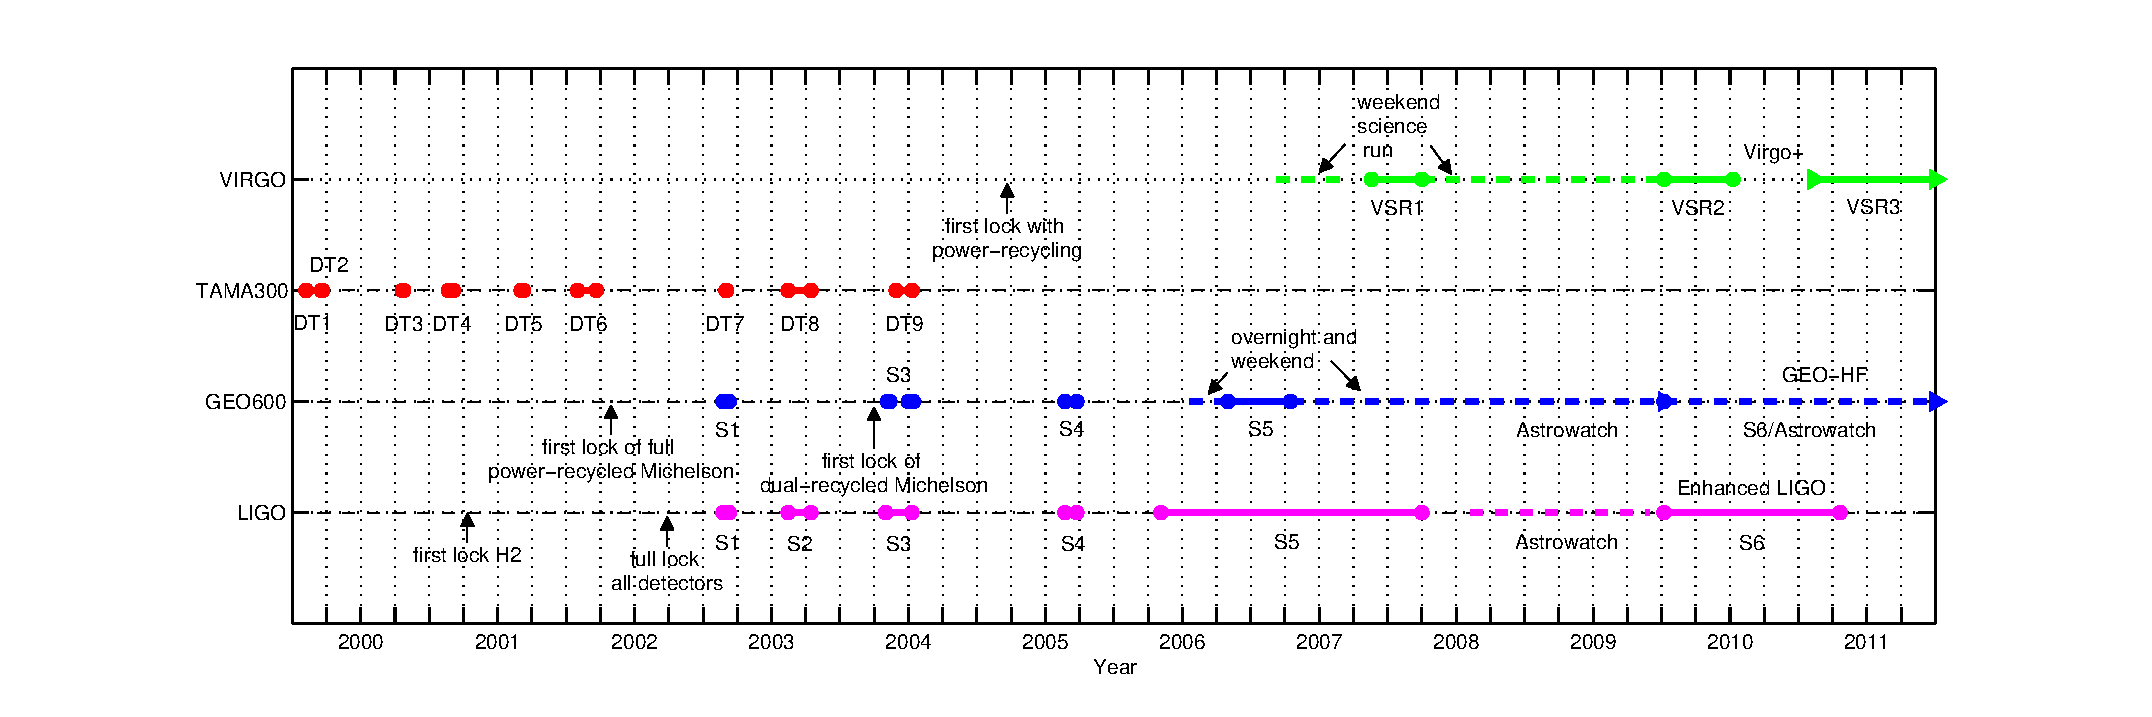
\includegraphics[scale=0.45]{runtimes}}
  \caption{\it A time-line of the science runs of the first generation
interferometric gravitational wave detectors, from their first lock to 
mid-2011.}
  \label{figure:runtimes}
\end{figure}}

A figure of merit for the sensitivity of a detector is to calculate its {\it 
horizon distance}. This is the maximum 
range out to which it could see the coalescence of two 1.4\,M$_{\odot}$ neutron 
stars that are optimally oriented and located (i.e.~with the orbital plane 
perpendicular to the line-of-sight, and with this plane parallel to the detector
plane, so that the antenna response is at its maximum) at a signal-to-noise ratio 
of 8 \cite{Abbott:2005b}. The horizon distance can be converted to a range that is an 
average over all sky locations and source orientations (i.e.~not the best 
case scenario) by dividing it by 2.26 \cite{Sutton:2003}) -- we shall use this angle 
averaged range throughout the rest of this review.

\subsubsection{TAMA~300}
The first interferometric detector to start regular data taking with sufficient
sensitivity and stability to enable it to potentially detect gravitational waves from the the galactic
centre was TAMA~300 \cite{Ando:2001}. Over the period between August 1999 to
January 2004 TAMA had nine data taking periods (denominated DT1--9) over which
time its typical strain noise sensitivity, in its most sensitive frequency band
improved from $\sim3\times10^{-19}\,{\rm Hz}^{-1/2}$ to
$\sim1.5\times10^{-21}\,{\rm Hz}^{-1/2}$ \cite{Akutsu:2006}.  TAMA~300 operated 
in coincidence with the LIGO and GEO~600 detectors for two of the science data 
taking periods. More recently focus has shifted to the Cryogenic Laser 
Interferometer Observatory (CLIO) prototype detector \cite{Yamamoto:2008, 
CLIOweb} designed to test technologies for a future {\it second generation} Japanese detector
called the Large-scale Cryogenic Gravitational-Wave Telescope (LCGT) 
(see \S\ref{subsection:aligo}).

\subsubsection{LIGO}\label{sec:ligoruns}
The first LIGO detector to achieve lock (meaning having the interferometer stably 
held on a dark fringe of the interference pattern, with light resonating throughout 
the cavity) was H2 in late 2000.
By early 2002 all three detectors had achieved lock and have since
undergone many periods of commissioning and science data taking. Over the period
between mid-2001 to mid 2002 the commissioning process improved the detectors'
peak sensitivities by several orders of magnitude, with L1 going from
$\sim10^{-17}-10^{-20}\,{\rm Hz}^{-1/2}$ at 150~Hz. In summer 2002 it was
decided that the detectors were at a sensitivity, and had a good enough lock
stability, to allow a science data taking run. This was potentially sensitive to
local galactic burst events. From 23 August to 9 September 2002 the three LIGO
detectors, along with GEO~600 (and, for some time, TAMA~300), undertook their
first coincident science run, denoted S1 (see \cite{Abbott:2004a} for the state
of the LIGO and GEO~600 detectors at the time of S1). At this time the most
sensitive detector was L1 with a peak sensitivity at around 300~Hz of
$2-3\times10^{-21}\,{\rm Hz}^{-1/2}$. The best strain amplitude sensitivity
curve for S1 (and the subsequent LIGO science runs) can be seen in
Fig.~\ref{figure:LIGOstrains}. The amount of time over the run that the
detectors were said to be in science mode, i.e. stable and with the
interferometer locked, called their duty cycle, or duty factor, was 42\% for L1,
58\% for H1 and 73\% for H2. . For the most sensitive detector, L1, the 
inspiral range was typically 0.08\,Mpc.

% LIGO S1 through S5 best strain sensitivities
\epubtkImage{}{%
\begin{figure}[hptb]
  \centerline{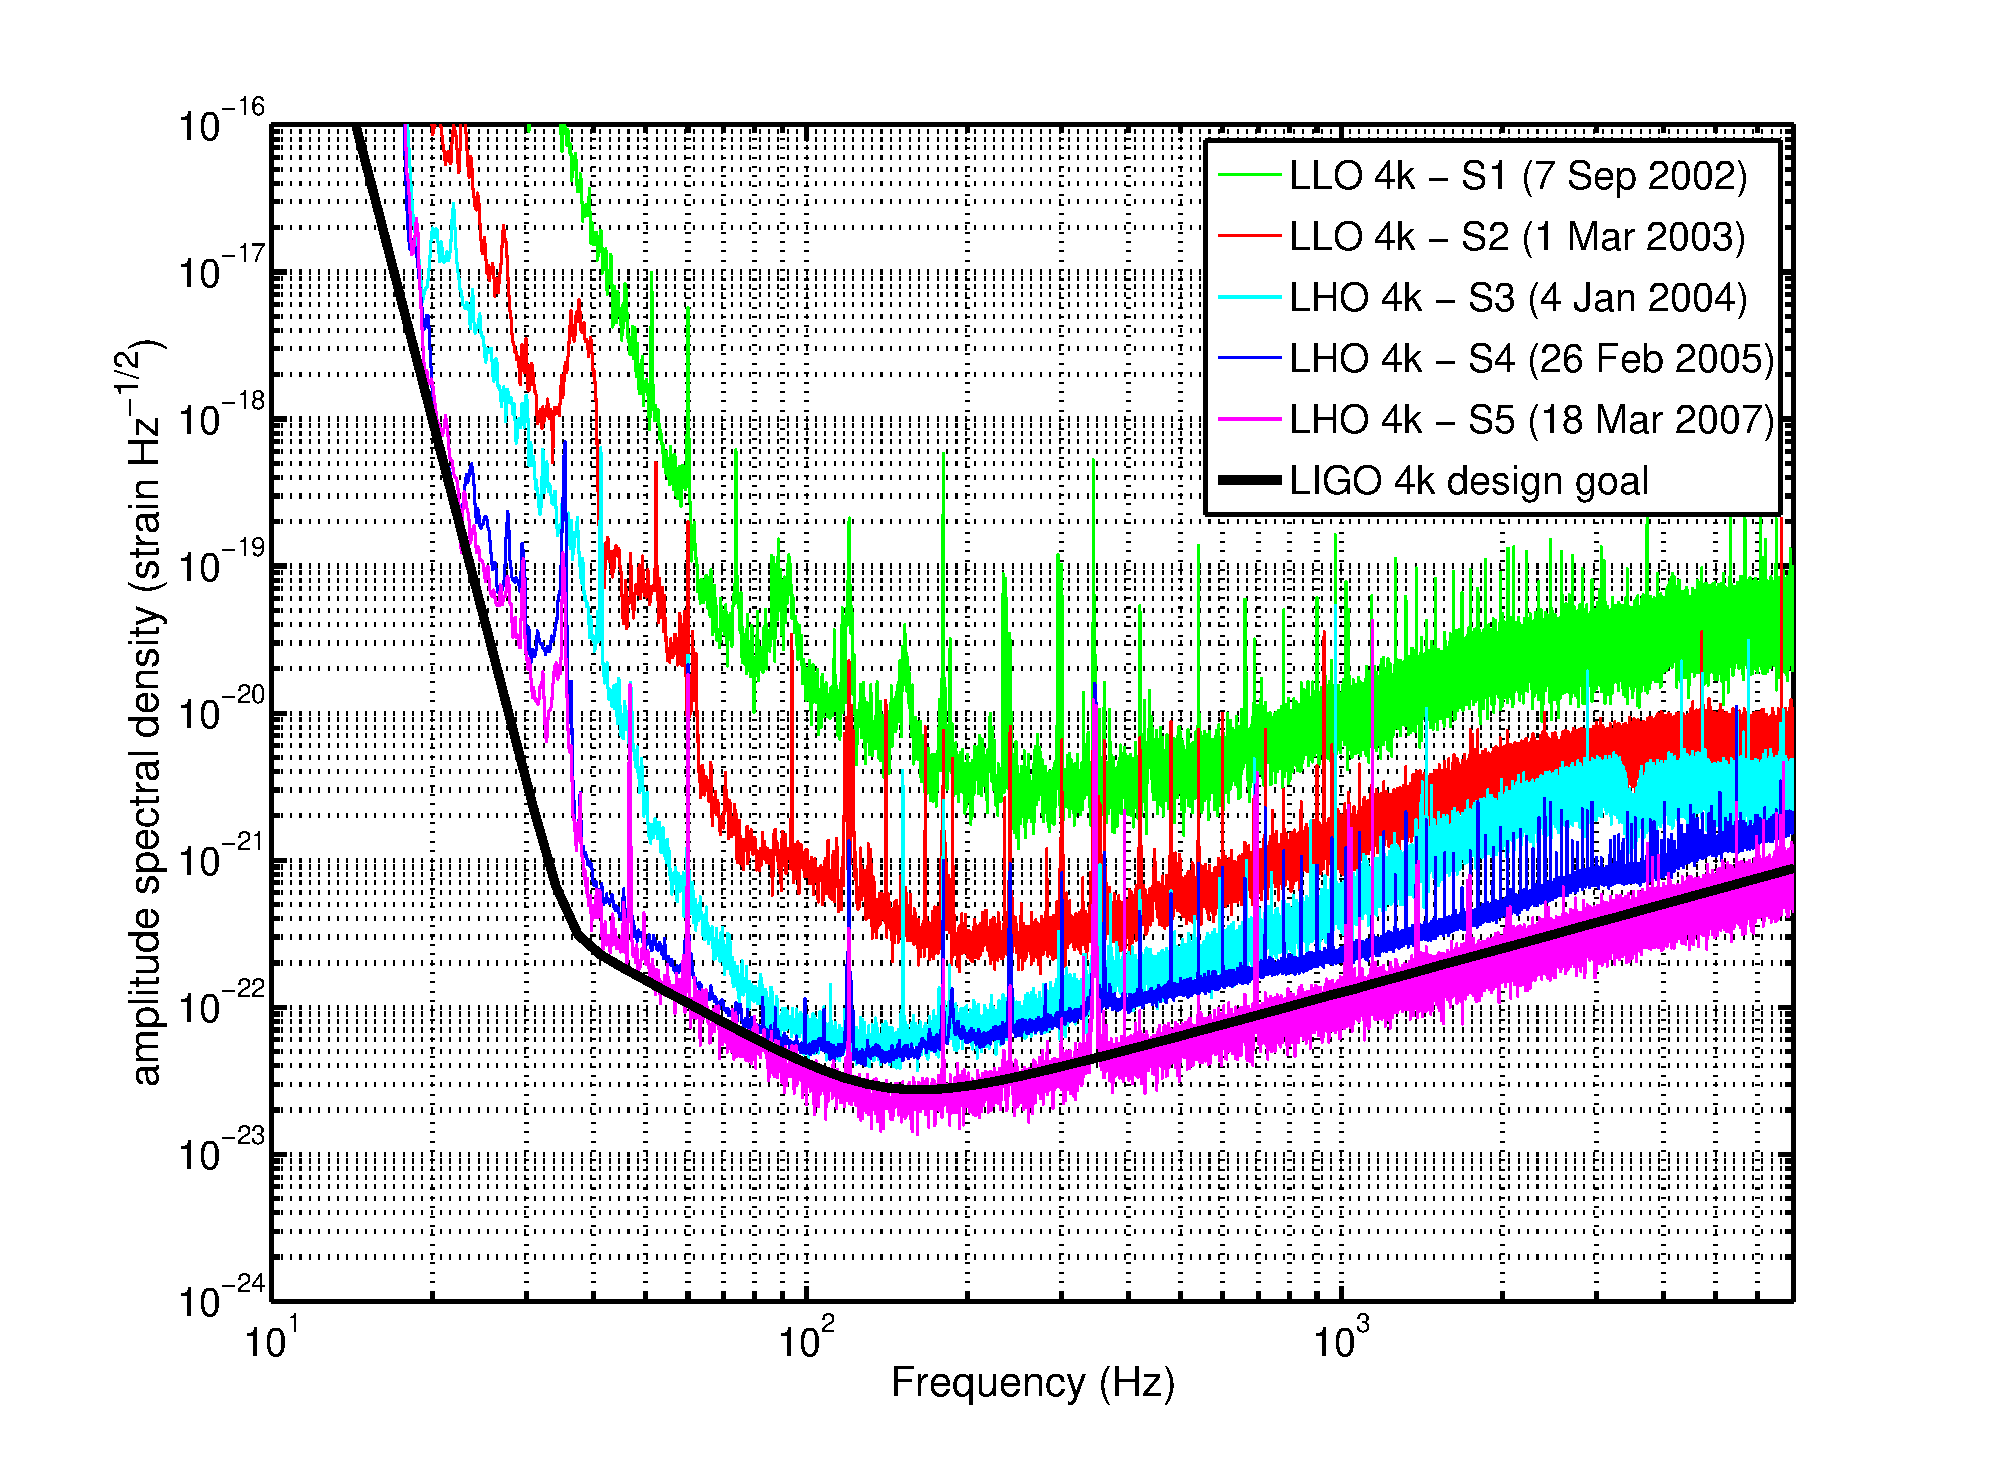
\includegraphics[scale=0.45]{LIGOSrunASDs}}
  \caption{\it The best strain sensitivities from the LIGO science runs S1
through S6 \cite{LIGOcurves}. The S6 curve is 
preliminary and based on h(t) data that has not been completely reviewed
and may be subject to change. Also shown is the LIGO 4~km design sensitivity.}
  \label{figure:LIGOstrains}
\end{figure}}

For the second science run (S2), from 14 February to 14 April 2003, the noise
floor was considerably improved over S1 by several upgrades including:
improving and stabilising the optical levers used to measure the mirror
orientation to reduce the low frequency ($\lesssim$50~Hz) noise; replacing the
coil drivers that are used as actuators to control the position and
orientation of suspended mirrors, to improve the mid-frequency
($\sim$50--200~Hz) noise floor; and increasing the laser power in the
interferometer to reduce shot noise and improve the high frequency
($\gtrsim$200~Hz) sensitivity (see \S{}IIA of \cite{Abbott:2005a} for a more
thorough description of the detector improvements made for S2). These changes
improved the sensitivities by about an order of magnitude across the frequency
band with a best strain, for L1, of $\sim3\times10^{-22}\,{\rm Hz}^{-1/2}$
between 200--300~Hz. The duty factor during S2 was 74\% for H1, 58\% for H2 and
38\% for L1, with a triple coincidence time when all three detectors were in
lock of 22\% of the run. The average inspiral ranges during the run
were approximately 0.9, 0.4 and 0.3\,Mpc for L1, H1 and H2 respectively. This run was also
operated in coincidence with the TAMA~300 DT8 run.

For the the third science run (S3), between 31 October 2003 to 9 January 2004,
the detectors were again improved, with the majority of sensitivity increase in
the mid-frequency range. This run was also operated partially in coincidence
with GEO~600. The best sensitivity, which was for H1, was
$\sim5\times10^{-23}\,{\rm Hz}^{-1/2}$ between 100--200~Hz. The duty factors
were 69\% for H1, 63\% for H2 and only 22\% for L1, with a 16\% triple
coincidence time. L1's poor duty factor was due to large levels of anthropogenic
seismic noise near the site during the day.

The fourth science run (S4), from 22 February to 23 March 2005, saw less drastic
improvements in detector sensitivity across a wide frequency band, but did make
large improvements for frequencies $\lesssim 70$~Hz. Between S3 and S4 a better
seismic isolation system, which actively measured and countered for ground
motion, was installed in L1, greatly reducing the amount of time
it was thrown out of lock. For H1 the laser power was able to be increased to 
its full design power of 10~W \cite{Abbott:2007b}. The duty factors were 80\% for H1,
81\% for H2 and 74\% for L1, with a 56\% triple coincidence time. The most
sensitive detector, H1, had an inspiral range of 7.1\,Mpc.

By mid-to-late 2005 the detectors had equalled their design sensitivities over
most of the frequency band and were also maintaining good stability and high
duty factors. It was decided to perform a long science run with the aim of
collecting one years worth of triple coincident data, with an angle averaged
inspiral range of equal to, or greater than, 10\,Mpc for L1 and H1, and 5\,Mpc
or better for H2. This run, S5, spanned from 4 November 2005 (L1 started
slightly later on 14 November) until 1 October 2007, and the performance of the
detectors during it is summarised in \cite{LIGOS5}. One year of triple
coincidence was achieved on 21 September 2007, with a total triple coincidence
duty factor of 52.5\% for the whole run. The average insprial range over S5
was $\sim15$\,Mpc for H1 and L1, and $\sim8$\,Mpc for H2.

After the end of S5 the LIGO H2 detector and GEO~600 were kept operational
while possible in an evening and weekend mode called Astrowatch. This
observing mode continued until early 2009, after which H2 was decommissioned.
During this time commissioning of some upgrades to the 4~km LIGO detectors took
place for the sixth and final initial LIGO science run (S6) - some of which are
summarised in \cite{Whitcomb:2008}. The aim of these upgrades, called Enhanced 
LIGO \cite{EnhancedLIGO}, was to try and  increase sensitivity by a factor of two. 
Enhanced LIGO involved the direct implementation of technologies and techniques 
designed for the later upgrade to Advanced LIGO (see \S\ref{subsection:aligo}) 
such as, most notably, higher powered lasers, a DC readout
scheme, the addition of output mode cleaners and the movement of some hardware
into the vacuum system. The lasers, supplied by the Albert Einstein Institute
and manufactured by Laser Zentrum Hannover, give a maximum power of $\approx30$~W, 
which is around 3 times the initial LIGO power. The upgrade to higher power required that
several of the optical components needed to be replaced. These upgrades were only
carried out on the 4km H1 and L1 detectors due to the H2 detector being
left in Astrowatch mode during the commissioning period. The upgrades were able 
to produce 1.5-2 times sensitivity increases at frequencies above $\approx 200$~Hz, 
but generally at lower frequencies various sources of noise meant sensitivity 
increases were not possible. S6 took place from July 2009 until 20 October 
2010, at which point decommissioning started for the full upgrade to Advanced LIGO. 
Typically the detectors ran with laser power at $\approx10$~W during the day (at
higher power the detector was less stable and the higher level of anthropogenic 
noise during the day meant that achieving and maintaining lock required lower
power) and $\approx 20$~W at night, leading to inspiral ranges from 
$\approx 10-20$\,Mpc.

\subsubsection{GEO~600}
GEO~600 achieved first lock as a power-recycled Michelson (with no signal
recycling) in late 2001. Commissioning over the following year, detailed in
\cite{Hewitson:2003}, included increases in the laser power, installation of
monolithic suspensions for the end test masses (although not for the beam
splitter and inboard mirrors), rearrangement of the optical bench to reduce
scattered light and implementation of an automatic alignment system. For the S1
run, carried out in coincidence with LIGO (and, in part, TAMA~300), the detector
was kept in this configuration (see \cite{Abbott:2004a} for the status of the
detector during S1). It had a very high duty factor of $\sim98\%$, although
it's strain sensitivity was $\sim2$ orders of magnitude lower than the LIGO
instruments. The auto-alignment system in GEO~600 has since meant that it has
been able to operate for long periods without manual intervention to regain
lock, as has been the case for initial LIGO.

% GEO S1 through S5 typical strain sensitivities
\epubtkImage{}{%
\begin{figure}[hptb]
  \centerline{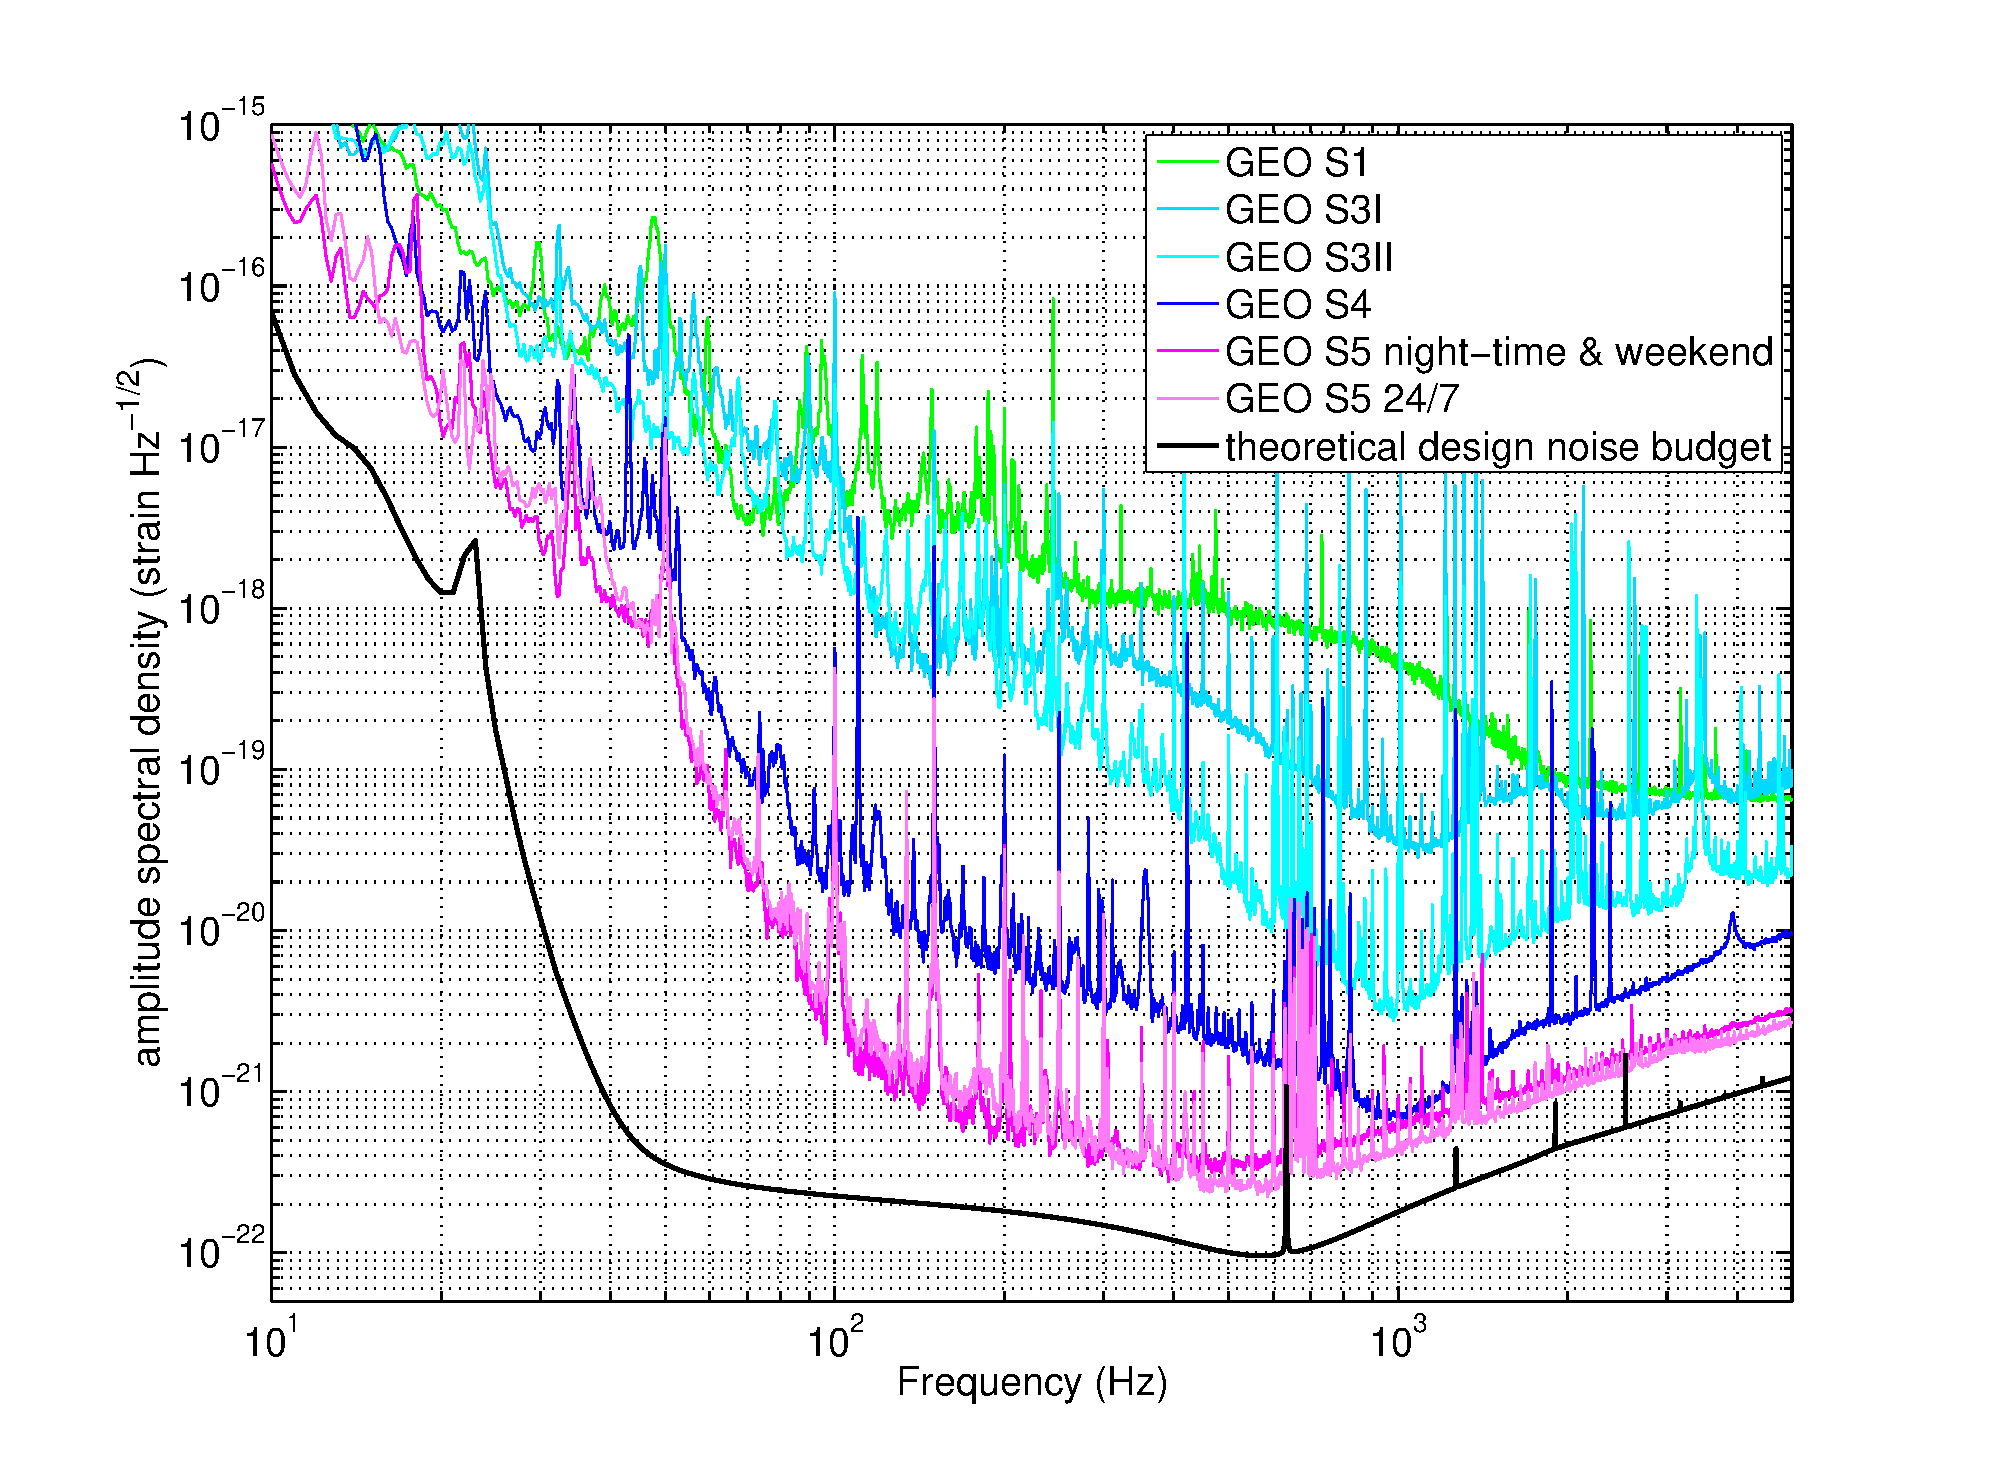
\includegraphics[scale=0.45]{GEOSrunASDs}}
  \caption{\it The typical strain sensitivities from the GEO~600 science runs S1
through S5 \cite{GEOcurves}. Also shown is the theoretical noise budget for
the detector when tuned to 550~Hz -- the operating position for the S5 run.}
  \label{figure:GEOstrains}
\end{figure}}

Following S1 the signal recycling mirror was installed and in late 2003 the
first lock of the fully dual-recycled system was achieved (see
\cite{Smith:2004, Willke:2004, Grote:2005} for information on the commissioning
of GEO~600 as a dual-recycled detector). Other upgrades included the
installation of the final mirrors, suspended as triple pendulums, and with
monolithic final stages. Once installed it was found that there was a radius of
curvature mismatch with one of the mirrors, which had to be compensated for by
carefully heating the mirror. Due to this commissioning effort GEO~600 did not
participate in the S2 run. Very soon after the implementation of dual-recycling
GEO~600 took part in the S3 run. This occurred over two time intervals
from 5--11 November 2003, dubbed S3I, and from 30 December 2003 to 13 January
2004, dubbed S3II. During S3I GEO~600 operated with the signal-recycling
cavity tuned to $\sim 1.3$\,kHz, and had a $\sim$95\% duty factor, but was then
taken off-line for more commissioning work. In the period between S3I and II
various sources of noise and lock loss were diagnosed and mitigated, including
noise from a servo in the signal recycling cavity and electronic noise on a
photo-diode \cite{Smith:2004}. This lead to improved sensitivity by up to an
order of magnitude at some frequencies (see Fig.~\ref{figure:GEOstrains}). For
S3II the signal recycling cavity was tuned to 1\,kHz and, due to the upgrades,
had an increased duty factor of $\sim$99\%.

GEO~600 operated during the whole of S4 (22 February to 24 March 2004), in
coincidence with LIGO, with a $\sim$97\% duty factor. It used the same optical
configuration as S3, but had sensitivity improvements from a few times to up
to over an order of magnitude over the S3 values \cite{Hild:2006a}.

The main changes to the detector after S4 were to shift the resonance condition
of the signal recycling cavity to a lower frequency, 350~Hz, allowing better
sensitivity in the few hundred Hz regime, and increasing the circulating laser
power, with an input power of 10\,W. The pre-S5 peak sensitivity was
$\sim4\times10^{-22}\,{\rm Hz}^{-1/2}$ at around 400~Hz, with an inspiral
range of 0.6\,Mpc \cite{Hild:2006b}. GEO~600 did not join S5 at the
start of the LIGO run, but from 21 January 2006 was in a night and weekend data
taking mode whilst noise hunting studies and commissioning were conducted. For
S5 the signal recycling cavity was re-tuned up to 550~Hz. It went into full time
data taking from 1 May to 16 October 2006, with an instrumental duty factor of
94\%. The average peak sensitivity during S5 was better than
$3\times10^{-22}\,{\rm Hz}^{-1/2}$ (see \cite{Willke:2007} for a summary of
GEO~600 during S5). After this it was deemed more valuable for GEO~600 to
continue more noise hunting and commissioning work, to give as good a
sensitivity as possible for when the LIGO detectors went offline for upgrading.
It did however continue operating in night and weekend mode. 

GEO~600  continued operating in Astrowatch mode between November 2007 and July 
2009 after which upgrades began. The plans for the GEO~600 detector are to 
continue to use it as a test-bed for more novel interferometric techniques whilst 
focusing on increasing in sensitivity at higher frequencies (greater than a 
few hundred Hz). This project is called
GEO-HF \cite{Willke:2006}. The upgrading towards GEO-HF has been taking
place since summer 2009 \cite{Grote:2010}. The main upgrades started during 2009 
were to change the read-out scheme from an RF read-out to a DC read-out system 
\cite{Hild:2008}, 
install an output mode cleaner, place the read-out system in vacuum, injecting 
squeezed light \cite{Vahlbruch:2008, Chelkowski:2007} into the output port, and 
finally increasing the input laser power to 35~W. Running the interferometer
with squeezed light will be the first demonstration of a full-scale gravitational
wave detector operating beyond the standard quantum limit. GEO-HF participated in 
S6 in an overnight and weekend mode, alongside a commissioning schedule, and is 
continuing in this mode following the end of S6.

\subsubsection{Virgo}
In summer 2002 Virgo completed the commissioning of the central area
interferometer, consisting of a power-recycled Michelson interferometer, but
without the 3\,km Fabry-Perot arm cavities. Over the next couple of years
various steps were made towards commissioning the full size interferometer. In
early 2004 first lock with the 3~km arms was achieved, but without
power-recycling, and by the end of 2004 lock with power recycling was achieved.
During summer 2005 the commissioning runs provided order of magnitude
sensitivity improvements, with a peak sensitivity of $6\times10^{-22}\,{\rm
Hz}^{-1/2}$ at 300~Hz, and an inspiral range of over 1\,Mpc. In late 2005
several major upgrades brought Virgo to its final configuration. See
\cite{Acernese:2004, Acernese:2005, Acernese:2006, Acernese:2007} for more
detailed information on the commissioning of the detector.

Virgo joined coincident observations with the LIGO and GEO~600 S5 run with
10 weekend science runs (WSRs) starting in late 2006 until March 2007. Over this
time improvements were made mainly in the mid-to-low frequency regime ($\lesssim
300$~Hz). Full-time data taking, under the title of Virgo Science run 1 (VSR1),
began on 18 May 2007 and ended with the end of S5 on 1 October 2007. During VSR1
the science mode duty factor was 81\% and by the end of the run maximum binary
neutron star inspiral range was frequently up to about 4.5\,Mpc. The best
sensitivity curves for WSR1, WSR10 and VSR1 can be seen in
Fig~\ref{figure:Virgostrains}.

% Virgo typical strain sensitivities
\epubtkImage{}{%
\begin{figure}[hptb]
  \centerline{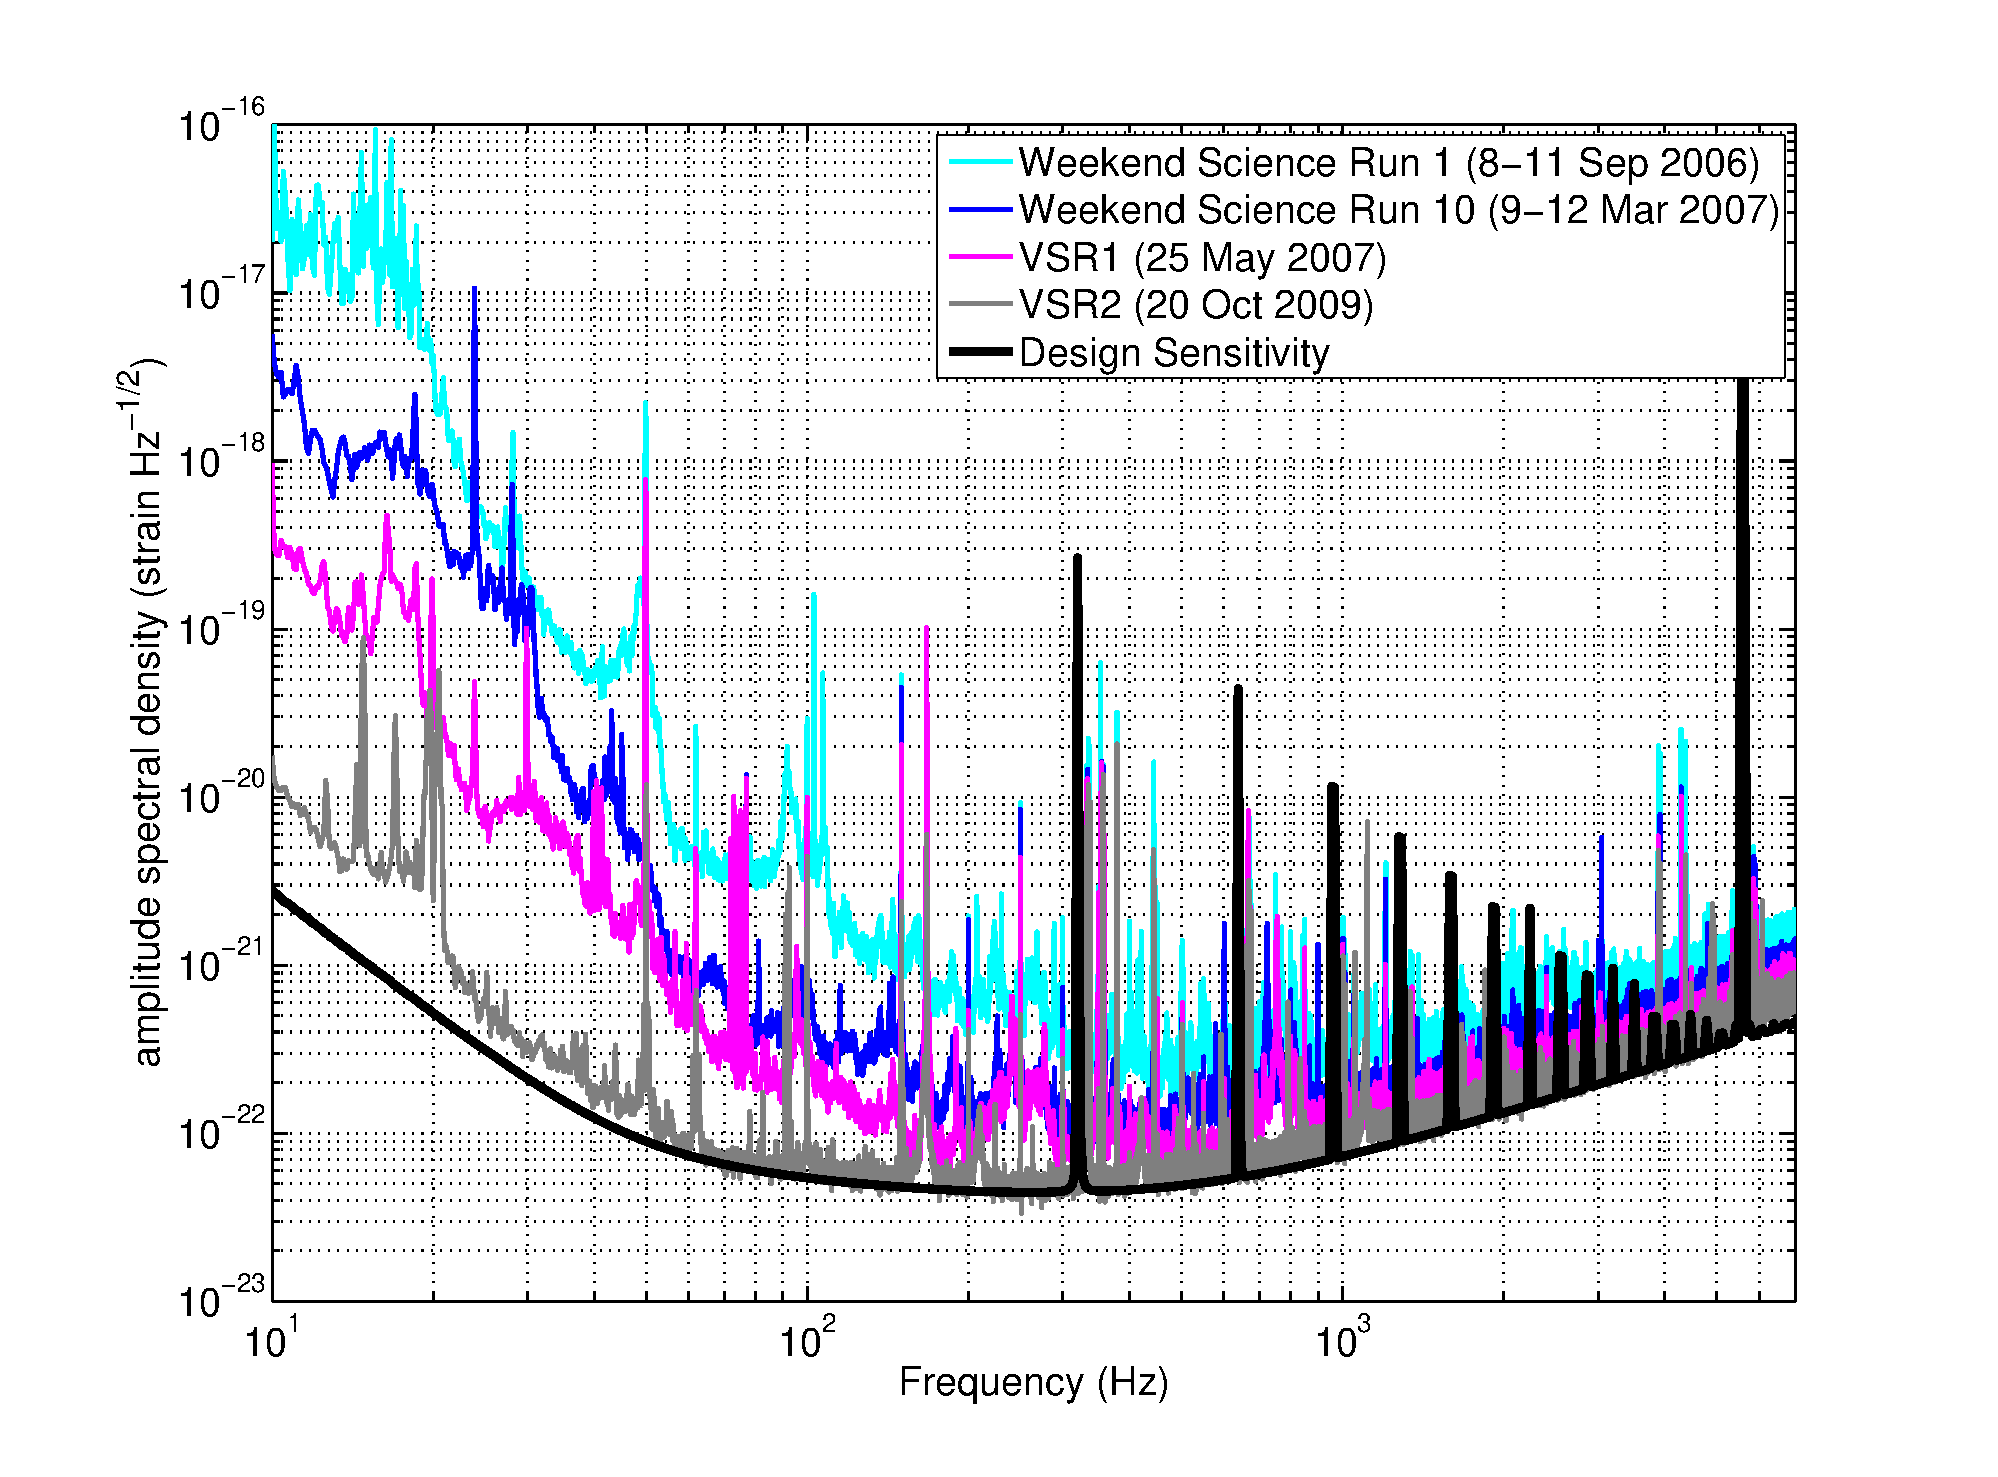
\includegraphics[scale=0.45]{VirgoSrunASDs}}
  \caption{\it The best strain sensitivities from the Virgo weekend and full
time science runs WSR1, WSR10, VSR1 and VSR2 \cite{Virgocurves, VSR2paper}.}
  \label{figure:Virgostrains}
\end{figure}}

At the same time as commissioning for Enhanced LIGO was taking place there
was also a similar effort to upgrade the Virgo detector, called Virgo+.
The main upgrade was to the lasers to increase their power from 10 to 25~W at
the input mode cleaner, with upgrades also to the thermal compensation system
on the mirrors, the control electronics, mode cleaners and injection optics
\cite{Acernese:2008b, AdVwhitepaper}. Virgo+ started taking data with
Enhanced LIGO for Virgo Science Run 2 (VSR2) and sensitivities of Virgo+ close to
the initial Virgo design sensitivity were reached. VSR2 finished on 8 January 2010
to allow for further commissioning and noise hunting. This has since been followed
by VSR3, which began on 11 August 2010 and is expected to finish at the start of
July 2011. A further Virgo+ run, VSR4, is expected to follow this and last for
about 6 months from mid-2011. Following this the upgrades to Advanced Virgo will begin.

\subsection{Astrophysics Results}\label{subsection:results}
Prior to the advent of the large scale interferometric detectors there had
been some limited effort to produce astrophysical results with the prototype
interferometers. The Caltech 40~m detector was used to search for, and set an
upper limit on, the gravitational wave emission from pulsar PSR\,J1939+2134
\cite{Hereld:1984}, and on the rate of neutron star binary
inspirals in our galaxy, using coincident observations with the University of
Glasgow prototype \cite{Smith:1988} and, more recently, on its own
\cite{Allen:1999}. Coincident observations using the prototype detectors at the
University of Glasgow and Max Planck Institute for Quantum Optics, in Garching,
Germany, were used to set an upper limit on the strain of gravitational wave
bursts \cite{Nicholson:1996}. The Garching detector was used to search for
periodic signals from pulsars, and in particular set a limit on a potential
source in SN1987A \cite{Niebauer:1993}. However since the start of science data
taking for the large scale detectors there has been a rapid rise in the number,
and scope, of science result papers being published. With the vastly improved
sensitivities pushing upper limits on source populations and strengths towards
astrophysically interesting areas.

The recent analysis efforts have generally been split into four broad areas
depending on the expected signal type: unmodelled transients or bursts e.g. supernova;
modelled transients e.g. inspirals and ring-downs (or more specifically compact
binary coalescences, CBC); continuous sources;
stochastic sources. Within each area a variety of different sources could
exist and a variety of analysis techniques have been developed to search for
them. Some electromagnetic sources, such as radio pulsars and $\gamma$-ray
bursts, are also used to enhance searches. A good review of the data analysis 
methods used in current searches, and the astrophysical consequences of some of
the results described below, can be found in \cite{Sathyaprakash:2009}.

Here we will briefly summarise the main astrophysics results from the science 
runs. We will mainly focus on those produced by the LIGO Scientific
Collaboration \cite{LSCweb} detectors LIGO and GEO~600 from S1 to the S5 run. 
At the time of writing not all of the data from the S6 run had been
fully analysed, with more results expected over the next year. Reviews of some
early S5, and previous science run, results can also be found in
\cite{Papa:2008, Fairhurst:2009}. In none of the searches so far has convincing
evidence for a gravitational wave signal been seen.

\subsubsection{Unmodelled bursts}\label{subsubsection:unmodelled}
Searches for unmodelled bursts, e.g.~from supernova core-collapse, are based on
looking for short duration periods of excess power in the detectors. Transients
are common features in the data, so to veto these events from true
gravitational wave signals they must be coincident in time, and to some extent
amplitude and waveform, between multiple detectors. Various methods to assess
instrumental excess power, and inter-detector correlations, are used, some
examples of which can be found here \cite{Klimenko:2004, Anderson:2001,
Searle:2008, McNabb:2004, Cadonati:2004, Chatterji:2004, Chatterji:2006}. These
algorithms will produce {\it triggers}, which are periods of excess power that
cross a predetermined signal-to-noise ratio threshold (determined by tuning the
algorithms on a section of {\it playground} data, so that the output produces a
desired false alarm rate). The number of triggers are then compared to a
background rate. Real signals cannot be turned off, and detectors cannot be 
shielded from them, so the background rate has to be approximated by time shifting one
detector's data stream with respect the the others. Time shifts should only
leave triggers due to random coincidences in detector noise and there should
be no contribution from real signals. Once a background is calculated the
statistical significance of the foreground rate can be compared to it. To assess
the sensitivity of these searches, hardware (the interferometer mirrors are
physically moved via the control system) and software signals are injected into
the data stream at various strengths and the efficiency of the algorithms at
detecting them is measured. A good description of some of these techniques can be
found in \cite{Abbott:2004b} and \cite{Abbott:2006a}.

Data from the LIGO S1 run was searched for gravitational wave bursts of between
4 to 100\,ms, and within the frequency band 150 to 3000~Hz \cite{Abbott:2004b}.
Triple coincident data from all three detectors was used for the analysis. No
plausible candidate event was found, but a 90\% confidence upper limit on the
event rate of 1.6 events per day was set. The search was typically
sensitive, at a $\gtrsim50\%$ detection efficiency, to bursts with amplitudes of
$h_{\rm rss}\sim10^{-19}-10^{-17}\,{\rm Hz}^{-1/2}$ (defined in terms of $h_{\rm
rss} \equiv \sqrt{\int|h|^2{\rm d}t}$, which is the root-sum-squared strain amplitude
spectral density). Due, in part, to its lower sensitivity GEO~600 data was
not used in this analysis. The S2 data's improved sensitivity, and advances in
the analysis techniques, allowed a sensitivity to signals (in the frequency
range 100--1100~Hz) in the amplitude range $h_{\rm
rss}\sim10^{-20}-10^{-19}\,{\rm Hz}^{-1/2}$ \cite{Abbott:2005a}. Interpreting
the best sensitivities astrophysically gave order of magnitude estimates on
the visible range of $\sim100$\,pc for a class of theoretical supernova
waveforms, and 1\,Mpc for the merger of $50\,{\rm M}_{\odot}$ black holes. Again
no signal was seen, but a 90\% upper limit of 0.26 events per day was set for
strong bursts. In the frequency range 700--2000~Hz TAMA~300 data was also used
in the search giving amplitudes sensitivities of $h_{\rm
rss}\sim1-3\times10^{-19}\,{\rm Hz}^{-1/2}$ and decreasing the rate upper limit
to 0.12 events per day \cite{Abbott:2005c}.

The S3 run produced two searches for burst sources. One used the 8 days of
triple coincidence data from the three LIGO detectors to search for sub-second
bursts in the frequency range 100--1100~Hz \cite{Abbott:2006a}. The search was
sensitive to signals with amplitudes over $h_{\rm rss}\sim1\times10^{-20}\,{\rm
Hz}^{-1/2}$, but did not include an astrophysical interpretation of the limit or
event rate upper limit. This run included coincident operation with the Italian
AURIGA bar detector and this data has been analysed \cite{Baggio:2008}. This
search looked for short bursts of less than 20~ms within the 850--950~Hz band
(around the bar's sensitive resonant frequency). This had comparable sensitivity
to the LIGO-only S2 search and produced a 90\% confidence rate upper limit of
0.52 events/day.

For S4 15.5 days of LIGO data were searched for sub-second bursts
in the frequency range 64--1600~Hz \cite{Abbott:2007b}. This was sensitive to
signals with $h_{\rm rss}\lesssim10^{-20}$ and set a 90\% confidence rate
upper limit of 0.15 per day. The search results are also cast as astrophysical
limits on source ranges and energetics. These show that there would be a 50\%
detection efficiency to signals of sine-Gaussian nature (at the most sensitive 
frequency of 153~Hz and quality factor $Q=8.9$) at a distance of 10~kpc for an
energy of $10^{-7}$\,M$_{\odot}c^2$, and would be sensitive to signals out to
the Virgo cluster ($\sim16$\,Mpc) for an energy release of
$0.25$\,M$_{\odot}c^2$. See \cite{Abbott:2007b} for a comparison of previous
burst searches. There was also a burst search combining S4 GEO~600 and LIGO data
for the first time. This searched data between 768--2048~Hz where the
sensitivities were most comparable and used 257 hours of quadruple coincidence
between the detectors and saw no gravitational wave events \cite{Abbott:2008b}.

For the analysis on the first year of S5 data the frequency range for the
all-sky burst search was split -- a low frequency search covered the most
sensitive region between 60--2000\,Hz \cite{Abbott:2009h}, and a high frequency
search covering 1--6\,kHz (this being the first time an
untriggered burst search looked at frequencies above 3\,kHz)
\cite{Abbott:2009i}. The high frequency search
set a 90\% upper limit on the rate of 5.4 events per year for strong events. The
low frequency search analysed more data than the high frequency and set an
event rate limit of 3.6 events per year. The second year of S5 LIGO data was
analysed with GEO~600 and Virgo VSR1 data \cite{Abadie:2010d} to search for 
bursts over the whole 50--6000~Hz band. Combining this with the earlier S5 
searches gave $h_{\rm rss}$ upper limits for a variety of simulated waveforms 
of $6\times10^{-22}\,{\rm Hz}^{-1/2}$ to $2\times10^{-20}\,{\rm Hz}^{-1/2}$, and a
90\% confidence event rate for signals between 64--2048~Hz of less than two 
per year.

\subsubsection{Modelled bursts - compact binary coalescence}\label{sec:cbc}
Modelled bursts generally mean the inspiral and coalescence stage of binaries
consisting of compact objects e.g. neutron stars and black holes. The signals
are generally well approximated by post-Newtonian expansions of the Einstein
equation, which give the amplitude and phase evolution of the orbit. More recently signal
models have started to include numerical relativity simulations of the
merger stage \cite{Aylott:2009}. As mentioned in \S\ref{section:construction} 
the best estimate of the number of signals observable with initial LIGO at design sensitivity 
(i.e.~during S5) would be 0.02 per year (based on an event rate of 
$1\times10^{-6}$ per year per MWEG). 

The majority of inspiral searches make use of matched filtering in which a
template bank of signal models is built \cite{Owen:1996, Owen:1999}, with a
maximum mismatch between templates that is generally of order $\sim10\%$. These
templates are then cross-correlated with the data and statistically significant
{\it triggers} (i.e.\ times when the template and data are highly correlated)
from this are looked for. Triggers must be coincident between detectors and the
significance of any trigger is judged against a background calculated in the
same way as described in \S\ref{subsubsection:unmodelled}. See
\cite{Abbott:2005b} for a good description of the search method.

The first search for an inspiral signal with data from the LIGO S1 run looked
for compact object coalescences with component masses between 1--3\,M$_{\odot}$
and was sensitive to such sources within the Milky Way and Magellanic Clouds
\cite{Abbott:2004c}. It gave a 90\% confidence level upper limit on the rate of
170 per year per MWEG.

For the S2 LIGO analysis the search was split into 3 areas covering neutron star
binaries, black hole binaries and primordial black hole binaries in the galactic
halo. The neutron star binary search \cite{Abbott:2005b} used 15 days of data
with coincidence between either H1 and L1 or H2 and L1. It had a range of
$\sim1.5$\,Mpc, which spanned the Local Group of galaxies, and gave a 90\% event
rate upper limit on systems with component masses of 1--3\,M$_{\odot}$ of 47 per
year per MWEG. The binary black hole search looked for systems with component
masses in the 3--20\,M$_{\odot}$ range using the same data set as the binary
neutron star search \cite{Abbott:2006a}. This search had a 90\% detection
efficiency for sources out to 1\,Mpc and set a 90\% rate upper limit of 38 per
year per MWEG. The third search looked for low mass (0.2--1\,M$_{\odot}$)
primordial black hole binaries in a 50\,kpc radius halo surrounding the Milky
Way \cite{Abbott:2005e}. This placed a 90\% confidence rate upper limit of 63
events per year per Milky Way halo. The S2 search was performed in coincidence
with the TAMA~300 DT8 period and an inspiral search for neutron star binaries was
performed on data when TAMA~300 and at least one of the LIGO sites was
operational. This gave a total of 584 hours of data for the analysis, which set
a 90\% rate upper limit of 49 per year per MWEG, although this search was only
sensitive to sources within the majority of the Milky Way \cite{Abbott:2006b}.

The search for neutron star-black hole binaries in S3 LIGO data used techniques
designed specifically for systems with spinning components. It searched for
systems with component masses in the range 1--20\,M$_{\odot}$ and analysed 167
hours of triple coincident data and 548 hours of H1-H2 data to set the upper
limits \cite{Abbott:2008d}. For a typical system with neutron star and black
hole mass distributions centred on 1.35\,M$_{\odot}$ and 5\,M$_{\odot}$ (from
the population statistics discussed in \cite{Abbott:2008a}) this search produced
a 90\% confidence rate upper limit of 15.9 per year per $L_{10}$.

The search for a wide range of binary systems with components consisting of
primordial black holes, neutron stars, and black holes with masses in
the ranges given above was conducted on the combined S3 and S4 data
\cite{Abbott:2008a}. 788 hours of S3 data and 576 hours of S4 data were used
and no plausible gravitational wave candidate was found. The highest mass range
for the binary black hole search was set at 40\Msun for S3 and 80\Msun for S4.
At peak in the mass distribution of these sources 90\% confidence rate upper
limits were set at 4.9 per year per $L_{10}$ for primordial black holes, 1.2 per
year per $L_{10}$ for binary neutron stars, and 0.5 per year per $L_{10}$ for
binary black holes. S4 data has also been used to search for ring-downs from
perturbed black holes, for example following binary black hole coalescence
\cite{Abbott:2009g}. The search was sensitive to ring-downs from
10--500\,M$_{\odot}$ black holes out to a maximum range of 300\,Mpc, and
produced a best 90\% confidence upper limit on the rate of ring-downs to be
$1.6\times10^{-3}$ per year per $L_{10}$ for the mass range
85--390\,M$_{\odot}$.

One other kind of modelled burst search is that looking for gravitational waves
produced by cusps in cosmic (super)strings. Just over two weeks of LIGO S4 data
were used to search for such signals \cite{Abbott:2009j}. This was used to
constrain the rate and parameter space (string tension, reconnection
probability, and loop sizes), but was not able to beat limits set by Big Bang
nucleosynthesis.

Data from the first \cite{Abbott:2009e} and second year of S5 (prior to Virgo
joining with VSR1) \cite{Abbott:2009f} have been searched for low-mass binary
coalescences with total masses in the range 2--35\,M$_{\odot}$. The second
year search results have produced the more stringent upper limits with 90\%
confidence rates for binary neutron star, binary black hole and
neutron star--black hole systems respectively of $1.4\times10^{-2}$,
$7.3\times10^{-4}$ and $3.6\times10^{-3}$ per year per $L_{10}$. Five months of
overlapping S5 and VSR1 data were also searched for the same range of signals 
\cite{Abadie:2010f} giving 90\% confidence upper rates of $8.7\times10^{-3}$ per year per $L_{10}$, 
$2.2\times10^{-3}$ per year per $L_{10}$, and $4.4\times10^{-4}$ per year per $L_{10}$.

\subsubsection{Externally triggered burst searches}
Many gravitational wave burst sources will be associated with 
electromagnetic (or neutrino) counterparts, for example short $\gamma$-ray 
bursts (GRBs) are potentially caused by black hole and neutron star coalescences.
Joint observation of a source as both a gravitational wave and electromagnetic
event also greatly increases the confidence in a detection. Therefore many 
searches have been performed to look for bursts coincident (temporally and 
spatially) with external electromagnetic triggers, such as GRBs observed by 
Swift for example. These searches have
used both excess power and modelled matched filter methods to look for signals.

During S2 a particularly bright $\gamma$-ray burst event (GRB~030329) occurred 
and was specifically targeted using data from H1 and H2. The search looked for a 
signals with duration less than $\sim 150$~ms and in the frequency range 80--2048~Hz
\cite{Abbott:2005d}. This produced a best strain upper limit for an unpolarised
signal around the most sensitive region at  $\sim250$~Hz of $h_{\rm
rss}=6\times10^{-21}\,{\rm Hz}^{-1/2}$.

For S4 there were two burst searches targeting specific sources. The first target was
the hyperflare from the Soft $\gamma$-ray Repeater SGR 1806$-$20 (SGRs are
thought to be ``magnetars'', neutron stars with extremely large magnetic fields
of order $10^{15}$ Gauss) on the 27$^{\rm th}$ December 2004 \cite{Hurley:2005}
(this actually occurred before S4 in a period when only the H1 detector was
operating). The search looked for signals at frequencies corresponding to short
duration quasi-periodic oscillations (QPOs) observed in the X-ray light curve
following the flare \cite{Abbott:2007c}. The most sensitive 90\% upper limit was
for the 92.5~Hz QPO at $h_{\rm rss} = 4.5\times10^{-22}$\,Hz$^{-1/2}$, which
corresponds to an energy emission limit of $4.3\times10^{-8}$M$_{\odot}c^2$ (of
the same order as the total electromagnetic emission assuming isotropy). The
other search used LIGO data from S2, S3 and S4 to look for signals associated
with 39 short duration $\gamma$-ray bursts (GRBs) that occurred in coincidence
with these runs \cite{Abbott:2008c}. The GRB triggers were provided by IPN,
Konus-Wind, HETE-2, INTEGRAL and Swift as distributed by the GRB Coordinate
Network \cite{GCN}. The search looked in a 180 second window around the burst
peak time (120 seconds before and 60 seconds after) and for each burst there were
at least two detectors contributing data. No signal coincident with a GRB was
observed and the sensitivities were not enough to give any meaningful
astrophysical constraints, although simulations suggest that for S4, as in the general burst search,
it would have been sensitive to sine-Gaussian signals out to tens of Mpc for an
energy release of order a solar mass.

The first search of Virgo data in coincidence with a GRB was performed on data
from a commissioning run in September 2005. The long duration GRB~050915a was observed
by Swift on 15 September 2005 and Virgo data was used to search for an 
unmodelled burst in a window of 180 seconds around (120 s before and 60 s after)
the GRB peak time \cite{Acernese:2008a}. The search produced a strain upper
limit of order $10^{-20}$ in the frequency range 200--1500 Hz, but was mainly
used as a test-bed for setting up the methodology for future searches, including
coincidence analysis with LIGO.

Data from the S5 run has been used to search for signals associated with even more
$\gamma$-ray bursts. One search looked specifically for emission from
GRB~070201 \cite{Golenetskii:2007a, Golenetskii:2007b}, which
was potentially associated with originating in the nearby Andromeda galaxy
(M31). The data around the time of this burst was used to look for an
unmodelled burst and an inspiral signal as might be expected from a short GRB.
The analysis saw no gravitational wave event associated with the GRB, but
ruled out the event being a binary neutron star inspiral located in M31 with a
99\% confidence \cite{Abbott:2008g}. Again assuming a binary neutron star
inspiral, but located outside M31, the analysis set a 90\% confidence
limit that the source must be at a distance greater than 3.5\,Mpc. 
Assuming a signal again located in M31 the unmodelled burst search set an upper 
limit on the energy
emitted via gravitational waves of $4.4\times10^{-4}\,M_{\odot}$c$^2$, which was 
well within the allowable range for this being an SGR hyper-flare in M31. Searches for 137
GRBs (both short and long GRBs) that were observed, mainly with the Swift
satellite, during S5 and VSR1 have been performed again using unmodelled 
burst methods \cite{Abbott:2009d} and for (22 short bursts) inspiral 
signals \cite{Abadie:2010b}. No evidence for a gravitational wave signal 
coincident with these events was seen.
The unmodelled burst observations were used to set lower limits on the 
distance to each GRB, with typical limits, assuming isotropic emission, 
at $D\sim15\,{\rm Mpc}(E^{\rm iso}_{\rm GW}/0.01\,M_{\odot}c^2)^{1/2}$. The 
inspiral search, which was sensitive to CBCs with total system masses between
$2\,M_{\odot}$ and $40\,M_{\odot}$, was able to exclude with 90\% confidence 
any bursts being neutron star-black hole mergers within 6.7~Mpc, although the
peak distance distribution of GRBs is well beyond this.

Another search has been to look for gravitational waves associated with flares
from known SGRs and anomalous X-ray pulsars (AXPs), both of which are thought to
be {\it magnetars}. During the first year of 
S5 there were 191 (including the
December 2004 SGR 1806$-$20 event) observed flares from SGRs 1806$-$20 and
1900+14 for which at least one LIGO detector was online \cite{Abbott:2008h}, and 1279 flare events if
extending that to six known galactic magnetars and including all S5 and post-S5 Astrowatch 
data including Virgo and GEO~600 \cite{Abadie:2010c}. The
data around each event was searched for ring-down signals in the
frequency range 1--3\,kHz and with decay times 100--400 ms as might be expected
from $f$-mode oscillations in a neutron star. It was also searched for unmodelled
bursts in the 100--1000 Hz range. No gravitational bursts were seen from any of
the events. For the earlier search \cite{Abbott:2008h} the lowest 90\% upper 
limit on the gravitational wave energy from
the ring-down search was $E_{\rm GW}^{90\%} = 2.4\times10^{48}$ erg for an SGR
1806$-$20 burst on 24 August 2006. The lowest 90\% upper limit on the unmodelled
search was $E_{\rm GW}^{90\%} = 2.9\times10^{45}$ erg for an SGR 1806$-$20
burst on 21 July 2006. The smallest limits on the ratio of energy emitted via
gravitational waves to that emitted in the electromagnetic spectrum were of
order 10--100, which are into a theoretically allowed range. The latter search
\cite{Abadie:2010c} gave the lowest gravitational wave emission energy upper 
limits for white noise bursts in the detector sensitive band, 
and for $f$-mode ring-downs (at 1090 Hz), of $3.0\times10^{44}$~erg and $1.4\times10^{47}$~erg 
respectively, assuming a distance of 1~kpc. The $f$-mode energy limits approach the
range seen emitted electromagnetically during giant flares.
One of these flares, on 29 March 2006, was actually a ``storm'' of many flares 
from SGR\,1900+14. For this event a more sensitive search has been performed by stacking data
around the time of each flare \cite{Abbott:2009c}. Waveform dependent upper
limits of the gravitational wave energy emitted were set between
$2\times10^{45}$\,erg and $6\times10^{50}$\,erg, which are an order of magnitude
lower than the previous upper limit for this storm (included in the search 
of \cite{Abbott:2008h}) and overlap with the range of
electromagnetic energies emitted in SGR giant flares. 

Another possible source of gravitational waves associated with an  
electromagnetically observed phenomenon are pulsar glitches. During these it is
possible that various gravitational wave emitting vibrational modes of the
pulsar may be excited. A search has been performed for fundamental modes ($f$-modes) 
in S5 data following a glitch observed in the timing of the Vela pulsar 
in August 2006  \cite{Abadie:2010a}. Over the search frequency range of 
1--3~kHz this provided upper limits on the peak strain of $0.6-1.4\times10^{-20}$
depending on the spherical harmonic that was excited.

Already efforts are under way to invert this process of searching gravitational 
wave data for external triggers, and instead supplying gravitational wave burst 
triggers for electromagnetic follow-up. This is being investigated across the
range of the electromagnetic spectrum from radio \cite{Predoi:2010}, through
optical (e.g. \cite{Kanner:2008, Coward:2010}) and X-ray/$\gamma$-ray, and even 
looking for coincidence with neutrino detectors \cite{Aso:2008, Pradier:2010, 
Chassande:2010}. Having so-called {\it multi-messenger} observations can have a
large impact on the amount of astrophysical information that can be learnt about an 
event \cite{Phinney:2009}.

\subsubsection{Continuous sources}
Searches for continuous waves focus on rapidly spinning neutron stars as
sources. There are fully targeted searches, which look for gravitational waves
from known radio pulsars in which the position and spin evolution of the objects
are precisely known. There are semi-targeted searches which look at potential
sources in which some, but not all, the source signal parameters are known, for
example neutron stars in X-ray binary systems, or sources in supernova remnants
where no pulses are seen, which have known position, but unknown frequency. 
Finally there are all-sky broadband searches in which
none of the signal parameters are known. The targeted searches tend to be most
sensitive as they are able to perform coherent integration over long stretches
of data with relatively low computational overheads, and have a much smaller
parameter space leading to fewer statistical outliers. Due to various neutron
star population statistics, creation rates and energetics arguments there is an
estimate that the amplitude of the strongest gravitational wave pulsar observed
at Earth will be $h_0 \lesssim 4\times10^{-24}$ \cite{Abbott:2007a} (a more
thorough discussion of this argument can be found in \cite{Knispel:2008}), 
although this does not rule out stronger sources.

The various search techniques used to produce these results all look for
statistically significant excess power in narrow frequency bins that have been
Doppler demodulated to take into account the signals shifting frequency
caused by the Earth's orbital motion with respect to the source (or also
including the modulations to the signal caused by the sources own motion 
relative to the Earth, such as for a pulsar in a binary system). The statistical 
significance of a measured
level of excess power is compared to what would be expected from data that
consisted of Gaussian noise alone. A selection of the searches are summarised
in \cite{Prix:2006}, but for more detailed descriptions of the various methods
see \cite{Brady:2000, Krishnan:2004, Jaranowski:1998, Abbott:2008e,
Abbott:2007a, Dupuis:2005}.

In S1 a fully coherent targeted search for gravitational waves from the then
fastest millisecond pulsar J1939+2134 was performed \cite{Abbott:2004d}. This
analysis and the subsequent LSC known pulsar searches assume that the star is
triaxial and emitting gravitational waves at exactly twice its rotation
frequency. All the data from LIGO and GEO~600 was analysed and no evidence of a
signal was seen. A 95\% degree-of-belief upper limit on the gravitational wave
strain amplitude was set using data from the most sensitive detector, L1, giving a
value of $1.4\times10^{-22}$. This result was also interpreted as an ellipticity
of the star given a canonical moment of inertia of $10^{38}$\,kg\,m$^2$ at
$\epsilon = 2.9\times10^{-4}$, however this was still of order 100\,000 times
higher than the limit that can be set by equating the star's rate of loss
of rotational kinetic energy with that emitted via gravitational radiation - the
so-called ``spin-down limit''.

In S2 the number of known pulsar sources searched for with LIGO data increased
from 1 to 28, although all of these were isolated pulsars (i.e. not in binary
systems, although potentially still associated with supernova remnants or
globular clusters). This search used pulsar timing data supplied by Andrew Lyne
and Michael Kramer from Jodrell Bank Observatory to precisely reconstruct the
phase of the gravitational wave signal over the period of the run. The lowest
95\% upper limit on gravitational waves amplitude was $1.7\times10^{-24}$ for
PSR\,J1910$-$5959D, and the smallest upper limit on ellipticity (again assuming
the canonical moment of inertia) was $4.5\times10^{-6}$ for the relatively close
pulsar PSR\,J2124$-$3358 \cite{Abbott:2005f}, at a distance of 0.25\,kpc. The
pulsar closest to its inferred spin-down limit was the Crab pulsar
(PSR\,J0534+2200) with an upper limit 30 times greater than that from spin-down.
S2 also saw the use of two different all-sky wide frequency band searches that
focused on isolated sources, but also including a search for gravitational waves
from the low mass X-ray binary Scorpius X1 (Sco-X1). The first search used a
semi-coherent technique to search $\sim60$~days of S2 data in the frequency band
between 200--400~Hz and with signal spin-downs between
$-1.1\times10^{-9}$ and 0\,Hz\,s$^{-1}$ \cite{Abbott:2005g}. This gave a lowest
gravitational wave strain 95\% upper limit of $4.4\times10^{-23}$ for the L1
detector at around 200~Hz. The other all-sky search was fully coherent and as
such was computationally limited to only use a few hours of the most sensitive
S2 data. It searched frequencies between 160--728.8~Hz and spin-downs less than
$-4\times10^{-10}$\,Hz\,s$^{-1}$ for isolated sources and gave a 95\% upper
limit across this band from $6.6\times10^{-23}$ to $1\times10^{-21}$
\cite{Abbott:2007a}. The search for gravitational waves from Sco-X1 used the
same period of data. It did not have to search over sky position as this is well
known, but did have search over two binary orbital parameters -- the projected
semi-major axis and the orbital phase reference time. The frequency ranges of
this search relied on estimates of the spin-frequency from quasi-periodic
oscillations in the X-rays from the source and covered two 20~Hz bands from
464--484~Hz and 604--624~Hz (it should be noted that it is now thought that
these estimates of the spin-frequency are unreliable). In
these two ranges upper limits of $1.7\times10^{-22}$ and $1.3\times10^{-21}$
were found respectively.

One search that was carried out purely on LIGO S3 data was the coherent all-sky
wide-band isolated pulsar search using the distributed computing project
Einstein@home \cite{eath}. The project is built upon the Berkeley Open
Infrastructure for Network Computing \cite{BOINC} and allows the computational
workload to be distributed among many computers generally contributed by the
general public who sign up to the project. This used the most sensitive 600 
hours of data from H1 and cut it into 60 ten hour stretches on each of which
a coherent search could be performed. The data was farmed out to computers owned
by participants in the project and ran as a background process or screen saver.
The search band spanned the range from 50--1500.5~Hz. The search saw no
plausible gravitational wave candidates and the result is described at
\cite{eathS3}, but it was not used to produce an upper limit.

In the known pulsar search the number of sources searched for using the combined
LIGO data from S3 and S4 was increased to 78. This included many pulsars within
binary systems. For many of the pulsars that overlapped with the previous S2
analysis results were improved by about an order of magnitude. The lowest 95\%
upper limit on gravitational waves amplitude was $2.6\times10^{-25}$ for
PSR\,J1603$-$7202, and the smallest ellipticity was again for PSR\,J2124$-$3358
at just less than $10^{-6}$ \cite{Abbott:2007d}. The upper limit for the Crab
pulsar was found to be only 2.2 times above that from the spin-down
limit. Three different, but related, semi-coherent all-sky continuous
wave searches were performed on S4 LIGO data, looking for isolated neutron stars
in the frequency range from 50--1000~Hz and the spin-down range from
$-1\times10^{-8}$ to 0\,Hz\,s$^{-1}$ \cite{Abbott:2008e}. The best 95\% upper
limit based on an isotropically distributed, randomly oriented, population of
neutron stars was $4.3\times10^{-24}$ near 140~Hz. This is approaching the
amplitude of the strongest potential signal discussed above. For one of the
searches, which combined data from the different detectors, an isolated pulsar
emitting at near 100~Hz, and with an extreme ellipticity of $10^{-4}$ could
have been seen at a distance of 1\,kpc, although for a more realistic
ellipticity of $10^{-8}$ only a distance of less than 1\,pc would be visible
over the entire LIGO band. The Einstein@home project \cite{eath} was also used
to search the most sensitive data from S4, which consisted of 300 hours of H1
data and 210 hours of L1 data. The search performed a coherent analysis on 30
hour stretches of this data and covered the frequency range between
50--1500~Hz \cite{Abbott:2008f}. The range of spin-downs $\dot{f}$ was chosen
by using a minimum spin-down age $\tau$ and having $-f/\tau < \dot{f} <
0.1f/\tau$ (small spin-ups are allowed as some pulsars in globular clusters
exhibit this due to their Doppler motions within the clusters), 
with $\tau = 1000$ years for signals below 300~Hz and $\tau = 
10\,000$ years above 300~Hz. Approximately 6000 years of computational time
spread over about 100\,000 computers were required to perform the analysis. No
plausible gravitational wave candidates were found, although the results suggest
that 90\% of sources with strain amplitudes greater than $10^{-23}$ would have
been detected by the search. A search designed to produce a sky map of the
stochastic background was also used to search for gravitational waves from
Sco-X1 using a method of cross-correlating H1 and L1 data \cite{Abbott:2007f}.
This produced a 90\% root mean squared upper limit on gravitational wave strain
of $h = 3.4\times10^{-24}(f/200 {\rm Hz})$ for frequencies greater than 200 Hz.

The first 8 months of S5 have been used to perform an all-sky search for
periodic gravitational waves. This search used a semi-coherent method to look
in the frequency range 50--1100 Hz and spin-down range $-5\times10^{-9}$--0
Hz\,s$^2$ and used data from the H1 and L1 detectors \cite{Abbott:2008i}. It 
obtained 95\% strain upper limits of less than $10^{-24}$ over a
frequency band of 200 Hz. The search would have been sensitive to a neutron star
with equatorial ellipticity greater than $10^{-6}$ within around 500 pc.
Einstein@home \cite{eath} has been used to search for periodic waves between
50--1500\,Hz in 860 hours of data from a total span of 66 days of S5 data
\cite{Abbott:2009a}. This search looked for young pulsars, but saw no
significant candidates. It would have been sensitive to 90\% of sources in the
125--225\,Hz band with amplitudes greater than $3\times10^{-24}$. The first
approximately 9 months of S5 data was used for a coherent search for
gravitational waves from the Crab pulsar \cite{Abbott:2008j}. In this search two
methods were used: the first followed the method of the targeted search and
assumed that the gravitational waves are phase locked to the electromagnetic
pulses; the second allowed for some mechanism which would cause a small mismatch
between the two phases. Two 95\% upper limits were set, one using astrophysically
constraints on the pulsar orientation angle and polarisation angle \cite{Ng:2008} 
and the other applying not such constraints. With
the first method these 95\% upper limits were $3.4\times10^{-25}$ and
$2.7\times10^{-25}$ respectively, which correspond to ellipticities of
$1.8\times10^{-4}$ and $1.4\times10^{-4}$ (assuming the canonical moment of
inertia). These beat the Crab pulsar's spin-down limit by 4 to 5 times and can
be translated into the amount of the available spin-down power that is
emitted via gravitational waves, with the lower of these limits showing that less than 4\%
of power is going into gravitational waves. For the second search the uniform
and restricted prior gave results upper limits of $1.7\times10^{-24}$ and
$1.2\times10^{-24}$ respectively. The whole of S5 was used to search for
emission from 116 known pulsars \cite{Abbott:2010a}. During this search the
Crab limit was further brought down to be less than a factor of 7 below the 
spin-down limit, and the spin-down limit is reached for one other pulsar 
PSR\,J0537$-$6910. Of the other pulsars the best (lowest) upper limit on 
gravitational wave amplitude was $2.3\times10^{-26}$ for PSR\,J1603$-$7202 and 
our best (lowest) limit on the inferred pulsar ellipticity is $7.0\times10^{-8}$ 
for PSR\,J2124$-$3358.

A semi-targeted search was performed with 12 days of S5 data, although this time
searching for a source with a known position in the Cassiopeia A (Cas A) 
supernova remnant, but for which there is no known frequency. The search \cite{Abadie:2010g} looked
in the frequency band between 100--300~Hz and covered a wide range of first and 
second frequency derivatives and no signal was seen, but it gave 95\% amplitude 
and ellipticity upper limits over the 
band of $(0.7-1.2)\times10^{-24}$ and $(0.4-4)\times10^{-4}$ respectively. These results
beat indirect limits on the emission based on energy conservation arguments 
(similar, but not the same as the spin-down limits) and were also the first results to be cast
as limits on the $r$-mode amplitude \cite{Owen:2010}.

\subsubsection{Stochastic sources}
Searches are conducted for a cosmological, or astrophysical, background of gravitational 
waves that would show up as a coherent stochastic noise source between detectors. 
This is done by performing a cross-correlation of data from two detectors
as described in \cite{Allen:1999}.

In S1 the most sensitive detector pair for this correlation was H2-L1 (the
H1-H2 pair are significantly hampered by local environmental correlations) and
they gave a 90\% confidence upper limit of $\Omega_{\rm gw} < 
44\pm9$\footnote{The result published in \cite{Abbott:2004e} give an upper limit 
value of $\Omega_{\rm gw} < 23$, but this is for a Hubble constant of 
100\,km\,s$^{-1}$\,Mpc$^{-1}$, so for consistency with later results it has been
converted to use a Hubble constant of 72\,km\,s$^{-1}$\,Mpc$^{-1}$ as in 
\cite{Abbott:2005h}.} within
the 40-314~Hz band, where the upper limit is in units of closure density of the
universe and for a Hubble constant in units of 72\,km\,s$^{-1}$\,Mpc$^{-1}$
\cite{Abbott:2004e}. This limit was several times better than previous direct
detector limits, but still well above the concordance $\Lambda$CDM cosmology 
value of the {\it total} energy density of the universe of $\Omega_0\approx1$ (see 
e.g.~\cite{Jarosik:2010}).

No published stochastic background search was performed on S2 data, but S3 data
was searched and gave an upper limit that improved on the S1 result by a factor
of $\sim10^5$. The most sensitive detector pair for this search was H1-L1 for
which 218 hours of data were used \cite{Abbott:2005h}. Upper limits were set for
three different power law spectra of the gravitational wave background. For a
flat spectra, as predicted by some inflationary and cosmic string models, a 90\%
confidence upper limit of $\Omega_{\rm gw}(f) = 8.4\times10^{-4}$ in the
69--156~Hz range was set (again for a Hubble constant of
72\,km\,s$^{-1}$\,Mpc$^{-1}$). This is still about 60 times greater than a
conservative bound on primordial gravitational waves set by big bang
nucleosynthesis (BBN). For a quadratic power law, as predicted for a
superposition of rotating neutron star signals, an upper limit of $\Omega_{\rm
gw}(f) = 9.4\times10^{-4}(f/100\,{\rm Hz})^2$ was set in the range 73--244~Hz,
and for a cubic power law, from some pre-Big-Bang cosmology models, an upper
limit of $\Omega_{\rm gw}(f) = 8.1\times10^{-4}(f/100\,{\rm Hz})^3$ in the range
76--329~Hz was produced.

For S4 $\sim354$ hours of H1--L1 data and $\sim333$ hours of H2--L1 data were
used to set a 90\% upper limit of $\Omega_{\rm gw}(f) < 6.5\times10^{-5}$ on
the stochastic background between 51--150 Hz, for a flat spectrum and Hubble
constant of 72\,km\,s$^{-1}$\,Mpc$^{-1}$ \cite{Abbott:2007e}. This result is
still several times higher than BBN limits. About 20 days of H1 and L1 S4 data
was also used to produce an upper limit map on the gravitational wave background
across the sky as would be appropriate if there was an anisotropic background
dominated by distinct sources \cite{Abbott:2007f}. This search covered a
frequency range between 50--1800 Hz and had spectral {\it power} limits (which
come from the square of the amplitude $h$) ranging
from $1.2\times10^{-48} {\rm Hz}^{-1} (100 {\rm Hz}/f)^3$ and $1.2\times10^{-47}
{\rm Hz}^{-1} (100 {\rm Hz}/f)^3$ for an $f^{-3}$ source power spectrum, and
limits of $8.5\times10^{-49} {\rm Hz}^{-1}$ and $6.1\times10^{-48} {\rm
Hz}^{-1}$ for a flat spectrum.

Data from S4 was also used to perform the first cross-correlation between an
interferometric and bar detector to search for stochastic backgrounds. L1 data
and data from the nearby ALLEGRO bar detector were used to search in the
frequency range 850--950 Hz, several times higher than the LIGO only searches
\cite{Abbott:2007g}. A 90\% upper limit on the closure density of $\Omega_{\rm
gw}(f) \leq 1.02$ (for the above Hubble constant) was set, which beat previous
limits in that frequency range by two orders of magnitude. This limit beats what
would be achievable with LLO-LHO cross correlation of S4 data in this frequency
range by a factor of several tens, due to the physical proximity of LLO and
ALLEGRO.

The entire two years of S5 data from the LIGO detectors has been used to set a
limit on the stochastic background around 100\,Hz to be $\Omega_{\rm
gw}(f) < 6.9\times10^{-6}$ at 95\% confidence (for a flat gravitational wave
spectrum) \cite{Abbott:2009b}. This now beats the indirect limits provided by
Big Bang nucleosynthesis and cosmic microwave background observations.

\subsection{Detector upgrades}
All the current detectors have upgrades planned over the next several years.
These upgrades will give rise to the second generation of gravitational wave
detectors, which should start to open up gravitational wave astronomy as a
real observational tool. There are also currently plans being made for third
generation detectors, which could provide the premier gravitational wave
observatories for the first half of the century. A brief summary of the planned
upgrades to current and future detectors is given below. An overview can be also
be found here \cite{Whitcomb:2008}. Some of the technologies for these upgrades
are discussed in earlier in this review (e.g. \S\ref{section:interferometry}).

\subsubsection{Advanced LIGO, Advanced Virgo and LCGT}\label{subsection:aligo}
Advanced LIGO (aLIGO) \cite{Harry:2010, AdvLIGO, AdvLIGOweb} and Advanced Virgo (AdvVirgo)
\cite{AdvVirgo, AdvVirgoweb} are the so-called second generation detectors.
They are planned to have a sensitivity increase over the levels of the initial
detectors by a factor of 10--15 times. These increased sensitivity levels would
expand the volume of space observed by the detectors by $\sim1000$ times meaning
that there is a realistic detection rate of binary neutron star coalescences of
around 40${\rm yr}^{-1}$ \cite{Abadie:2010e, Kopparapu:2008}. The technological issues
required to reach these sensitivities, such as choice of test mass and mirror
coating materials, suspension design, interferometric layout, control and
readout, would need a separate review article to themselves, but we shall very
briefly summarise them here.

Advanced LIGO will consist of three 4~km detector in the current LIGO vacuum system;
two at the Hanford site\footnote{There is currently a plan that
has been approved by the LIGO Laboratory and the NSF to potentially construct one of the 
Hanford detectors at a site in Australia \cite{Marx:2010}, although this is reliant
on construction and running costs being provided by the Australian government.
Such an observatory in the southern hemisphere would greatly improve sky localisation
of any transient sources and enhance electromagnetic follow-up observations (e.g. 
\cite{Barriga:2010}).} and one at Livingston. It will apply some of the
technologies from the GEO~600 interferometer such as the use of a signal
recycling mirror at the output port and monolithic silica suspensions for the
test masses, rather than the current steel wire slings. Larger test masses will
be used with an increase from 11 to 40 kg, although the masses will still be
made from fused silica. The mirror coating is likely to consist of multiple 
alternating layers of silica and tantala, with the tantala layers doped with 
titania to reduce the coating thermal noise \cite{Agresti:2006}. The seismic isolation systems will be
replaced with improved versions offering a seismic cut-off frequency of $\sim10$
Hz as opposed to the current cut-off of $\sim40$ Hz. As stated for Enhanced LIGO 
(in \S\ref{sec:ligoruns}) the laser power will be greater than for initial 
LIGO and a DC readout scheme will be used. Initial/Enhanced LIGO was shut down 
to begin the installation of these upgrades on 20 October 2010. The design
strain amplitude sensitivity curve for aLIGO (and AdvVirgo and LCGT) is shown
in Fig~\ref{fig:advcurves}.

% second generation detector design strain sensitivities
\epubtkImage{}{%
\begin{figure}[hptb]
  \centerline{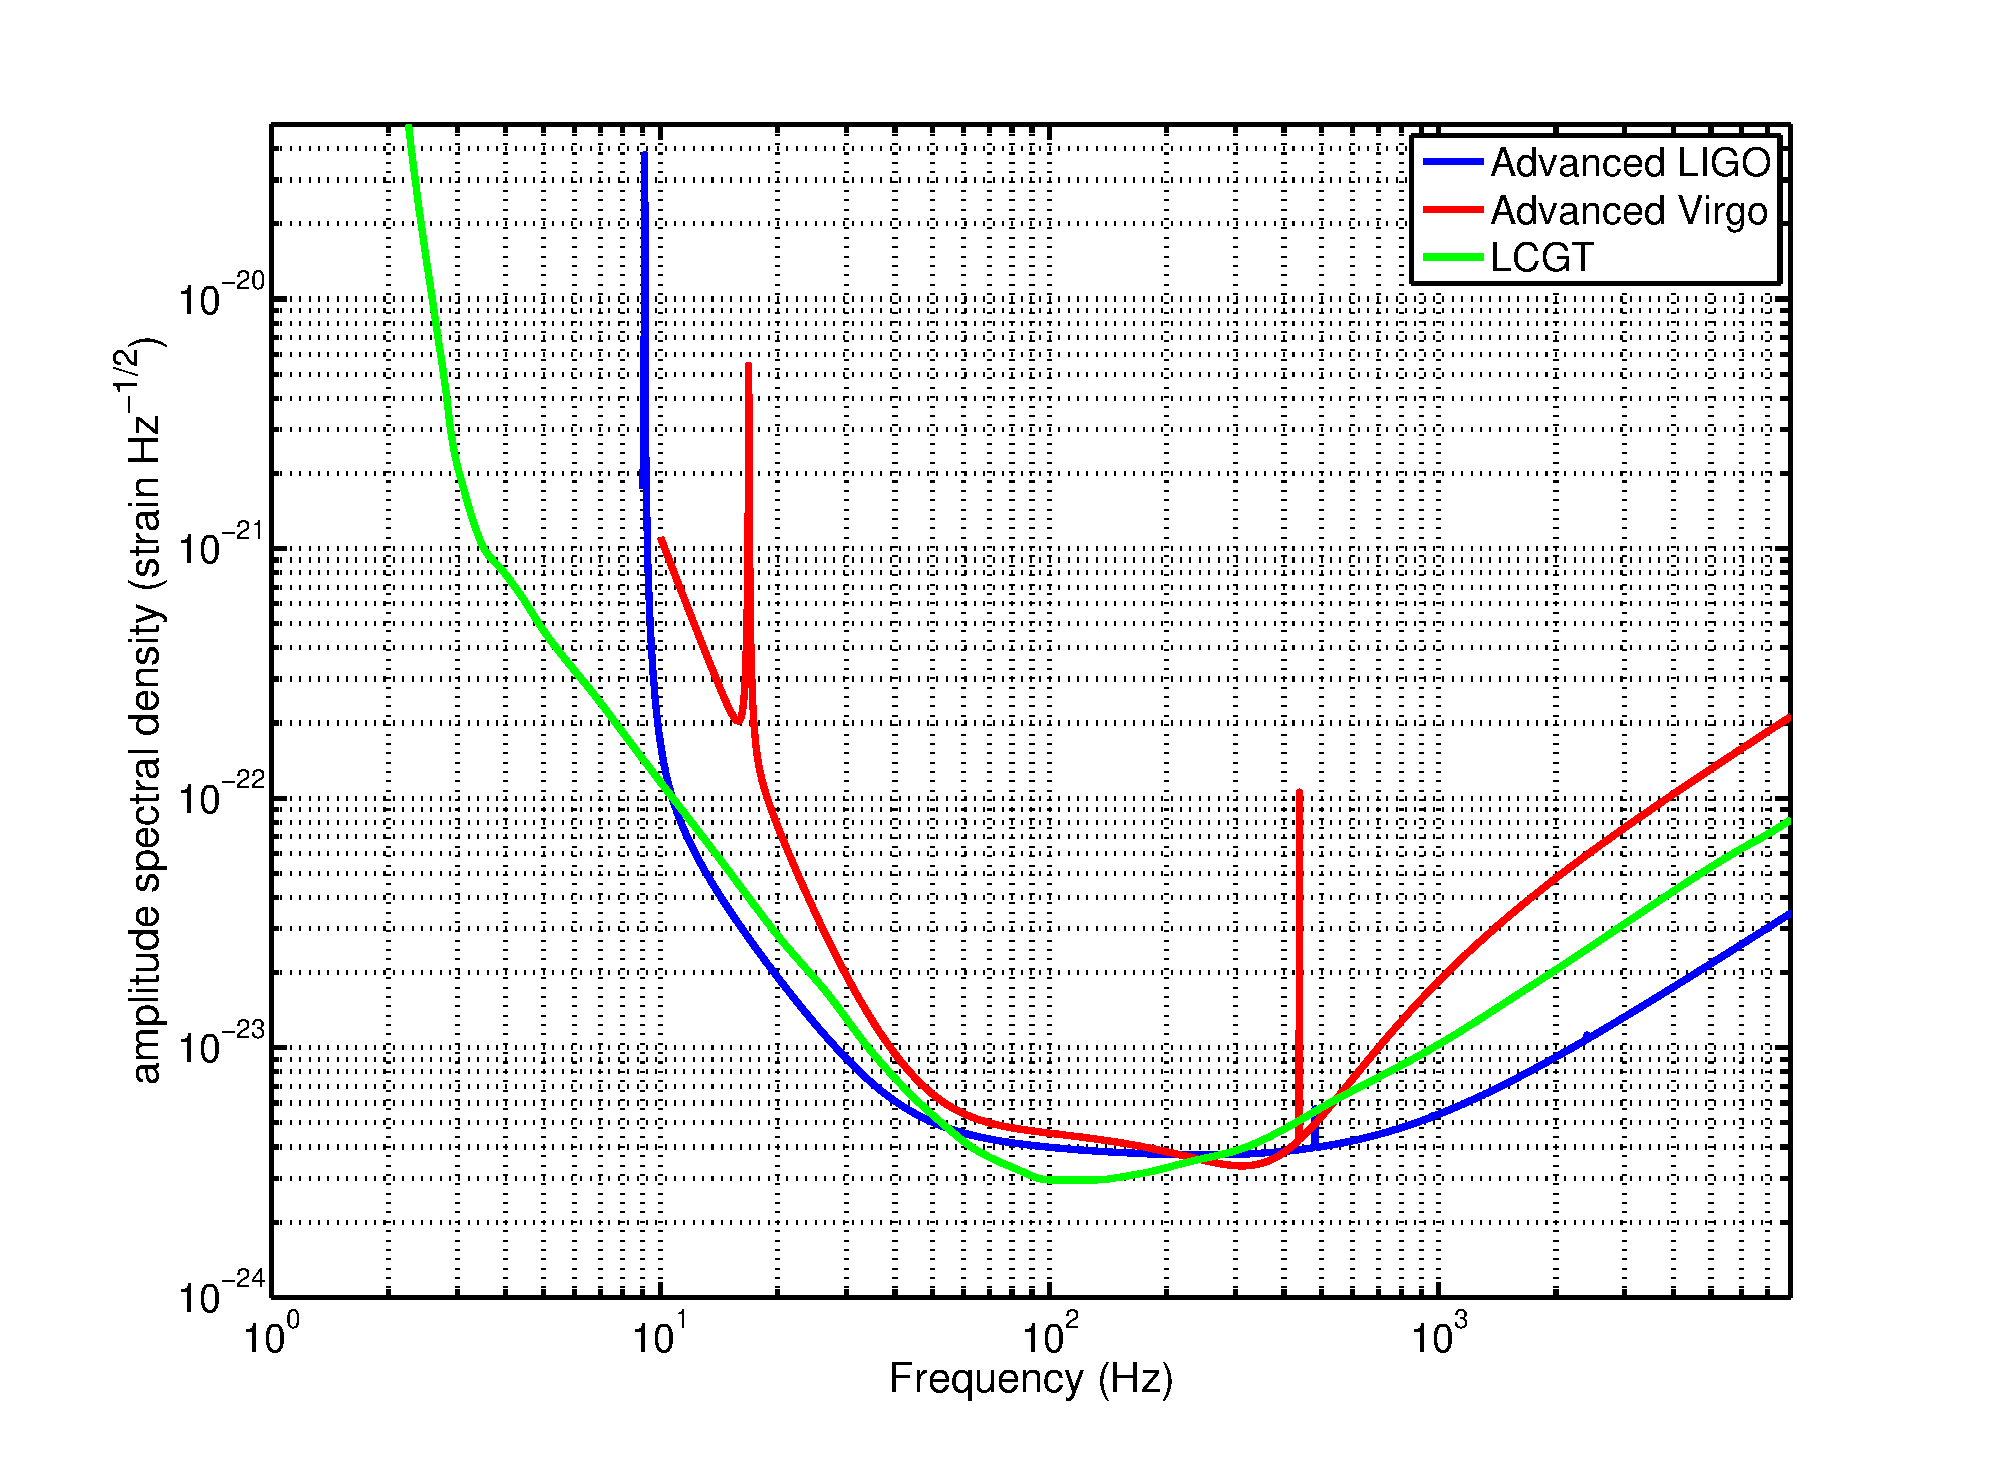
\includegraphics[scale=0.45]{advcurves}}
  \caption{\it Design sensitivity curves for the Advanced LIGO, Advanced Virgo
and LCGT second generation detectors. The Advanced LIGO curve comes from 
\cite{Harry:2010}, the Advanced Virgo curve comes from \cite{aVIRGOweb}, and the
LCGT curve comes from \cite{Arai:2009}. These curves are based on specific
configurations of the detectors and are therefore subject to change.}
  \label{fig:advcurves}
\end{figure}}

AdvVirgo will apply similar upgrades to those for aLIGO and over a similar
timescale (for details see \cite{AdVwhitepaper} and \cite{AdVdesign}). Plans are
to add a signal recycling mirror, monolithic suspensions, increased laser power
to $\sim200$~W, improved coatings a potentially use non-Gaussian beams (see 
e.g.~\cite{Freise:2010}), although this option is unlikely. The seismic isolation
system will not be changed. Virgo will shut down to begin these upgrades in July
2011.

The Large-scale Cryogenic Gravitational-Wave Telescope (LCGT)
\cite{Miyoki:2005, Ohashi:2008} is a planned Japanese detector to be sited
underground in the Kamioka mine. The LGCT will consist of two co-located
detectors with 3~km arms, using sapphire mirrors and sapphire
suspensions. Initially it will operate at room temperature, but will later be
cooled to cryogenic temperatures. This detector is planned to have similar sensitivities to aLIGO
and AdvVirgo, with a reach for binary coalescences of about 200~Mpc with SNR of
10. There currently exists a technology demonstrator called the Cryogenic Laser
Interferometer Observatory (CLIO) \cite{Yamamoto:2008, CLIOweb}, which has a
100~m baseline and is also sited in the Kamioka mine. This is to demonstrate the
very stable conditions (i.e.\ low levels of seismic noise) existing in the mine
and also the cryogenically cooled sapphire mirrors suspended from aluminium
wires. In experiments with CLIO at room temperature (i.e. 300~K), using a metallic glass 
called Bolfur for its wire suspensions, it has already been used to produce an astrophysics result by
looking for gravitational waves from the Vela pulsar \cite{Akutsu:2008}, giving
an 99.4\% confidence upper limit of $h = 5.3\times10^{-20}$. Tests with the
cryogenic system activated and using aluminium suspensions allowed two mirrors to be cooled to
$\sim14$\,K.

Having a network of comparably sensitive detectors spread widely across the globe 
is vital gain the fullest astrophysical insight into transient sources. Position
reconstruction for sources relies on triangulating the location based on time-of-flight
delays observed between detectors. Therefore have long baselines, and different planes,
between as many detectors as possible gives the best positional reconstruction -- in 
\cite{Fairhurst:2010} it is shown that for the 2 US aLIGO sites sky localisation will
be of order 1000 square degrees, whereas this can be brought down to a few square degrees
with the inclusion of more sites and detectors. 
Observation with multiple detectors also provide the best way to give confidence that a
signal is a real gravitational wave rather than the accidental coincidence of 
background noise. Finally multiple, differently oriented, detectors will increase the
ability to reconstruct a transient sources waveform and polarisation. 

\subsubsection{Third generation detectors}
Currently design studies are under way for a third generation gravitational wave
observatory called the Einstein Telescope (ET) \cite{ETweb}. This is a European
Commission funded study with working groups looking into various aspects of the
design including: the site location and characteristics (e.g. underground),
suspensions technologies; detector topology and geometry (e.g. a equilateral
triangle configuration); and astrophysical aims. This preliminary plan is to
aim for an observatory which improves upon the second generation detectors by
an order of magnitude over a broad band. There are many technological
challenges to be faced in attempting to make this a reality and research is
currently under way into a variety of these issues.

Investigations into the interferometric configuration have already been studied
(see \cite{Freise:2008, Hild:2008b, Hild:2010}), with suggestions including a triple
interferometer system made up from an equilateral triangle, an underground
location, and potentially a xylophone configuration (two independent detectors
covering different frequency ranges i.e. ultimately giving six detectors in 
total, although constructed over a period of years). Three potential sensitivity
curves are plotted in Fig~\ref{fig:etsens} for different configurations of detectors.

\epubtkImage{}{%
\begin{figure}[hptb]
  \centerline{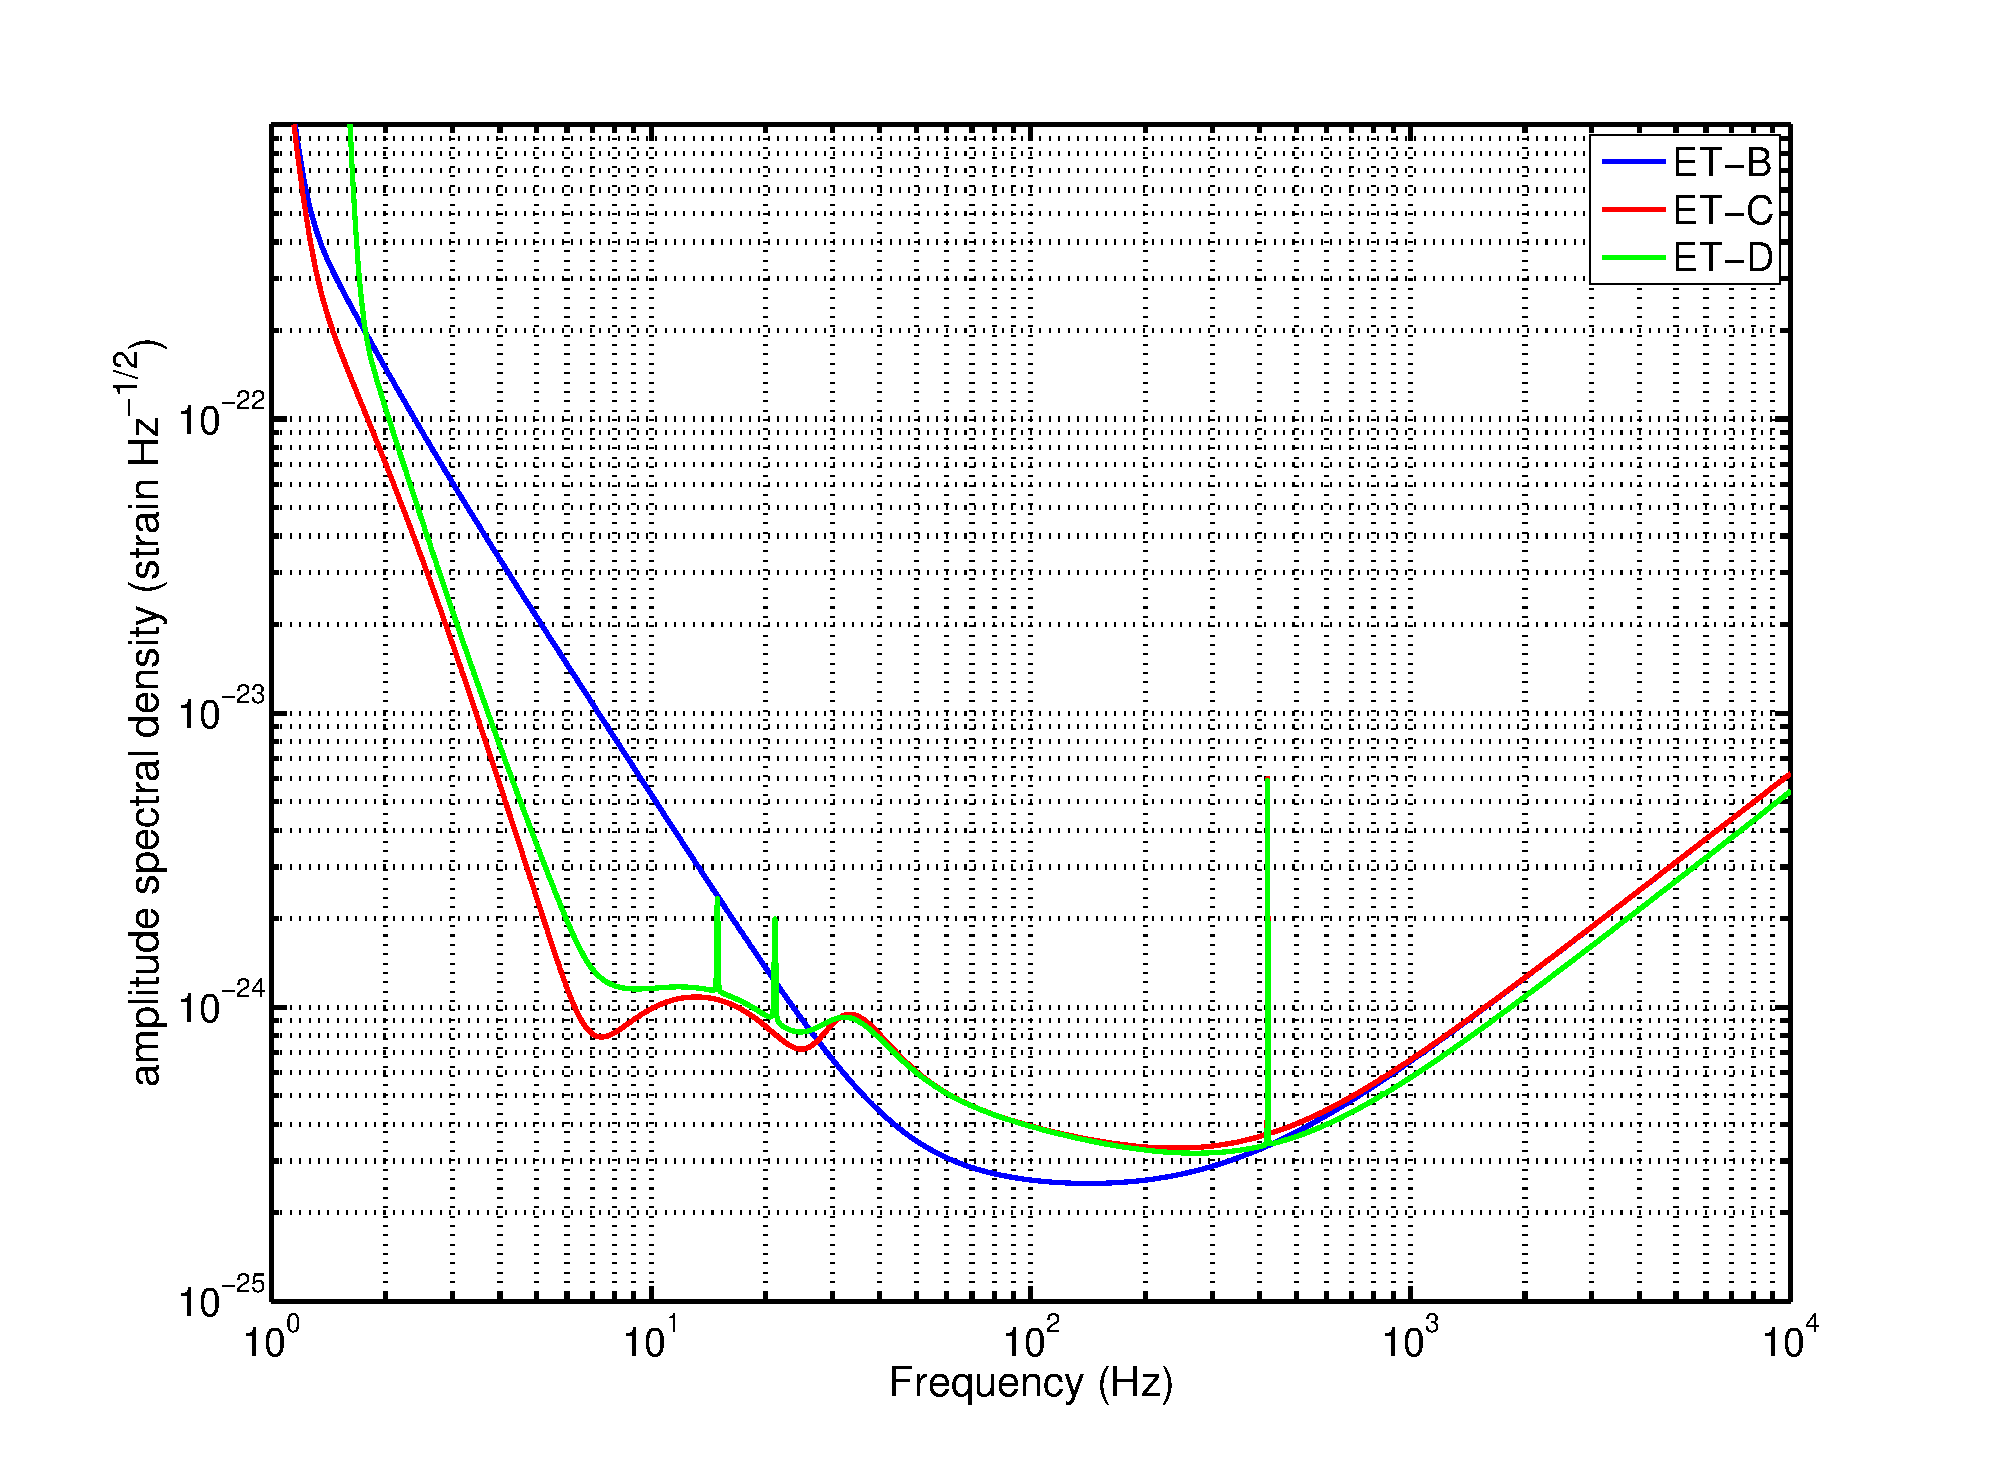
\includegraphics[scale=0.45]{etcurve}}
  \caption{\it Potential sensitivities of the Einstein Telescope for 3 different
design concepts: ET-B \cite{Hild:2008b}, ET-C \cite{Hild:2010b} and ET-D 
\cite{Hild:2010}. The curves are available from \cite{etcurves}}
  \label{fig:etsens}
\end{figure}}

%This level of sensitivity is expected to be improved on when the longer LIGO
%and Virgo detectors are upgraded. Indeed plans for an upgraded LIGO, LIGO~2,
%are already on the drawing board. Plans are to use 30~kg sapphire test masses
%for this detector, suspended by fused silica fibers or ribbons, along with an
%improved seismic isolation system, increased laser power, of the order of
%100~W, and signal recycling~\cite{Whitepaper}. The contribution of the
%different noise source to the expected interferometer sensitivity as
%contained in~\cite{Whitepaper}, is shown in
%Fig.~\ref{figure:noisecontributions}.

%\epubtkImage{}{%
%\begin{figure}[hptb]
%  \centerline{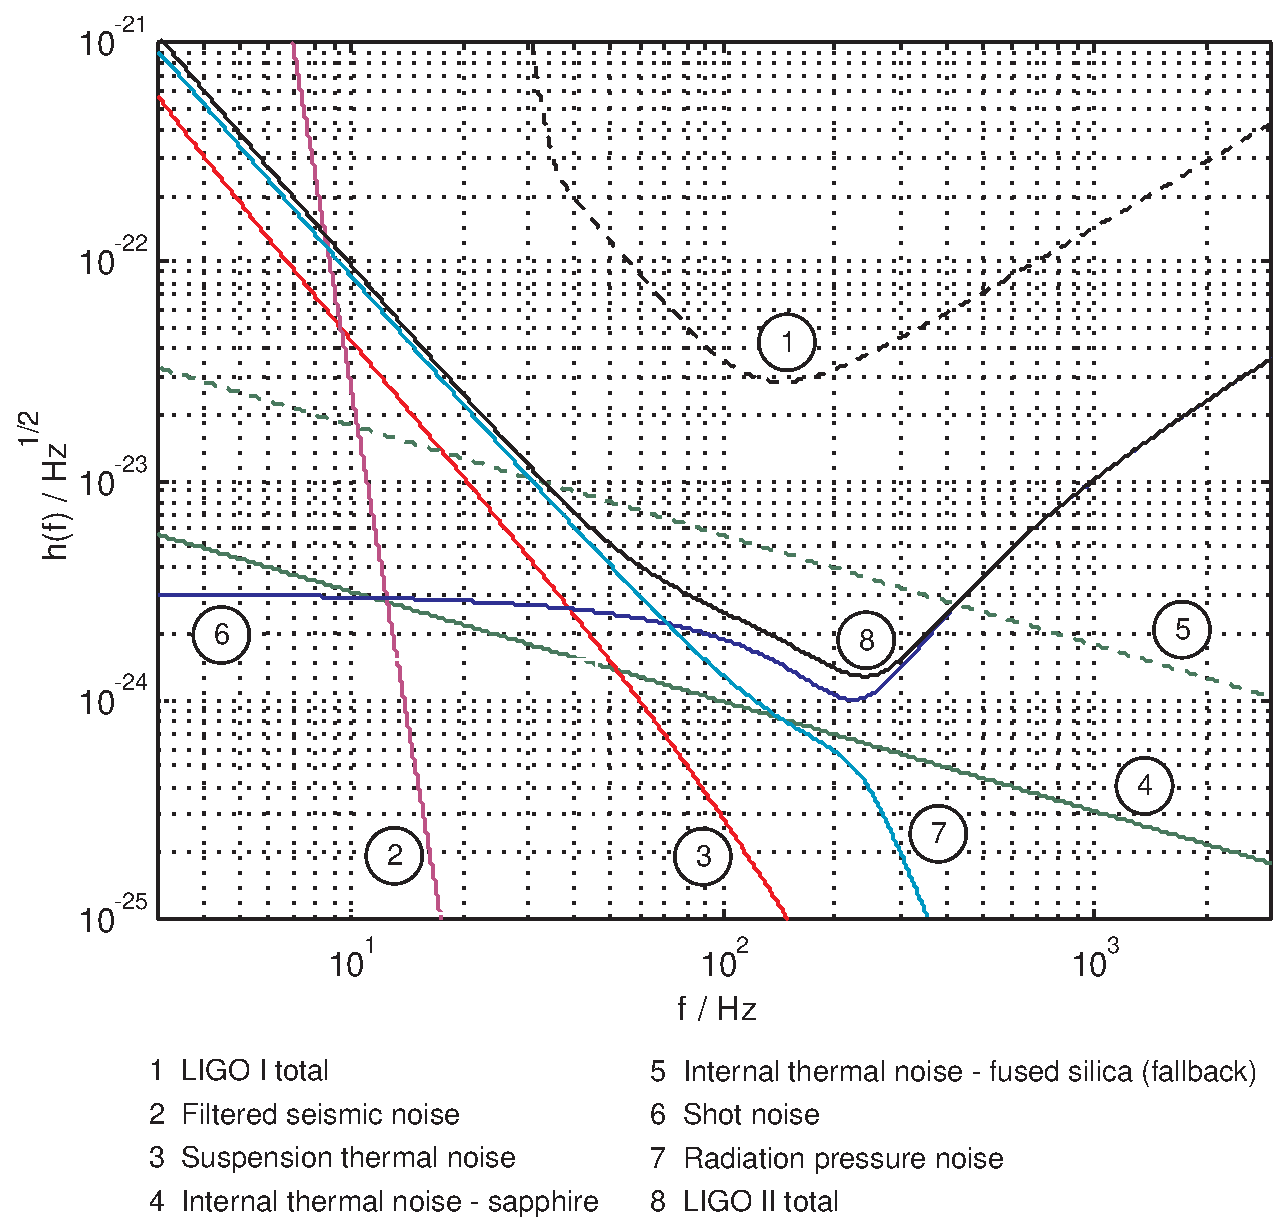
\includegraphics[scale=0.5]{noisecon}}
%  \caption{\it Noise contributions to the expected sensitivity of the
%    LIGO~2 interferometer.}
%  \label{figure:noisecontributions}
%\end{figure}}

%It should be noted that very recent work by Braginsky and colleagues
%in Moscow~\cite{Bragthermo} is suggesting that a form of mechanical
%loss known as thermoelastic damping~\cite{Nowick} is important in bulk
%crystalline materials such as as sapphire, and may be represented by a
%noise line somewhat higher than the thermal noise in the above
%figure. This is currently under investigation (at the beginning of
%2000).

%%%%%%%%%%%%%%%%%%%%%%%%%%%%%%%%%%%%%%%%%%%%%%%%%%%%%%%%%%%%%%%%%%%%%%%%%%%%%%%%
%%%
%%%%%%%%%%%%%%%%%%%%%%%%%%%%%%%%%%%%%%%%%%%%%%%%%%%%%%%%%%%%%%%%%%%%%%%%%%%%%%%%
%%%
%%%%%%%%%%%%%%%%%%%%%%%%%%%%%%%%%%%%%%%%%%%%%%%%%%%%%%%%%%%%%%%%%%%%%%%%%%%%%%%%
%%%

\newpage

\section{Longer Baseline Detectors in Space}
\label{section:space}

Some of the most interesting gravitational wave signals, resulting from the
mergers of supermassive black holes in the range $10^3$ to $10^6$\,M$_{\odot}$
and cosmological stochastic backgrounds, will lie in the frequency region below
that of ground-based detectors. The most promising way of looking for such
signals is to fly a laser interferometer in space, i.e.\ to launch a number of
drag free spacecraft into orbit and to compare the distances between test
masses in these craft using laser interferometry.

\subsection{LISA}
The Laser Interferometer Space Antenna (LISA) (see for example~\cite{LISAsymposium,
NASAweb, ESAweb}) is a planned joint ESA/NASA mission to observe these low frequency
gravitational waves, with a sensitive frequency band between 0.1\,mHz and
0.1\,Hz (a reference sensitivity curve is given in Fig~\ref{fig:lisasens}). 
It will consist of an array of three drag-free spacecraft at the vertices
of an equilateral triangle of length of side $5\times10^6$~km, with the cluster 
placed in an Earth-like orbit at a distance of 1~AU from the Sun,
$20^{\circ}$ behind the Earth and inclined at $60^{\circ}$ to the ecliptic. A
current review of LISA technologies, with expanded discussion of, and references
for, topics touched upon below, can be found in \cite{Jennrich:2009}. Here we
will focus upon a couple of topics regarding the interferometry needed to give
the required sensitivity.

\epubtkImage{}{%
\begin{figure}[hptb]
  \centerline{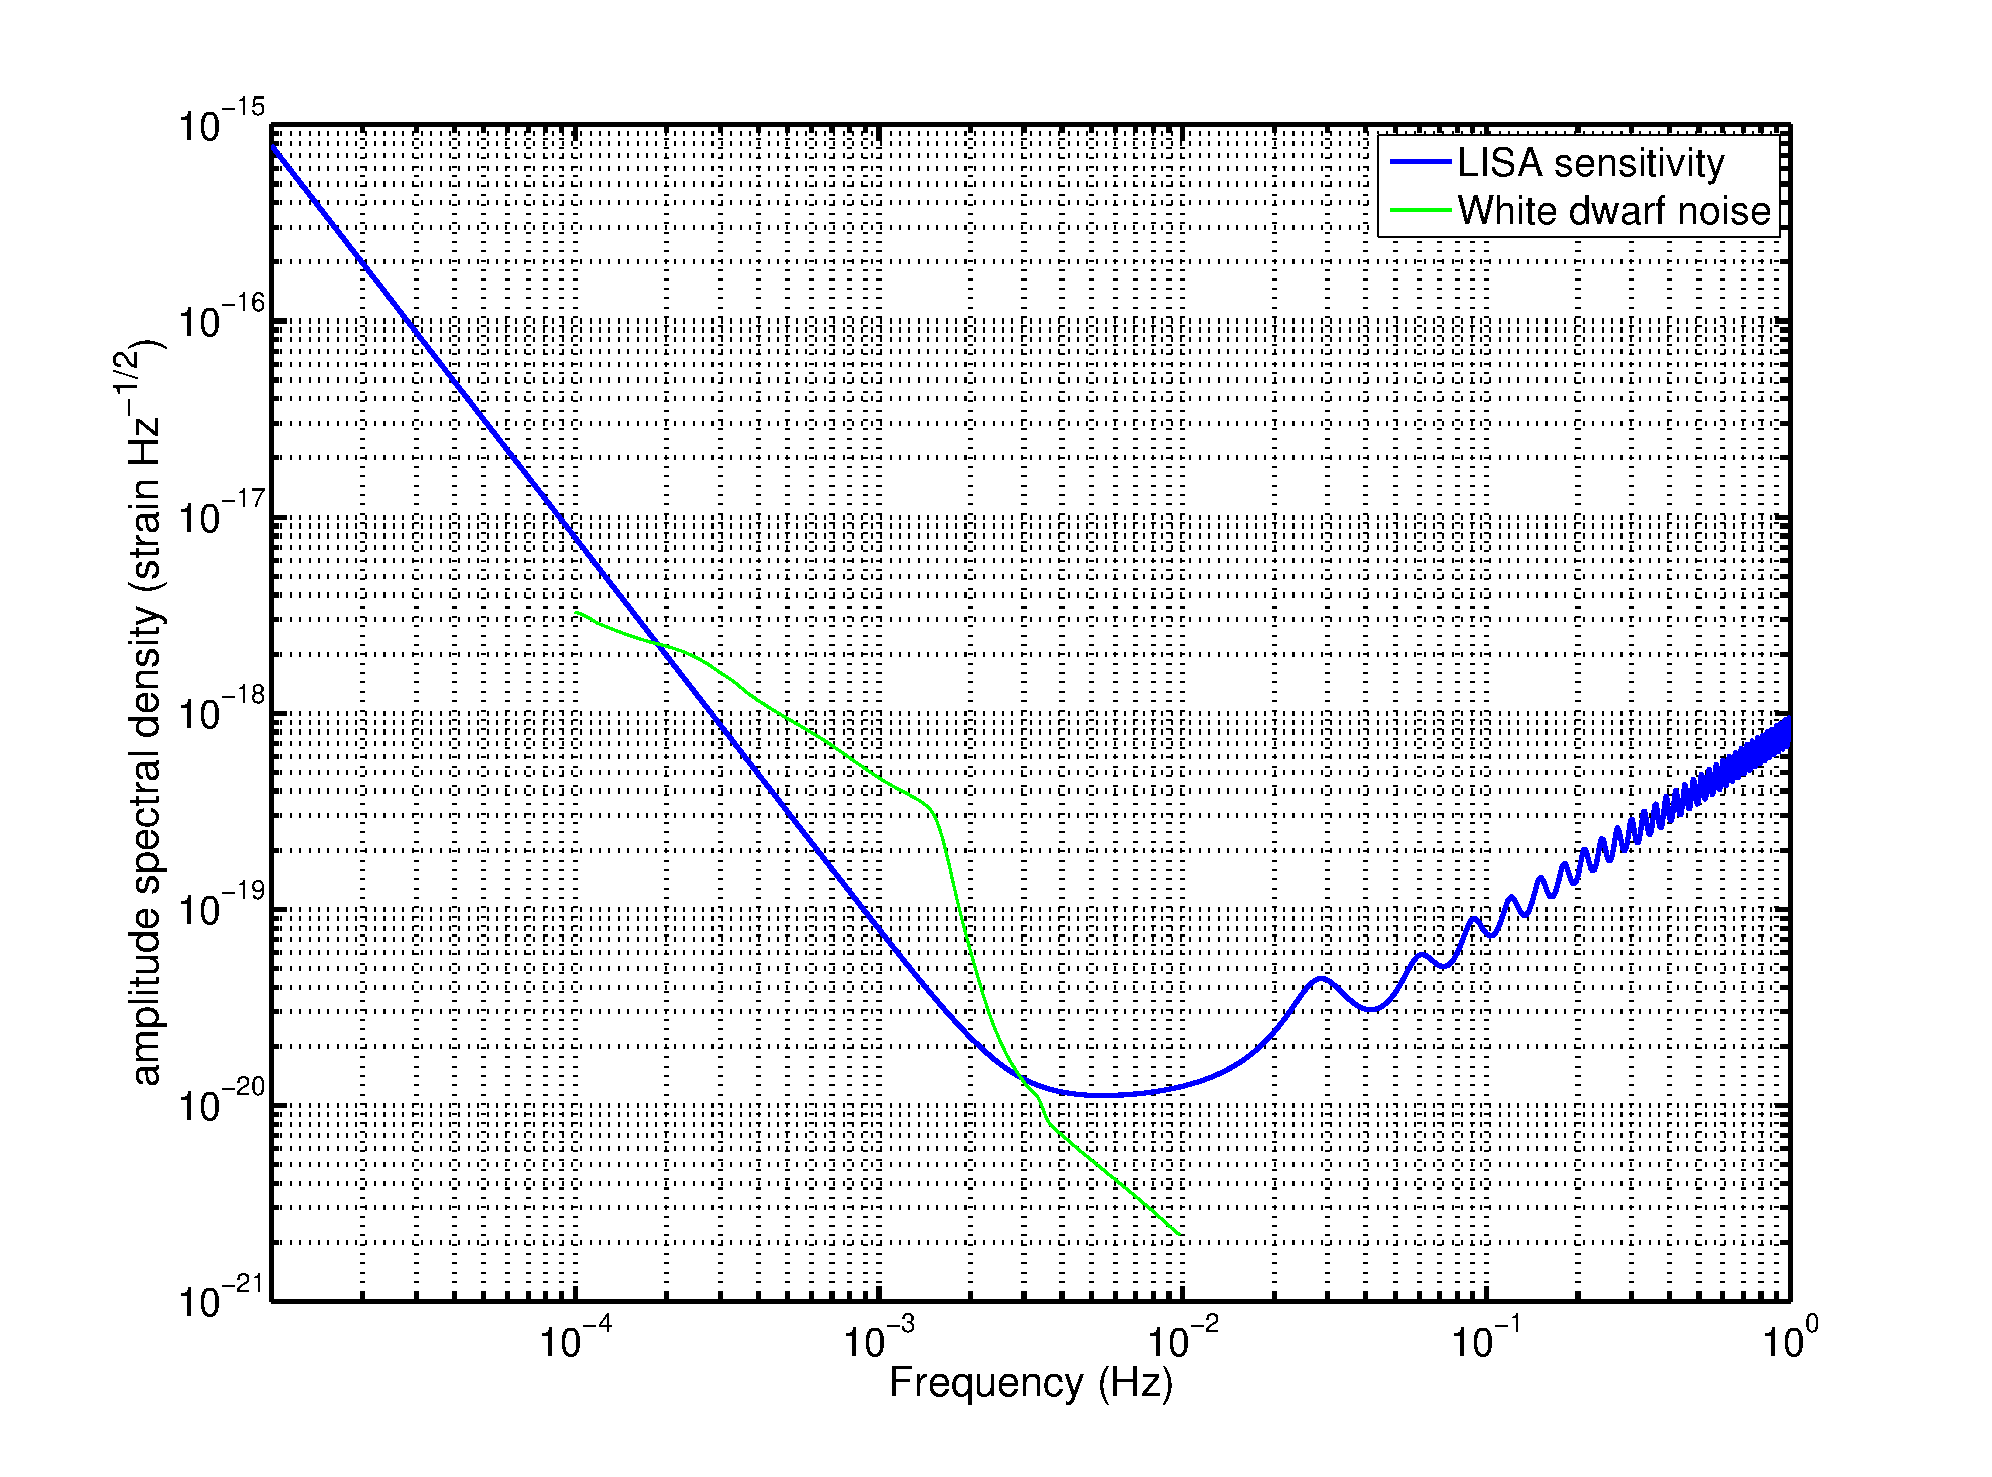
\includegraphics[scale=0.45]{lisacurve}}
  \caption{\it A design sensitivity curves for LISA created using the online
generator at \cite{lisasens}. Also included is a curve showing the expected
background noise from galactic white dwarf binary systems, which will dominate
over the instrumental noise in the range from $\approx$0.1--1~mHz.}
  \label{fig:lisasens}
\end{figure}}

Proof masses inside the spacecraft (two in each spacecraft) form the end points
of three separate, but not independent, interferometers. Each single two-arm 
Michelson type interferometer is formed from a vertex (actually consisting of
the proof masses in a `central' spacecraft), and the masses in two remote
spacecraft as indicated in Fig.~\ref{figure:LISA}. The 
three-interferometer configuration provides redundancy against component
failure, gives better detection probability, and allows the determination of the
polarisation of the incoming radiation. The spacecraft which house the optical benches
are essentially there as a way to shield each pair of proof masses from external disturbances (e.g.
solar radiation pressure). Drag free control servos enable the spacecraft to
follow the proof masses to a high level of precision, the drag compensation
being effected using proportional electric thrusters. Illumination of the
interferometers is by highly stabilised laser light from Nd:YAG lasers at a
wavelength of 1.064 microns, laser powers of $\simeq$2~W being available from
monolithic, non planar ring oscillators which are diode pumped.  For LISA
to achieve its design performance strain sensitivity of around $10^{-20}\,{\rm
Hz}^{-1/2}$, adjacent arm lengths have to be sensed to an accuracy of about $10
{\rm \ pm}(\rm Hz)^{-1/2}$. Because of the long distances involved and the
spatial extent of the laser beams (the diffraction limited laser spot size,
after travelling $5\times10^{6}$~km, is approximately 50~km in diameter), the
low photon fluxes make it impossible to use standard mirrors for reflection;
thus active mirrors with phase locked laser transponders on the spacecraft will
be implemented. Telescope mirrors will be used to reduce diffraction losses on
transmission of the beam and to increase the collecting area for reception of
the beam. With the given laser power, and using arguments similar to those already 
discussed for ground based detectors with regard to photoelectron shot noise 
considerations, means that for the required sensitivity the transmitting and 
receiving telescope mirrors on the spacecraft will have diameters of 40~cm.

\epubtkImage{}{%
\begin{figure}[hptb]
  \centerline{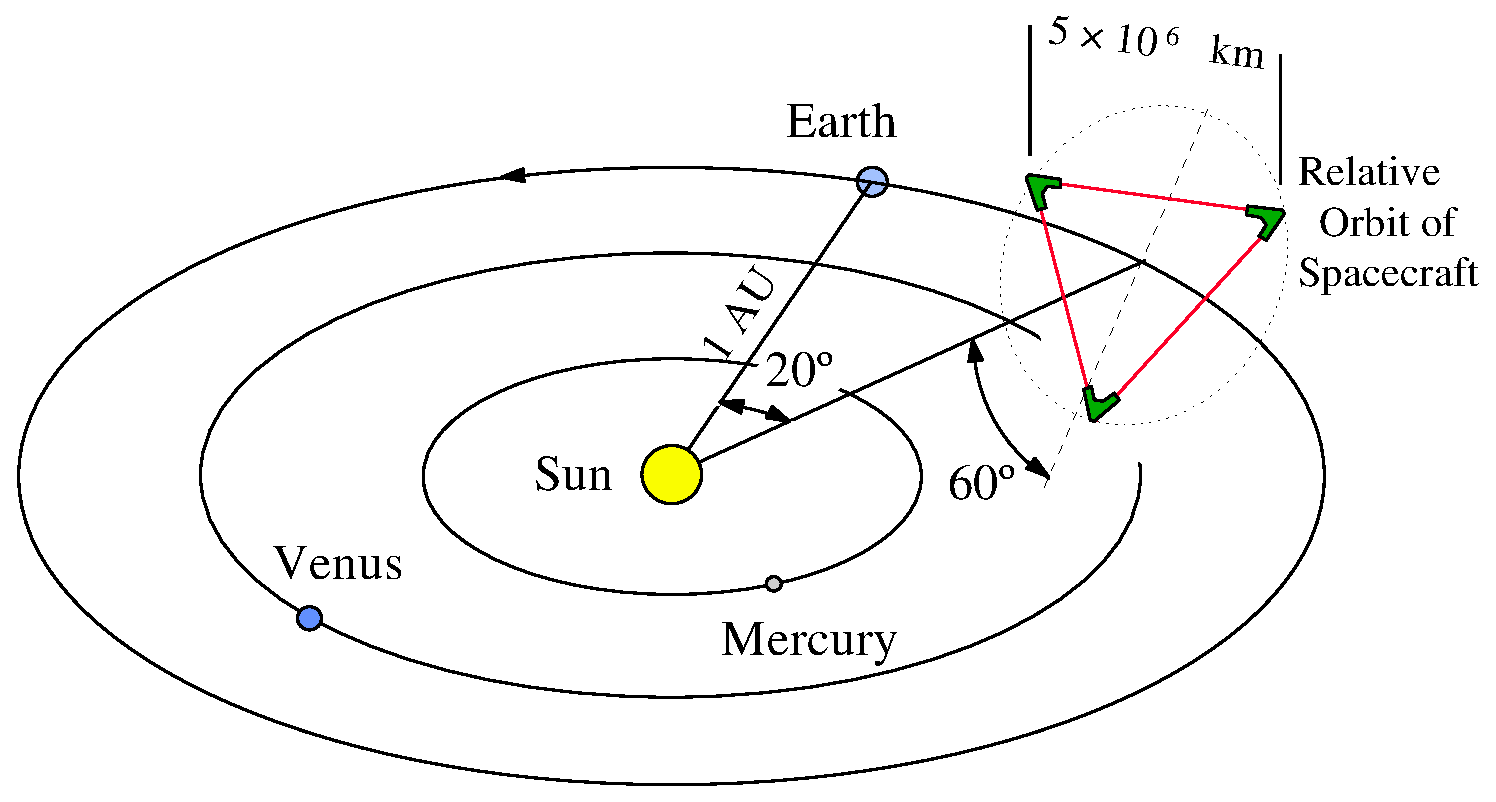
\includegraphics[scale=0.4]{fig8}}
  \caption{\it The proposed LISA detector.}
  \label{figure:LISA}
\end{figure}}

Further, just as in the case of the ground based detectors, the presence of
laser frequency noise is a limiting factor. It leads to an error in the
measurement of each arm length. If the arms are equal these errors cancel out,
but if they are unequal the comparison of lengths used to search for
gravitational waves may be dominated by frequency noise. For the
$5\times10^9$~m long arms of LISA, a difference in arm length of $10^8$~m is 
likely. Then for a relative arm length measurement of $2 \times 10^{-12}\,{\rm
m}\,{\rm Hz}^{-1/2}$ (the error budget level allowed in the LISA design for this
noise source), Equation~(\ref{equation:frequnoise}) suggests that a laser
stability of $\simeq 6 \times 10^{-6}\,{\rm Hz}\,{\rm Hz}^{-1/2}$ is required, a
level much better than can be achieved from the laser on its own. Thus frequency
stabilisation has to be provided. The first method of stabilisation is to lock
the frequency of one laser in the system on to a local frequency reference, 
e.g.\ a Fabry-Perot cavity mounted on one of the craft (see for
example~\cite{McNamara}), and then to effectively transfer this stability to
other lasers in the system by phase locking techniques. With the temperature
fluctuations inside each craft limited in the region of 3~mHz to
approximately $10^{-6}\,{\rm K}\,{\rm Hz}^{-1/2}$ by three stages of thermal
insulation, a cavity formed of material of low expansion coefficient such as ULE
allows a stability level of approximately $30 {\rm Hz}{\rm Hz}^{-1/2}$ (again
at 3~mHz). This level of laser frequency noise is clearly much worse than the
required $1.2 \times 10^{-6}\,{\rm Hz}\,{\rm Hz}^{-1/2}$ (at 3\,mHz) and a
further correction scheme is needed. A second possible stage of frequency
stabilisation is arm-locking \cite{Sheard:2003}, which relies on the fact that
by design the fractional stability of the LISA arms is of order $\delta{}l/L
\sim 10^{-21}\,{\rm Hz}^{-1/2}$ to derive an error signal from the phase 
difference between the local laser and the received light. As the received light
is phase locked with the local laser from the craft that sent it it caries a
replica of the frequency noise of the local laser noise delayed by one round
trip time $\tau=33$\,s. Using this fact this noise can be suppressed at frequencies smaller
than the round trip frequency $f= 1/\tau = 30$\,mHz. This scheme requires no
additional hardware and can be completely implemented in software, but it will
still leave frequency noise that is several orders of magnitude above required
levels. A third stage frequency stabilisation scheme, which is a post-processing
step, is time-delay interferometry (TDI). This makes use of the fact that,
because the beams coming down each arm are not combined, the phase of each beam can
be measured and recorded. Therefore correlations in the frequency noise can be
calculated and subtracted by algebraically combining phase measurements from
different craft delayed by the multiples of the time delay between the spacecraft.
The accuracy of this is set by the phase measurement accuracy, which allows
frequency noise subtraction to below the required level. A simple TDI scheme,
for a much simplified constellation, was first based in the frequency domain
\cite{Giampieri}, but due to complexities in taking into account changing arm
lengths and a more complex interferometric scheme subsequent implementations have
been in the time domain. A mathematical overview of the TDI scheme, along with
moving spacecraft and unequal arm lengths, can be found in \cite{Tinto:2005}.

One of the major components of LISA is the disturbance reduction system (DRS),
which is responsible for making sure the test masses follow, as far as
possible, purely gravitational orbits. This consists of the gravitational
reference sensor (GRS) and the control and propulsion systems used to keep the
spacecraft centred on the test mass. The test masses for LISA are 1.96\,kg
cubes, with sides of 46\,mm and made of an alloy of 75\% gold and 25\% platinum,
chosen because of its very small magnetic susceptibility. The masses are housed
in a cube of electrodes designed to capacitively sense their position and
to have measurement noise levels of 1.8\,nm\,Hz$^{-1/2}$. The masses need to be
tightly held in place during launch and then released, so a caging mechanism
has been designed consisting of 8 hydraulic fingers (one for each corner of the
mass) pushing with 1200\,N of force. There will be adhesion between the fingers
and the masses, which will require about 10\,N of force per finger to break. To
provide this force two plungers will push on the the top and bottom surfaces of
the masses releasing them from the fingers, followed by pushing smaller release
tips in each plunger, and quickly retracting them, to overcome their adhesion to
the masses. Charged particles produced by cosmic radiation interacting with the
surrounding spacecraft can cause the test masses to become charged at a rate of
about 50 electrons per second. Current plans are to use UV light from mercury
lamps (or potentially UV LEDs) to discharge the masses. Another key technology
for the DRS are the micro-Newton thrusters, which provide the fine control
needed for drag-free flight. These will mainly be used to counteract solar
radiation pressure on the spacecraft, which requires about 10\,$\mu$N per
relevant thruster. Thrust noise as a function of frequency is required to be
smaller than $0.1\,\mu{\rm N}\,{\rm
Hz}^{-1/2}\times\sqrt{1+\left(\frac{10\,{\rm m}\,{\rm Hz}}{f}\right)^4}$. Two
types of system, both of which meet the requirements, will be tested on LISA
Pathfinder: the US colloid micro-Newton thruster (CMNT); and the European field
emission electric propulsion system (FEEP). The CMNT uses small drops of a
colloid, which it ionises through field emission, accelerates and ejects from
the thruster. Two designs of FEEP currently exist, one using indium and the
other caesium and with different geometries, which instead of ionising a droplet
of colloid just use single ions. This means FEEPs have a better charge to mass
ratio. The current baseline is to use caesium FEEPs. Many of these systems above
are being tested in the LISA Pathfinder mission (see below) and use the nominal
LISA designs.

There are many other issues associated with the laser interferometry, and other
aspects of the mission mentioned above, for LISA which are not dealt with here
and the interested reader should refer to~\cite{Houghetal, Jennrich:2009,
Johann:2008} for a discussion of some of these.

For LISA the baseline mission design was finalised in 2005. An industrial
contract was awarded to Astrium GmbH for the LISA Mission Formulation study
\cite{Johann:2008}. Within the current ESA Science Programme LISA is in the
Cosmic Vision 2015-2025 Programme, and launch after 2020 seems likely. 
In 2007 the National Research
Council report on the NASA Beyond Einstein Program (soon to become the Physics
of the Cosmos Program) gave LISA the highest scientific ranking, and it has
been rated very highly in the Astro2010 decadal survey \cite{astro2010}. Recent
technical reports for LISA can be found at \cite{LISATechReports}.

Several of the key technologies for LISA are being testing on the LISA
Pathfinder mission (formerly SMART-2). Details of the current status of this
mission can be found in \cite{Armano:2009}. LISA Pathfinder, will fly the
LISA Technology Package (LTP), which essentially consists of a downscaled
version of one LISA arm compressed from 5 million km to 38\,cm. The LTP {\it arm}
contain two test masses (an emitter and a receiver) with a Doppler link
between them. The three main things it will measure are: the acceleration phase
noise caused by the relative motion of the emitter and receiver from
non-gravitational forces; the readout noise; and noise caused by the departure
of the Doppler link from the ideal scheme, due to the fact that we are not
truly measuring the relative accelerations of two point particles, but instead
a more complex systems of multiple Doppler links and extended masses. It is
designed to test the accuracy of these to within an order of magnitude of that required by
the full LISA. Other aspects of the mission that will be tested are the
discharging of the test masses, the caging and release of the masses following
launch and the $\mu$Newton thrusters. As much as possible the nominal LISA
systems and hardware are being used. LISA Pathfinder is currently scheduled for
launch in mid 2013, after which it will orbit the L1 point, with a 180 day
mission plan.

\subsection{Other missions}
LISA is the most advanced space-based project, but there exist concepts for at
least two more detectors. DECIGO (DECi-hertz Interferometer Gravitational Wave
Observatory) \cite{Sato:2009} is a Japanese project designed to fill the gap in
frequency between ground-based detectors and LISA, i.e.\ the 0.1--10\,Hz band. It
would have a similar configuration to LISA with three drag-free spacecraft, but
have far shorter arm lengths at 1000\,km. Although still early in its design
there are plans for two precursor technology demonstration missions (DECIGO
Pathfinder \cite{Ando:2009} and Pre-DECIGO), with a the main mission having a
launch date in the mid-2020s.

A similar mission, in terms of the frequency band it seeks to cover, is the US
Big Bang Observer (BBO) (see \cite{Crowder:2005, Cutler:2009, Harry:2006} for
overviews of the proposal). One of its main aims will be to detect the
stochastic background from the early universe, but it can also be used for high
precision cosmology \cite{Cutler:2009}. The current configuration would consist
of three LISA-like constellations of three spacecraft each, with 50\,000\,km arm
lengths, and separated in their orbit by $120^{\circ}$. The launch of this
mission would be after DECIGO, but is designed to be 2--3 times as sensitive.

At lower frequencies than LISA, $\sim0.1\,\mu{\rm Hz}$--$1\,{\rm mHz}$, there
are Chinese proposals for Super-ASTROD (Super Astrodynamical Space Test of
Relativity using Optical Devices) \cite{Ni:2009}.

%%%%%%%%%%%%%%%%%%%%%%%%%%%%%%%%%%%%%%%%%%%%%%%%%%%%%%%%%%%%%%%%%%%%%%%%%%%%%%%%
%%%
%%%%%%%%%%%%%%%%%%%%%%%%%%%%%%%%%%%%%%%%%%%%%%%%%%%%%%%%%%%%%%%%%%%%%%%%%%%%%%%%
%%%
%%%%%%%%%%%%%%%%%%%%%%%%%%%%%%%%%%%%%%%%%%%%%%%%%%%%%%%%%%%%%%%%%%%%%%%%%%%%%%%%
%%%

\newpage

\section{Conclusion}
\label{section:conclusion}

Significant effort worldwide has been invested, and is continuing to be invested, in the development
of both ground and spaced based gravitational wave detectors. Over the coming years, ground-based
detectors will reach sensitivities that will enable the direct observation of gravitational waves as predicted by Einstein's
General Theory of Relativity and open the exciting new field of gravitational wave astronomy. Studying the gravitational wave
sky could radically change our understanding of the Universe, expanding our knowledge of fundamental physics, cosmology and
relativitic astrophysics. Gravitational wave observations will allow us to gaze into the heart of the most violent events in the
Universe, and will help answer some of the biggest questions, particularly is cosmology when combined with other astronomical observations.



%%%%%%%%%%%%%%%%%%%%%%%%%%%%%%%%%%%%%%%%%%%%%%%%%%%%%%%%%%%%%%%%%%%%%%%%%%%%%%%%
%%%
%%%%%%%%%%%%%%%%%%%%%%%%%%%%%%%%%%%%%%%%%%%%%%%%%%%%%%%%%%%%%%%%%%%%%%%%%%%%%%%%
%%%
%%%%%%%%%%%%%%%%%%%%%%%%%%%%%%%%%%%%%%%%%%%%%%%%%%%%%%%%%%%%%%%%%%%%%%%%%%%%%%%%
%%%

\newpage

\section{Acknowledgements}
\label{section:acknowledgements}

We would like to thank our colleagues in the GEO~600 project and at Stanford
University for useful discussions. We are grateful to the LSC and the Virgo
groups for the use of some of their figures. We are indebted to STFC (U.K.), NSF
(U.S.A.), the University of Glasgow and Stanford University, and the Royal Society of Edinburgh for support.



%%%%%%%%%%%%%%%%%%%%%%%%%%%%%%%%%%%%%%%%%%%%%%%%%%%%%%%%%%%%%%%%%%%%%%%%%%%%%%%%%%%
%%%%%%%%%%%%%%%%%%%%%%%%%%%%%%%%%%%%%%%%%%%%%%%%%%%%%%%%%%%%%%%%%%%%%%%%%%%%%%%%%%%
%%%%%%%%%%%%%%%%%%%%%%%%%%%%%%%%%%%%%%%%%%%%%%%%%%%%%%%%%%%%%%%%%%%%%%%%%%%%%%%%%%%

\newpage

\bibliography{refs}



\end{document}

